\documentclass[engineer,fontset=windows,nocolorlinks]{seumasterthesis}
\raggedbottom
% \makeatletter    盲审稿设置
% \renewcommand{\cleardoublepage}{%
%   \clearpage
%   \if@twoside
%     \ifodd\c@page
%     \else
%       \stepcounter{page}%
%     \fi
%   \fi
% }
% \makeatother
\begin{document}

%% ----------------------------------------------------------------------------
%%                                 Meta Data
%% ----------------------------------------------------------------------------
\categorynumber{TP242.6}         % Chinese Library Classification
\UDC{007.52}                    % Universal Decimal Classification
\secretlevel{公开}                % Secret Level
\studentid{233667}              % Student Number

%% ----------------------------------------------------------------------------
%%                           Thesis Title and Spine
%% ----------------------------------------------------------------------------
\title
    {基于特征时序缓存视觉语言动作模型的机械臂自主操作技术}                                      % Thesis Title
    {}                                          % Thesis Subtitle
    {Robot Manipulation Technology Based on Vision-Language-Action Models with Temporal Feature Cache}  % Thesis English Title
    {}            % Thesis English Subtitle

\spine
    {基于特征时序缓存视觉语言动作模型的机械臂自主操作技术}      % Spine Title
    {}                                                          % Spine Subtitle

%% ----------------------------------------------------------------------------
%%                             Author and Advidor
%% ----------------------------------------------------------------------------
\author
    {{\bfseries 刘立奥}}
    {{\bfseries Liu Liao}}

\advisor
    {{\bfseries 秦文虎~~教授 }}
    {{\bfseries Qin Wenhhu }}
    {Prof.}


%% ----------------------------------------------------------------------------
%%                              Thesis Defence
%% ----------------------------------------------------------------------------
\engthesistype{应用研究}            % Engineering Master Thesis Type
\degreetype                     % Degree Type
    {电子信息}
    {Master of Engineering}
\majors{电子信息}
\major{仪器仪表工程}                  % First-level Discipline Name
\submajor{智能机器人}               % Second-level Discipline Name
\defenddate{2026年5月29日}         % Defence Date
\authorizedate{}      % Degree Award Date
\committeechair{周军~~研究员}             % Chairman of Defence Committee
\reviewer{YS022260199}{YS022260200}             % Thesis Reviewer(s)
\department                     % Faculty or Department
    {仪器科学与工程学院}
    {School of Instrument Science and Engineering}
% \seuthesisthanks                % Short Acknowledgement
%     {本文的部分工作受--基金 No. -- 的支持与帮助，在此表示感谢。}

%% ----------------------------------------------------------------------------
%%                                  Cover
%% ----------------------------------------------------------------------------
\makebigcover
\makecover
	
%% ----------------------------------------------------------------------------
%%                          Abstract and Contents
%% ----------------------------------------------------------------------------
%% ----------------------------------------------------------------------------
%%                              Chinese Abstract
%% ----------------------------------------------------------------------------
\begin{abstract}{机械臂操作, 模仿学习, 扩散模型, 视觉语言动作模型, 时序缓存}
随着人工智能与机器人技术的不断发展，具身智能作为连接数字世界与物理世界的桥梁，正成为科技发展的重点领域。然而，真实世界中的非结构化环境往往伴随着光照变化、物体层叠遮挡等复杂因素，且长视野任务中存在时序特征上下文依赖，导致机械臂在复杂操作任务中的成功率与可靠性受到严重影响。因此，本文针对长时序、非结构化任务中的多模态动作生成与决策依赖难题，提出了一种基于特征时序缓存的视觉语言动作模型TemporalCacheVLA，为实现通用机器人控制提供了有效途径。本文的主要研究工作如下：

针对机械臂在笛卡尔空间与关节空间之间的运动映射问题，研究了基于运动学理论与典型模仿学习算法的机器人操作基础理论。该方法采用Denavit-Hartenberg参数法对Franka Panda与UR5e两款机械臂进行运动学建模，推导了正向与逆向运动学方程。为了建立机器人各关节角度与末端空间位姿的精确映射关系，明确了各参数的几何意义与计算过程。基于自建数据集完成了对真实场景动作标签的计算，为后续算法的设计与实现提供了正运动学支撑。

针对传统行为克隆方法难以有效拟合多模态动作分布的问题，提出了一种基于扩散模型的模仿学习动作生成算法。该方法采用迭代DiT作为核心去噪网络，利用EfficientViT提取轻量化多尺度视觉特征。为了实现多模态特征的有效融合，设计了非对称跨模态注意力机制，在保留状态残差的同时引导多步去噪过程，并采用DDIM策略加速采样。在RoboMimic数据集上完成了对该模型的效果评估，实验结果表明，相比于Diffusion Policy基线模型，本文方法在Transport ph任务上将成功率提升至$0.862$，在Tool Hang ph任务上达到$0.791$，同时在Transport mh任务上的成功率由$0.643$提高至$0.801$，有效平衡了复杂动作生成的质量与推理效率。

针对机器人在长时序任务中因单帧决策导致的状态混淆与上下文遗忘问题，提出了一种基于特征时序缓存的视觉语言动作模型TemporalCacheVLA。该方法采用DINOv2与SigLIP双分支视觉编码器提取特征，并结合LLaMA 2提取语义向量，同时通过SE模块压缩感知向量。为了高效维护时序上下文，设计了双通道特征时序缓存机制，通过交叉注意力检索模块与可学习门控融合模块在决策时动态融合历史上下文，并引入基于余弦相似度的缓存压缩策略。基于LIBERO基准数据集完成了对该模型的效果评估，实验结果表明，本文方法在强调指令跟随的Goal子集与包含长时序任务的LIBERO-100子集上分别取得了$95.9$和$94.9$的平均成功率。同时，在LIBERO-100子集上的消融实验表明，移除缓存检索、门控融合与缓存压缩机制分别导致成功率下降至$86.2$、$83.5$和$82.3$，验证了该缓存机制在缓解长视距任务决策波动问题上的有效性。

针对视觉语言动作模型向真实物理世界迁移部署时面临的数据采集与系统集成难题，搭建了基于GELLO遥操臂的真实物理平台并完成了系统部署与有效性验证。该方法利用与UR5e运动学等价的缩比遥操臂采集包含纠错轨迹的示教数据，对模型进行参数冻结微调。为了实现从高层语义到低层电机的安全控制，基于ROS框架开发了包含会话校验与动作限幅的本地控制节点，并将其部署为Flask远端推理服务。在真实UR5e机械臂平台上完成了对模型的实机效果评估，实验结果表明，TemporalCacheVLA在简单抓取、抽屉操作及长时效组合任务中分别取得了$85$、$65$和$40$的成功率。相比于OpenVLA基线模型，本文方法在长时效组合任务中的成功率提升了$30$个百分点，证明了所提框架在真实物理环境中的可行性与实际应用价值。

\end{abstract}

%% ----------------------------------------------------------------------------
%%                              English Abstract
%% ----------------------------------------------------------------------------
\begin{englishabstract}{Robotic Manipulation, Imitation Learning, Diffusion Model, Vision-Language-Action Model, Temporal Cache}
This article proposes a new Southeast University master degree thesis \LaTeX ~template and explains how to elegantly write an article which is beautiful but full of shit.
\end{englishabstract}

\tableofcontents
\listofothers

%% ----------------------------------------------------------------------------
%%                                Main Body
%% ----------------------------------------------------------------------------
\mainmatter
\chapter{绪论}
\label{chp:instruction}

\section{研究背景及意义}
\label{sec:background}

随着人工智能与机器人技术的蓬勃发展，具身智能作为连接数字世界与物理世界的桥梁，正成为国家战略布局的核心领域。工业和信息化部在二零二三年印发的《人形机器人创新发展指导意见》中明确指出，需推动人形机器人产业高质量发展，培育形成新质生产力，并设定了到二零二五年初步建立创新体系、突破“大脑、小脑、肢体”等关键技术的发展目标\cite{miit2023humanoid}。同时，国际机器人联合会（IFR）发布的《World Robotics 2024》报告显示，二零二三年全球工业机器人安装量连续第三年超过五十万台，其中中国工厂中运转的机器人数量达创纪录的一百七十万台\cite{ifr2024world}。在这一宏观背景下，机械臂作为智能制造和家庭服务等领域的核心执行部件，其自主操作能力被视为实现具身智能落地的关键一环\cite{shen2025embodied}。赋予机械臂在非结构化环境中理解自然语言指令并执行复杂操作的能力，不仅是学术界的前沿挑战，更是推动智能机器人向通用化、智能化迈进的必由之路\cite{lan2024mobile}。

在机械臂自主操作任务中，环境感知是实现智能决策与精准执行的先决条件。然而，真实世界中的非结构化环境往往伴随着光照变化、物体层叠遮挡以及视角受限等复杂因素，给机器人的视觉感知带来了巨大挑战\cite{wang2025embodied}。传统的视觉感知方法多依赖于人工设计的特征提取器或特定场景下的标定模型，难以在动态变化的环境中保持鲁棒性。为克服这些限制，基于深度学习的视觉感知与抓取算法逐渐成为研究热点，通过端到端的数据驱动方式显著提升了机械臂在特定任务中的表现\cite{mahler2017dexnet, fang2020graspnet}。然而，这类方法往往依赖大规模标注数据集进行离线训练，面对开放场景中物体的长尾分布时泛化性能欠佳，难以满足真实环境对多任务、多目标操作的复杂需求。

在控制与决策层面，尽管机械臂自主操作技术展现出巨大的应用潜力，但传统控制方法在应对复杂开放场景时仍面临显著局限。以快速扩展随机树（RRT*）为代表的传统运动规划算法高度依赖预定义的精确环境模型，难以适应现实场景中物体的位姿变化以及未知障碍物等挑战\cite{lavalle1998rapidly}。为了实现更灵活的控制，深度强化学习（DRL）被广泛引入机械臂操作领域，为自适应决策带来了新契机\cite{lillicrap2015continuous, haarnoja2018sac}。然而，强化学习在处理高维连续动作空间时面临严重的样本效率低下问题，且在长视野任务中往往受困于稀疏奖励的挑战，难以在真实物理环境中高效收敛。另一方面，基于行为克隆（Behavior Cloning, BC）的模仿学习方法虽然能够直接从专家演示中学习策略，但其在面对分布外状态时容易产生协变量偏移（Covariate Shift）和复合误差，导致策略在执行长序列任务时迅速崩溃\cite{ross2011dagger}。此外，传统的行为克隆方法在将多模态特征映射为动作时，往往假设动作分布是单峰的，这与真实世界中同一任务存在多种可行操作路径的多模态特性相悖，极大限制了策略的鲁棒性和适应性。

近年来，去噪扩散概率模型（DDPM）在生成领域的成功为解决上述模仿学习难题提供了全新思路\cite{ho2020denoising}。将扩散模型引入机器人操作领域作为动作生成专家（如Diffusion Policy），能够有效建模复杂的多模态动作分布，生成鲁棒且适应性强的动作序列\cite{chi2023diffusion}。扩散策略通过迭代去噪过程，不仅能够平滑地处理高维连续动作空间，还能在一定程度上缓解行为克隆中的复合误差问题。与此同时，大语言模型（LLM）和视觉语言模型（VLM）的突破性进展为机械臂操作带来了新的认知范式。研究人员开始探索将视觉感知与语言理解相融合，构建视觉-语言-动作（VLA）模型，以实现基于自然语言指令的机器人控制。例如，SayCan通过语言模型评估机器人技能的可行性\cite{ahn2022saycan}；RT-1和RT-2将视觉语言模型直接用于端到端机器人控制\cite{brohan2022rt1, brohan2023rt2}；OpenVLA和RoboFlamingo则基于开源大模型构建了高效的机器人操作框架\cite{kim2024openvla, li2024roboflamingo}。然而，现有的端到端VLA模型多采用统一的架构处理多模态输入，这种高度耦合的设计虽然简化了系统结构，但也带来了特征表征不充分、模型可解释性差以及训练成本高昂等问题。特别是在面对复杂的精细操作任务时，端到端模型难以显式地建立动力学约束，容易导致机械臂动作出现关节超限或轨迹震荡。

针对上述挑战，本文提出了一种基于解耦视觉-语言特征与扩散策略的机械臂模仿学习操作算法。该算法创新性地采用“特征解耦-扩散生成”的双层架构，突破了传统端到端模型的不可解释性瓶颈。在特征理解阶段，本研究摒弃了高度耦合的视觉语言模型，转而采用独立的视觉编码器（如CLIP或ViT）提取高维空间特征\cite{radford2021clip, dosovitskiy2020vit}，并结合纯语言大模型解析自然语言指令，从而实现视觉感知与语义理解的深度解耦与精准对齐。在动作生成阶段，本文引入扩散模型作为模仿学习的动作专家，直接从关节空间生成动作序列，规避了逆运动学求解的多解性问题。这种基于解耦特征驱动扩散策略的方法，不仅充分发挥了扩散模型在多模态动作分布建模上的优势，还显著提升了机械臂在非结构化环境下面对多任务指令的泛化能力与操作精度，为破解具身智能领域中语义-动作联合推理难题提供了新的理论支撑与实践路径。

% 占位符：后续在此处添加系统架构图
% \begin{figure}[htbp]
%   \centering
%   \includegraphics[width=0.8\linewidth]{figures/content/placeholder_architecture}
%   \caption{基于解耦视觉-语言特征与扩散策略的机械臂操作算法架构图}
%   \label{fig:architecture}
% \end{figure}

\chapter{相关理论与技术基础}
\label{chp:foundations}

本章旨在为后文提出的机器人自主操作算法提供必要的理论支撑与技术背景。内容将围绕机器人模仿学习这一核心技术路线展开，系统性地介绍其研究所需的前置知识。首先，将对机械臂运动学与控制的基本原理进行阐述，重点介绍 Denavit-Hartenberg 参数法在运动学建模中的应用，为后续的动作生成提供物理约束与数学基础。随后，将介绍模仿学习理论，探讨其基本原理以及当前典型的模仿学习算法。最后，将介绍视觉语言动作模型的核心思想与结构原理，它构成了本文所提算法的基石。

\section{机械臂运动学建模}
\label{sec:kinematics}

机械臂运动学是研究机械臂在空间中的运动特性而不考虑其受力的学科，其核心任务是建立机械臂各关节变量与末端执行器在笛卡尔空间中位姿之间的数学关系。这种关系是实现机械臂运动控制以及与环境交互的基础。本节将遵循“理论-方法-应用”的逻辑层次，首先介绍基于标准D-H参数的运动学建模理论，随后阐述正向与逆向运动学的一般求解方法，最后将该理论与方法应用于本研究所涉及的具体机械臂，给出其运动学模型的详细求解过程。

\subsection{基于标准D-H参数的运动学建模}
\label{subsec:dh_modeling}

为描述机械臂上各个连杆的位置和姿态，需要在机械臂的关键位置上固连一系列的坐标系，例如基坐标系 \{B\}、工具坐标系 \{T\} 以及每个连杆的连杆坐标系 \{i\}。不同坐标系之间的相对位姿关系可以通过齐次变换矩阵进行描述。一个通用的齐次变换矩阵 $T$ 是一个 $4 \times 4$ 的矩阵，其形式如式\ref{eq:homogeneous_transform}所示。

\begin{equation}
  \label{eq:homogeneous_transform}
  T = \begin{bmatrix}
    R & p \\
    0 & 1
  \end{bmatrix} = \begin{bmatrix}
    n_x & o_x & a_x & p_x \\
    n_y & o_y & a_y & p_y \\
    n_z & o_z & a_z & p_z \\
    0 & 0 & 0 & 1
  \end{bmatrix}
\end{equation}

其中，$R \in SO(3)$ 是一个 $3 \times 3$ 的旋转矩阵，用于描述坐标系之间的相对姿态；$p \in \mathbb{R}^3$ 是一个 $3 \times 1$ 的平移向量，用于描述坐标系原点之间的相对位置。通过齐次变换矩阵，可以实现坐标点在不同坐标系下的表示转换以及多级坐标变换的复合运算。

Denavit-Hartenberg 参数法是一种建立机械臂各连杆坐标系并描述其相对位姿的标准方法，如图\ref{fig:dh_parameters}所示，它仅用四个参数即可唯一确定两个相邻连杆坐标系之间的几何关系。这四个参数，即连杆长度 $a_{i-1}$、连杆扭转角 $\alpha_{i-1}$、连杆偏距 $d_i$ 和关节角 $\theta_i$，其定义如表\ref{tab:dh_parameters}所示。

\begin{figure}[htbp]
  \centering
  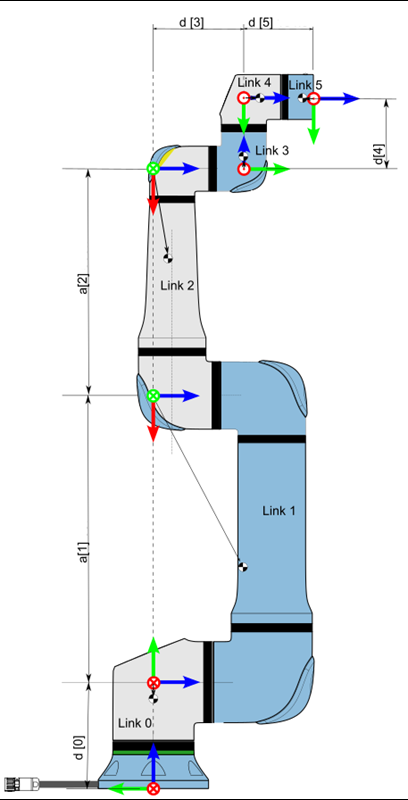
\includegraphics[width=0.4\textwidth]{figures/content/ur-dhmodel.png}
  \caption{D-H参数定义示意图}
  \label{fig:dh_parameters}
\end{figure}

\begin{table}[htbp]
  \centering
  \caption{标准D-H参数定义}
  \label{tab:dh_parameters}
  \begin{tabular}{cl}
    \toprule
    参数 & 定义 \\
    \midrule
    $a_{i-1}$ & 沿 $x_{i-1}$ 轴，从 $z_{i-1}$ 移动到 $z_i$ 的距离 \\
    $\alpha_{i-1}$ & 绕 $x_{i-1}$ 轴，从 $z_{i-1}$ 旋转到 $z_i$ 的角度 \\
    $d_i$ & 沿 $z_i$ 轴，从 $x_{i-1}$ 移动到 $x_i$ 的距离 \\
    $\theta_i$ & 绕 $z_i$ 轴，从 $x_{i-1}$ 旋转到 $x_i$ 的角度 \\
    \bottomrule
  \end{tabular}
\end{table}

根据D-H参数的定义，从坐标系\{i-1\}到坐标系\{i\}的变换可以分解为四次基本变换的乘积，其对应的齐次变换矩阵 $A_i$ 如式\ref{eq:dh_transform}所示。

\begin{equation}
  \label{eq:dh_transform}
  \begin{aligned}
    A_i &= \text{Rot}_{z, \theta_i} \text{Trans}_{z, d_i} \text{Trans}_{x, a_{i-1}} \text{Rot}_{x, \alpha_{i-1}} \\
        &= \begin{bmatrix}
          \cos\theta_i & -\sin\theta_i\cos\alpha_{i-1} & \sin\theta_i\sin\alpha_{i-1} & a_{i-1}\cos\theta_i \\
          \sin\theta_i & \cos\theta_i\cos\alpha_{i-1} & -\cos\theta_i\sin\alpha_{i-1} & a_{i-1}\sin\theta_i \\
          0 & \sin\alpha_{i-1} & \cos\alpha_{i-1} & d_i \\
          0 & 0 & 0 & 1
        \end{bmatrix}
  \end{aligned}
\end{equation}

通过为机械臂的每个连杆建立D-H参数表，即可得到从 $i=1$ 到 $n$ 的所有变换矩阵 $A_i$，为后续的正向与逆向运动学求解奠定数学基础。

\subsection{机械臂正逆向运动学求解}
\label{subsec:fk_ik_solution}

运动学求解旨在建立关节空间与笛卡尔空间之间的映射关系，是实现机械臂控制的核心。本小节将分别介绍正向运动学与逆向运动学求解的通用方法，为后续针对具体机械臂的分析提供理论框架。

正向运动学旨在根据已知的机械臂各关节变量，计算出末端执行器相对于基坐标系的位姿。通过D-H参数法建立的各连杆变换矩阵，这一过程可以通过将从基座到末端的连续变换矩阵 $A_i$ 依次相乘得到。对于一个 $n$ 自由度的机械臂，其末端执行器坐标系 \{n\} 相对于基坐标系 \{0\} 的总变换矩阵 $T_n^0$ 可由式\ref{eq:forward_kinematics}计算得出。

\begin{equation}
  \label{eq:forward_kinematics}
  T_n^0 = A_1(\theta_1) A_2(\theta_2) \cdots A_n(\theta_n)
\end{equation}

最终得到的 $T_n^0$ 矩阵中的旋转部分和平移部分即分别对应末端执行器的姿态和位置。正向运动学模型是唯一的，即一组给定的关节变量只能对应一个确定的末端位姿。

逆向运动学是正向运动学的逆问题，即根据给定的末端执行器在笛卡尔空间中的期望位姿，反向求解出满足该位姿的一组或多组关节变量。与正向运动学不同，逆向运动学的求解过程更为复杂，其解可能不唯一、存在多组解，或者在机械臂工作空间之外无解。逆向运动学的求解方法主要分为解析法和数值法两类。

解析法，也称代数法或几何法，通过对方程组 $T_n^0$ 进行代数运算或利用机械臂的几何关系来直接求解关节变量的封闭解。该方法计算速度快、能够求出所有可能的解，但仅适用于结构相对简单的机械臂，例如具有球形腕关节的六自由度机械臂。对于结构复杂的冗余机械臂，解析法通常难以适用。

数值法是一种迭代求解方法，它将逆向运动学问题转化为一个非线性优化问题。该方法从一个初始的关节角配置出发，通过迭代计算来逐步减小当前末端位姿与期望位姿之间的误差，直至误差小于预设阈值。基于雅可比矩阵的迭代法是其中最常用的一种，其核心思想如式\ref{eq:jacobian_inverse}所示。

\begin{equation}
  \label{eq:jacobian_inverse}
  \Delta\theta = J^{-1} \Delta x
\end{equation}

其中，$\Delta x$ 是末端位姿误差，$\Delta\theta$ 是关节角度的修正量，$J$ 是描述末端执行器速度与关节速度之间线性关系的雅可比矩阵。数值法通用性强，适用于任意结构的机械臂，但其计算量较大，可能陷入局部最优，且解的精度和收敛速度依赖于初始值的选取和迭代算法的设计。

\subsection{具体机械臂运动学求解}
\label{subsec:specific_robot_kinematics}

本节将前述理论应用于本研究后续实验所采用的 Franka Emika Panda 与 Universal Robots UR5 两款机械臂，对其运动学模型进行具体分析与求解。

Franka Emika Panda 是一款七自由度的冗余机械臂，其结构紧凑、灵活性高，广泛应用于学术研究。本研究的仿真实验将基于该款机械臂展开。根据其官方文档及相关研究，其改进D-H参数如表\ref{tab:panda_dh_parameters}所示。

\begin{table}[htbp]
  \centering
  \caption{Franka Panda 机械臂改进D-H参数}
  \label{tab:panda_dh_parameters}
  \begin{tabular}{ccccc}
    \toprule
    关节 $i$ & 连杆扭转角 $\alpha_{i-1}$ (rad) & 连杆长度 $a_{i-1}$ (m) & 连杆偏距 $d_i$ (m) & 关节角 $\theta_i$ (rad) \\
    \midrule
    1 & 0 & 0 & 0.333 & $\theta_1$ \\
    2 & $-\pi/2$ & 0 & 0 & $\theta_2$ \\
    3 & $\pi/2$ & 0 & 0.316 & $\theta_3$ \\
    4 & $\pi/2$ & 0.0825 & 0 & $\theta_4$ \\
    5 & $-\pi/2$ & -0.0825 & 0.384 & $\theta_5$ \\
    6 & $\pi/2$ & 0 & 0 & $\theta_6$ \\
    7 & $\pi/2$ & 0.088 & 0.107 & $\theta_7$ \\
    \bottomrule
  \end{tabular}
\end{table}

将表\ref{tab:panda_dh_parameters}中的参数代入式\ref{eq:dh_transform}，即可得到各关节的变换矩阵 $A_i$。例如，前两个关节的变换矩阵如式\ref{eq:panda_A1A2}所示。

\begin{equation}
\label{eq:panda_A1A2}
\begin{aligned}
A_1 &= \begin{bmatrix} c_1 & -s_1 & 0 & 0 \\ s_1 & c_1 & 0 & 0 \\ 0 & 0 & 1 & d_1 \\ 0 & 0 & 0 & 1 \end{bmatrix}, \quad
A_2 = \begin{bmatrix} c_2 & 0 & -s_2 & 0 \\ s_2 & 0 & c_2 & 0 \\ 0 & -1 & 0 & 0 \\ 0 & 0 & 0 & 1 \end{bmatrix}
\end{aligned}
\end{equation}

其中 $c_i = \cos\theta_i, s_i = \sin\theta_i$。其余各关节变换矩阵可同理求得。将所有变换矩阵连乘即可得到其正向运动学解 $T_7^0 = A_1 A_2 A_3 A_4 A_5 A_6 A_7$。由于 Franka Panda 是七自由度冗余机械臂，其逆运动学不存在封闭解析解，通常采用基于雅可比矩阵的数值法进行求解，利用其冗余自由度来优化关节限制、避开奇异点或执行次级任务。


Universal Robots UR5 是一款经典的六自由度协作机械臂，本研究的实物实验平台将采用该款机械臂。根据其官方文档，其标准D-H参数如表\ref{tab:ur5_dh_parameters}所示。

\begin{table}[htbp]
  \centering
  \caption{UR5 机械臂标准D-H参数}
  \label{tab:ur5_dh_parameters}
  \begin{tabular}{ccccc}
    \toprule
    关节 $i$ & 连杆扭转角 $\alpha_{i-1}$ (rad) & 连杆长度 $a_{i-1}$ (m) & 连杆偏距 $d_i$ (m) & 关节角 $\theta_i$ (rad) \\
    \midrule
    1 & $\pi/2$ & 0 & 0.089159 & $\theta_1$ \\
    2 & 0 & -0.42500 & 0 & $\theta_2$ \\
    3 & 0 & -0.39225 & 0 & $\theta_3$ \\
    4 & $\pi/2$ & 0 & 0.10915 & $\theta_4$ \\
    5 & $-\pi/2$ & 0 & 0.09465 & $\theta_5$ \\
    6 & 0 & 0 & 0.08230 & $\theta_6$ \\
    \bottomrule
  \end{tabular}
\end{table}

UR5 机械臂的腕部三轴交于一点，满足 Pieper 准则，因此其逆运动学存在封闭的解析解。求解过程采用解析法，通过解耦思想将位置和姿态问题分开处理。该方法首先通过求解腕部中心点的位置来确定前三个关节 $\theta_1, \theta_2, \theta_3$ 的值，随后基于已求出的前三个关节的姿态来解算后三个腕部关节 $\theta_4, \theta_5, \theta_6$。具体推导过程如下：

给定末端期望位姿矩阵 $T_6^0 = \begin{bmatrix} R & p \\ 0 & 1 \end{bmatrix} = \begin{bmatrix} n_x & o_x & a_x & p_x \\ n_y & o_y & a_y & p_y \\ n_z & o_z & a_z & p_z \\ 0 & 0 & 0 & 1 \end{bmatrix}$，腕部中心点 $p_c$ 的位置可以通过从末端点 $p$ 沿末端坐标系 $z_6$ 轴的反方向平移 $d_6$ 得到：

\begin{equation}
  p_c = p - d_6 \cdot R \cdot \begin{bmatrix} 0 \\ 0 \\ 1 \end{bmatrix} = \begin{bmatrix} p_x - d_6 a_x \\ p_y - d_6 a_y \\ p_z - d_6 a_z \end{bmatrix}
\end{equation}

关节角 $\theta_1$ 的求解涉及到将 $p_c$ 投影到 $x_0-y_0$ 平面。从俯视角度看，$p_c$ 的投影点、基座原点以及关节2的轴线构成一个三角形，通过反正切函数和余弦定理即可求解。$\theta_1$ 通常存在两组解，对应机械臂左手和右手两种不同的构型：

\begin{equation}
  \theta_1 = \text{arctan2}(p_{cy}, p_{cx}) - \text{arctan2}(d_4, \pm\sqrt{p_{cx}^2 + p_{cy}^2 - d_4^2})
\end{equation}

关节角 $\theta_5$ 的求解利用了变换矩阵的特性。将总变换方程 $T_6^0 = T_1^0 T_2^1 T_3^2 T_4^3 T_5^4 T_6^5$ 左乘 $(T_1^0)^{-1}$，得到 $T_6^1 = (T_1^0)^{-1} T_6^0$。展开该矩阵的对应元素，可以发现它仅与 $\theta_5$ 有关，从而得到 $\theta_5$ 的两组解：

\begin{equation}
  \theta_5 = \pm \text{arccos}\left(\frac{p_x s_1 - p_y c_1 - d_4}{d_6}\right)
\end{equation}

关节角 $\theta_6$ 可在求出 $\theta_5$ 后，通过 $T_6^1$ 矩阵的旋转部分元素得到。当 $\sin\theta_5 \neq 0$ 时，即非奇异位形下：

\begin{equation}
  \theta_6 = \text{arctan2}\left(\frac{-o_x s_1 + o_y c_1}{\sin\theta_5}, \frac{n_x s_1 - n_y c_1}{\sin\theta_5}\right)
\end{equation}

关节角 $\theta_3$ 的求解同样利用几何关系。在关节2和关节3所在的平面内，连杆 $a_2$ 和 $a_3$ 与 $p_c$ 在该平面上的投影构成一个三角形。利用余弦定理可得：

\begin{equation}
  \theta_3 = \pm \text{arccos}\left(\frac{\|p_{c}\|^2 - d_1^2 - d_4^2 - a_2^2 - a_3^2}{2 a_2 a_3}\right)
\end{equation}

关节角 $\theta_2$ 可由 $\theta_1$ 和 $\theta_3$ 共同确定。其求解涉及到求解一个关于 $\sin\theta_2$ 和 $\cos\theta_2$ 的线性方程组，最终可表示为：

\begin{equation}
  \theta_2 = \text{arctan2}(-p_{cz}, \pm\sqrt{p_{cx}^2+p_{cy}^2-d_4^2}) - \text{arctan2}(a_3 s_3, a_2 + a_3 c_3)
\end{equation}

最后，关节角 $\theta_4$ 可由旋转矩阵 $R_3^6 = (R_3^0)^{-1} R_6^0$ 的元素得到，其中 $R_3^0$ 由已求出的前三个关节角确定：

\begin{equation}
  \theta_4 = \text{arctan2}(R_{3,2}^6, R_{3,1}^6)
\end{equation}

由于三角函数的周期性和对称性，UR5 的逆运动学通常存在八组不同的关节角配置，均能使末端达到同一位姿。该解析解能够计算出所有可能的关节角配置，为实时控制提供了确定性的解集。

\section{模仿学习理论}
\label{sec:imitation_learning}

\subsection{模仿学习原理}
\label{subsec:il_principles}

模仿学习的核心目标是让智能体通过观察专家的示范数据，隐式地学习并内化专家的行为策略，从而使其在面对相似的状态与场景时，能够自主做出与专家一致的决策。与高度依赖奖励函数工程和大量试错探索的强化学习相比，模仿学习能够更自然、更高效地从人类直觉操作中提取高维任务特征，极大降低了策略学习的样本复杂度与安全风险。

在模仿学习的理论框架中，机械臂与环境的交互过程通常被建模为离散时间的部分可观察马尔可夫决策过程。该过程可以用一个多元组 $\mathcal{M} = \langle \mathcal{S}, \mathcal{A}, \mathcal{P}, \mathcal{R}, \Omega, \mathcal{O}, \gamma, \rho_0 \rangle$ 来进行形式化定义。具体而言，$\mathcal{S}$ 表示系统的真实状态空间，在机械臂任务中通常包含机械臂各关节的绝对角度、末端执行器的物理开合状态以及环境中物体的真实位姿；$\mathcal{A}$ 表示动作空间，定义了智能体能够执行的连续控制指令集合，例如关节的角速度或轴角目标位置；$\mathcal{P}(s_{t+1}|s_t, a_t)$ 是环境的状态转移概率分布，描述了在状态 $s_t$ 下执行动作 $a_t$ 后系统状态演化的动力学机制。由于传感器噪声和视觉遮挡，机械臂无法获取完整的真实状态，只能获得观测空间 $\Omega$ 中的观测值 $o_t$，这一过程由观测概率分布 $\mathcal{O}(o_t|s_t)$ 决定。$\mathcal{R}(s_t, a_t)$ 为潜在的真实奖励函数，而模仿学习的根本特征即在于不依赖与环境交互来获取此显式奖励；$\gamma$ 为折扣因子，$\rho_0(s_1)$ 则是初始状态分布。

在标准设定中，假定存在一个具有极高任务完成率的专家策略，表示为条件概率分布 $\pi_E(a|s)$。在训练阶段，算法接收一组由专家提供的演示轨迹集合 $\mathcal{D} = \{\tau_1, \tau_2, \dots, \tau_N\}$。其中，每一条轨迹 $\tau_i$ 记录了从初始状态到终止状态的完整序列交互，可表示为 $\tau_i = \{(o_1, a_1), (o_2, a_2), \dots, (o_T, a_T)\}$。模仿学习的最终目的，是在给定的参数化策略空间中，寻找一个由神经网络参数化的最优策略 $\pi_\theta(a|o)$，使其最大程度地逼近专家策略。

传统行为克隆是模仿学习中最基础且应用最为广泛的方法。它将序列决策学习过程直接转化为一个标准的监督学习问题，摒弃了对时间依赖性和环境动力学的假设。在概率论视角下，行为克隆的目标是最大化专家演示数据在参数化策略下的对数似然期望。其优化目标可表述为：

\begin{equation}
  \theta^* = \arg\max_\theta \mathbb{E}_{(o,a) \sim \mathcal{D}} \left[ \log \pi_\theta(a|o) \right]
\end{equation}

在实际的机械臂连续控制任务中，动作空间是连续且高维的。若假设学习到的策略服从各向同性的高斯分布，即 $\pi_\theta(a|o) = \mathcal{N}(\mu_\theta(o), \Sigma)$，其中均值 $\mu_\theta(o)$ 由深度神经网络输出，$\Sigma = \sigma^2 I$ 为固定的协方差矩阵。根据高斯分布的概率密度函数，最大化对数似然目标可以等价转换为最小化网络预测动作与专家真实动作之间的均方误差：

\begin{equation}
  \mathcal{L}_{\text{BC}}(\theta) = \frac{1}{|\mathcal{D}|} \sum_{(o,a) \in \mathcal{D}} \| a - \mu_\theta(o) \|^2
\end{equation}

尽管行为克隆凭借其算法实现上的简单性与直接性，在诸多视觉控制任务中取得了初步成功，但其独立同分布的强假设在马尔可夫决策过程中是失效的。当机械臂根据当前学习到的策略在物理环境中实际执行动作时，其当前时刻微小的预测误差会不可避免地改变下一时刻的环境状态，从而破坏了测试时状态分布与训练时专家状态分布的一致性。这种由微小误差引发的连锁反应，正是限制行为克隆在复杂任务中应用的核心理论瓶颈。为了突破这一瓶颈，近期的研究转向利用长序列依赖建模和动作空间扩展，通过从根本上改变动作预测的时域结构来延缓甚至消除这种误差累积。
\subsection{典型模仿学习算法}
\label{subsec:typical_il_algorithms}

在解决精细操作任务的模仿学习问题时，动作分块 Transformer 算法（Action Chunking with Transformers, ACT）\cite{zhao2023learning} 表现出了优异的性能。该算法基于 Transformer 架构构建了条件变分自编码器的编码器和解码器，用于对示教数据进行建模。具体而言，编码器负责对输入数据进行处理并高效提取关键特征；解码器则先借助 ResNet 网络对图像进行编码，随后通过 Transformer 编码器将多模态特征深度融合，最终由 Transformer 解码器生成连贯、流畅的动作序列。

针对模仿学习中存在的误差累积和人类演示非平稳问题，ACT 采用了动作分块策略。该策略将连续的动作序列分割为多个相对独立的动作组块，有效减少了误差在动作执行过程中的传递与积累。在面对高精度控制和闭环反馈的精细操作任务时，ACT 策略会预测未来 $k$ 个时间步的动作，使得任务的有效视野降低 $k$ 倍，以此缓解误差累积问题。

此外，为提升策略的平滑性，ACT 引入了时间集成机制。在每个时间步推理动作序列时，生成不同时刻的动作组块，并按时序排列使不同动作组块相互重叠。在任一时间步生成多个预测动作后，采用指数加权平均的方式组合这些预测：

\begin{equation}
  w_i = \exp(-m \cdot i)
\end{equation}

其中 $w_0$ 是初始动作的权重，$m$ 为权重系数。这种加权组合机制进一步优化了动作生成的连贯性。

% \begin{figure}[htbp]
%   \centering
%   \includegraphics[width=0.6\textwidth]{figures/content/[此处需要补充具体数据/文献/细节]}
%   \caption{基于 Transformer 的 ACT 模仿学习框架}
%   \label{fig:act_architecture}
% \end{figure}

尽管 ACT 算法在精细操作任务中成效显著，但其在处理复杂动作分布和高维动作空间能力上仍有不足，难以执行复杂手部动作。相比之下，扩散策略算法（Diffusion Policy）\cite{chi2023diffusion} 能够在处理复杂动作分布时精准生成合适策略，高效探索高维动作空间并寻得最优解，且具备出色的训练稳定性。

扩散策略基于去噪扩散概率模型，以随机朗之万动力学为理论基础，将动作序列的生成视为去噪过程。传统的显式策略将世界状态直接映射到动作，在处理多模态行为时存在局限；隐式策略通过能量函数定义动作分布，虽能表示多模态分布但训练时需负采样导致过程不稳定。扩散策略则不直接输出动作，而是基于视觉观察推断动作分数的梯度，并通过迭代逐步优化动作。这使其能够自然精确地表达多模态动作分布，适应高维动作空间，并通过直接学习能量函数梯度避免了传统负采样的不稳定问题。

在具体原理上，扩散策略的输出生成过程被建模为去噪过程。在第 $k$ 次迭代中，去噪公式如下：

\begin{equation}
  x^{k-1} = \alpha \left( x^k - \gamma \epsilon_\theta(x^k, k) + \mathcal{N}(0, \sigma^2 I) \right)
\end{equation}

其中，$\epsilon_\theta(x^k, k)$ 是噪声预测网络，通过学习不断优化以准确预测噪声；$\alpha$、$\gamma$ 和 $\sigma$ 是与迭代步骤 $k$ 相关的参数，共同构成噪声调度；$\mathcal{N}(0, \sigma^2 I)$ 是每次迭代添加的高斯噪声，为迭代引入随机性以避免陷入局部最优。训练时，通过最小化均方误差损失函数来训练噪声预测网络：

\begin{equation}
  L = \text{MSE} \left( \epsilon^k, \epsilon_\theta(x^0 + \epsilon^k, k) \right)
\end{equation}

为适应机械臂任务，扩散策略在视觉观察条件设定方面进行了改进，使用扩散模型近似条件分布以加快扩散过程。给定时间步 $t$ 的观察数据 $O_t$，预测动作序列 $A_t$ 的去噪过程具体为：

\begin{equation}
  A_t^{k-1} = \alpha \left( A_t^k - \gamma \epsilon_\theta(O_t, A_t^k, k) + \mathcal{N}(0, \sigma^2 I) \right)
\end{equation}

相应的训练损失公式为：

\begin{equation}
  L = \text{MSE} \left( \epsilon^k, \epsilon_\theta(O_t, A_t^0 + \epsilon^k, k) \right)
\end{equation}

% \begin{figure}[htbp]
%   \centering
%   \includegraphics[width=0.6\textwidth]{figures/content/[此处需要补充具体数据/文献/细节]}
%   \caption{不同策略表示方法对比及 Diffusion Policy 算法框架}
%   \label{fig:diffusion_policy_architecture}
% \end{figure}

在闭环动作序列预测上，扩散策略将动作序列预测能力与滚动时域控制相结合。在时间步 $t$，以最近 $T_o$ 步的观察数据为输入，预测 $T_p$ 步的动作，其中前 $T_a$ 步的动作会被直接执行在机械臂上而无需重新规划。这种设计平衡了长期规划与实时响应。

在网络架构设计上，扩散策略采用 CNN 和 Transformer 架构进行构建。基于 CNN 的架构使用修改后的 1D 时间卷积网络，借助 FiLM 预测动作轨迹；基于 Transformer 的架构则凭借输入与注意力机制，在高复杂度任务中表现卓越。具体而言，采用 ResNet18 作为视觉编码器，以空间 Softmax 池化替换全局平均池化以保留图像空间信息；用 GroupNorm 替代 BatchNorm 并与指数移动平均相结合，有效保障了训练稳定性。通过噪声调度合理调控扩散过程中的噪声变化，助力模型捕捉动作信号的高频和低频特征，从而优化动作生成的准确性与稳定性。

\section{视觉语言动作模型}
\label{sec:vla_models}

[此处需要补充视觉语言动作模型相关内容]

\chapter{基于扩散模型的模仿学习动作生成算法}
\label{chp:diffusion_action_generation}

在机械臂操作任务中，由于环境的复杂性和任务的多样性，同一任务往往存在多条合理的操作路径，这种现象导致专家示教数据中的动作分布呈现出明显的多模态特性。传统的行为克隆方法通常假设动作分布是单峰的，倾向于将多种可能的动作轨迹平均化，这在面临多模态分布时容易产生无效甚至危险的动作指令。为了解决这一问题，本章提出一种基于扩散模型的模仿学习动作生成算法，利用扩散模型对复杂数据分布的拟合能力，提升动作策略在非结构化环境中的适应性和鲁棒性，并在机器人操作数据集RoboMimic\cite{mandlekar2021matters}上进行验证。

\section{扩散动作生成算法}
\label{sec:diffusion_action_architecture}

基于扩散模型的模仿学习动作生成算法的核心在于构建一个能够融合多模态感知信息并输出连续动作序列的条件生成模型。该算法的整体架构如图\ref{fig:action_model}所示，主要由特征编码器、特征融合模块和扩散动作生成模块三部分组成。

\begin{figure}[htbp]
  \centering
  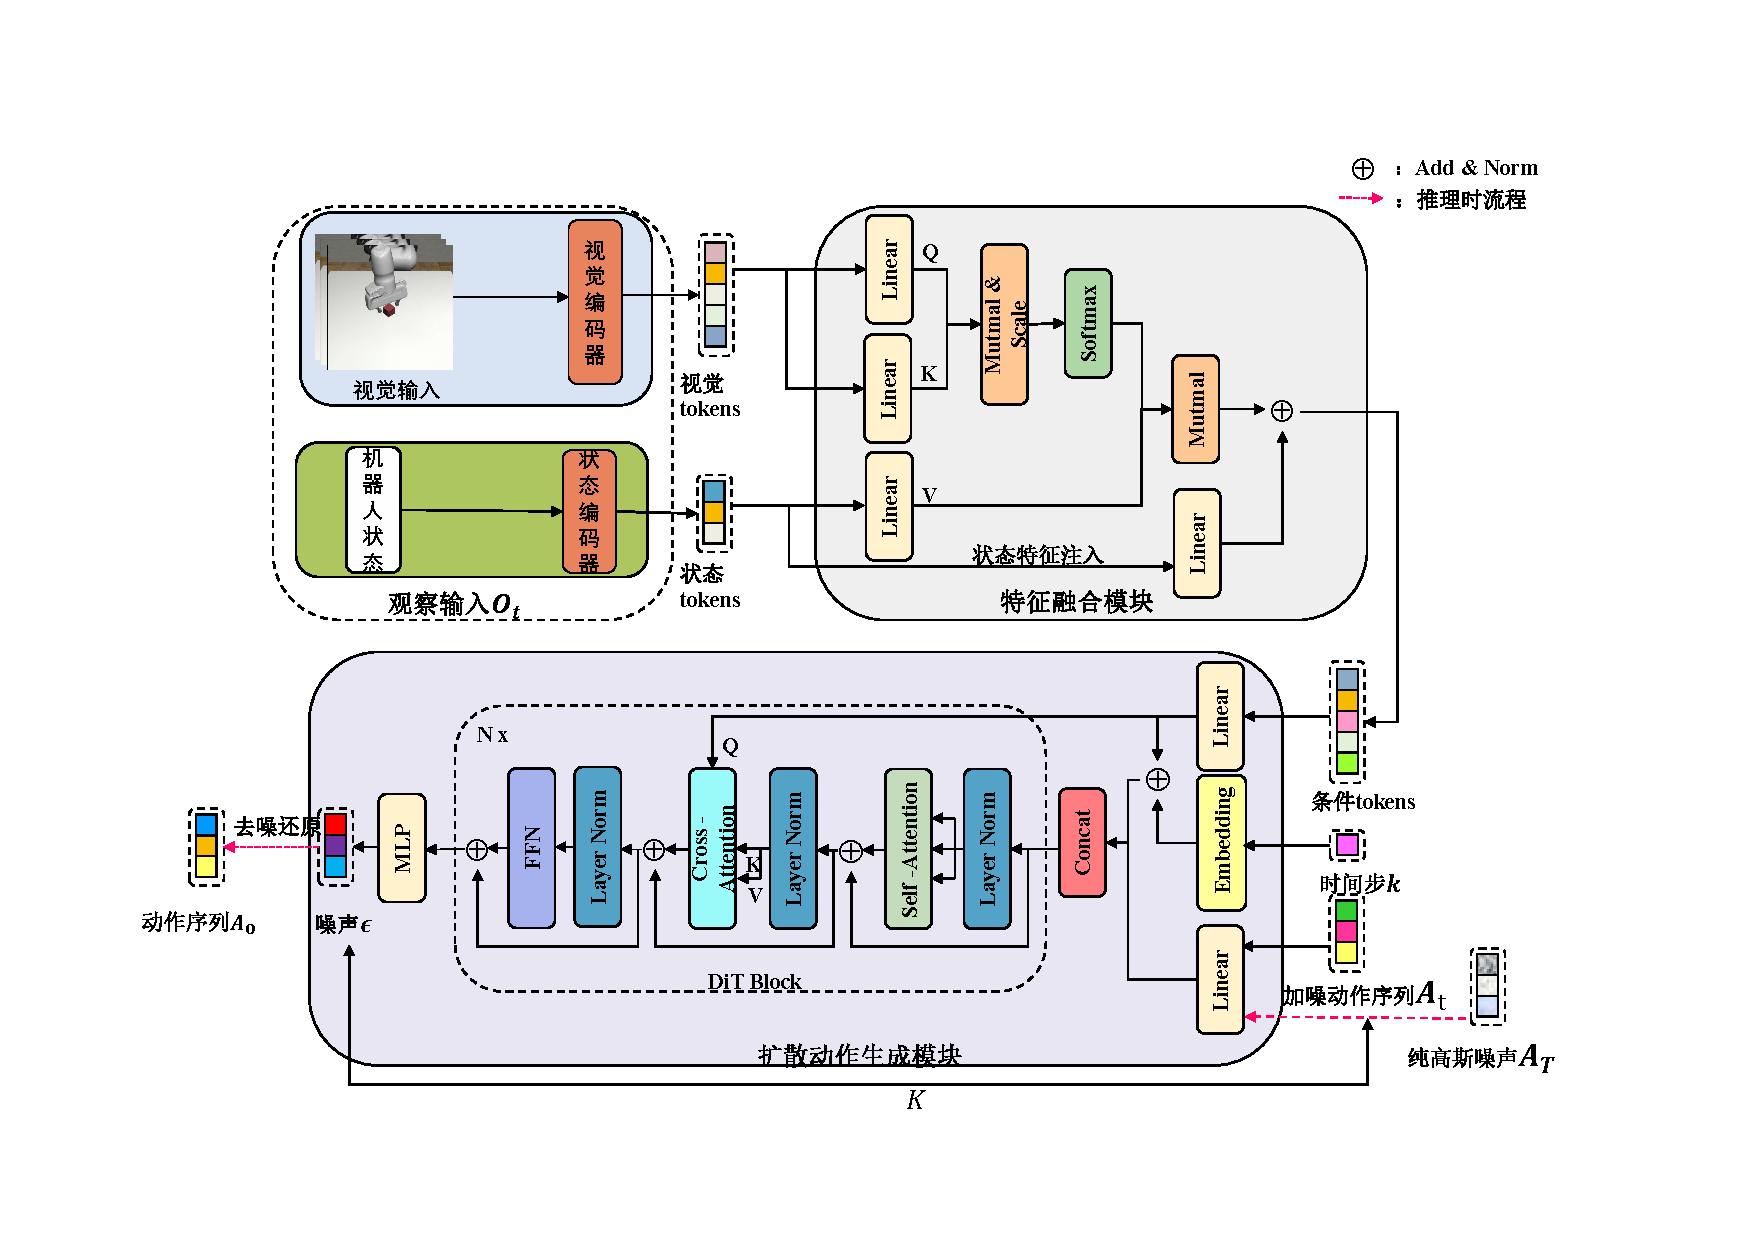
\includegraphics[width=0.88\linewidth]{figures/content/action_model}
  \caption{基于扩散模型的模仿学习动作生成算法整体架构}
  \label{fig:action_model}
\end{figure}

系统首先接收来自环境的观察输入 $O_t$，该输入包含视觉输入和机器人状态两部分，视觉输入通过视觉编码器提取为视觉特征表示，而机器人当前关节角度、末端执行器位姿等状态，则通过状态编码器转化为状态特征表示。这两种特征表示在特征融合模块中进行交互与整合，以形成统一的条件特征,为后续的动作生成提供充分的环境与自身状态上下文。

扩散动作生成模块负责基于上述条件特征生成连续的动作序列 $A_0$,该模块采用基于Transformer架构的扩散模型（DiT）\cite{peebles2023scalable}作为核心去噪网络，DiT网络由多个堆叠的DiT Block组成，用于逐步预测输入序列中的噪声 $\epsilon$。在训练阶段，模型接收添加了噪声的动作序列 $A_t$、当前时间步 $k$ 以及条件特征作为输入。在推理阶段，模型从纯高斯噪声出发，在条件特征的引导下，经过多步迭代去噪，最终生成符合专家分布的干净动作序列 $A_0$，并下发给机械臂执行。

\subsection{视觉与状态特征编码}
\label{sec:visual_state_encoding}
在本文提出的基于扩散模型的动作生成算法中，模型需要结合多步的历史观察序列来预测未来的动作序列。由于每一时间步的视觉观测都需要经过编码器处理，计算延迟和显存占用会随着观察窗口步数的增加而线性增长。如果在视觉编码阶段产生过高的延迟或占用过多的显存，将严重制约整个动作生成算法的实时性。为了在保证特征提取质量的同时满足机械臂实时控制对推理速度的要求，本算法采用EfficientViT\cite{cai2023efficientvit}作为视觉编码器的骨干网络，传统的视觉Transformer通常依赖于标准的Softmax自注意力机制来获取全局感受野，但其计算复杂度和显存消耗与输入图像分辨率的平方成正比。这在处理高分辨率的多帧图像序列时，会带来不可接受的计算负担。EfficientViT通过引入多尺度线性注意力机制，在保持全局感受野和多尺度学习能力的同时，降低了计算复杂度和内存消耗，从而能够契合了本算法对高效视觉编码的需求。


\begin{figure}[htbp]
  \centering
  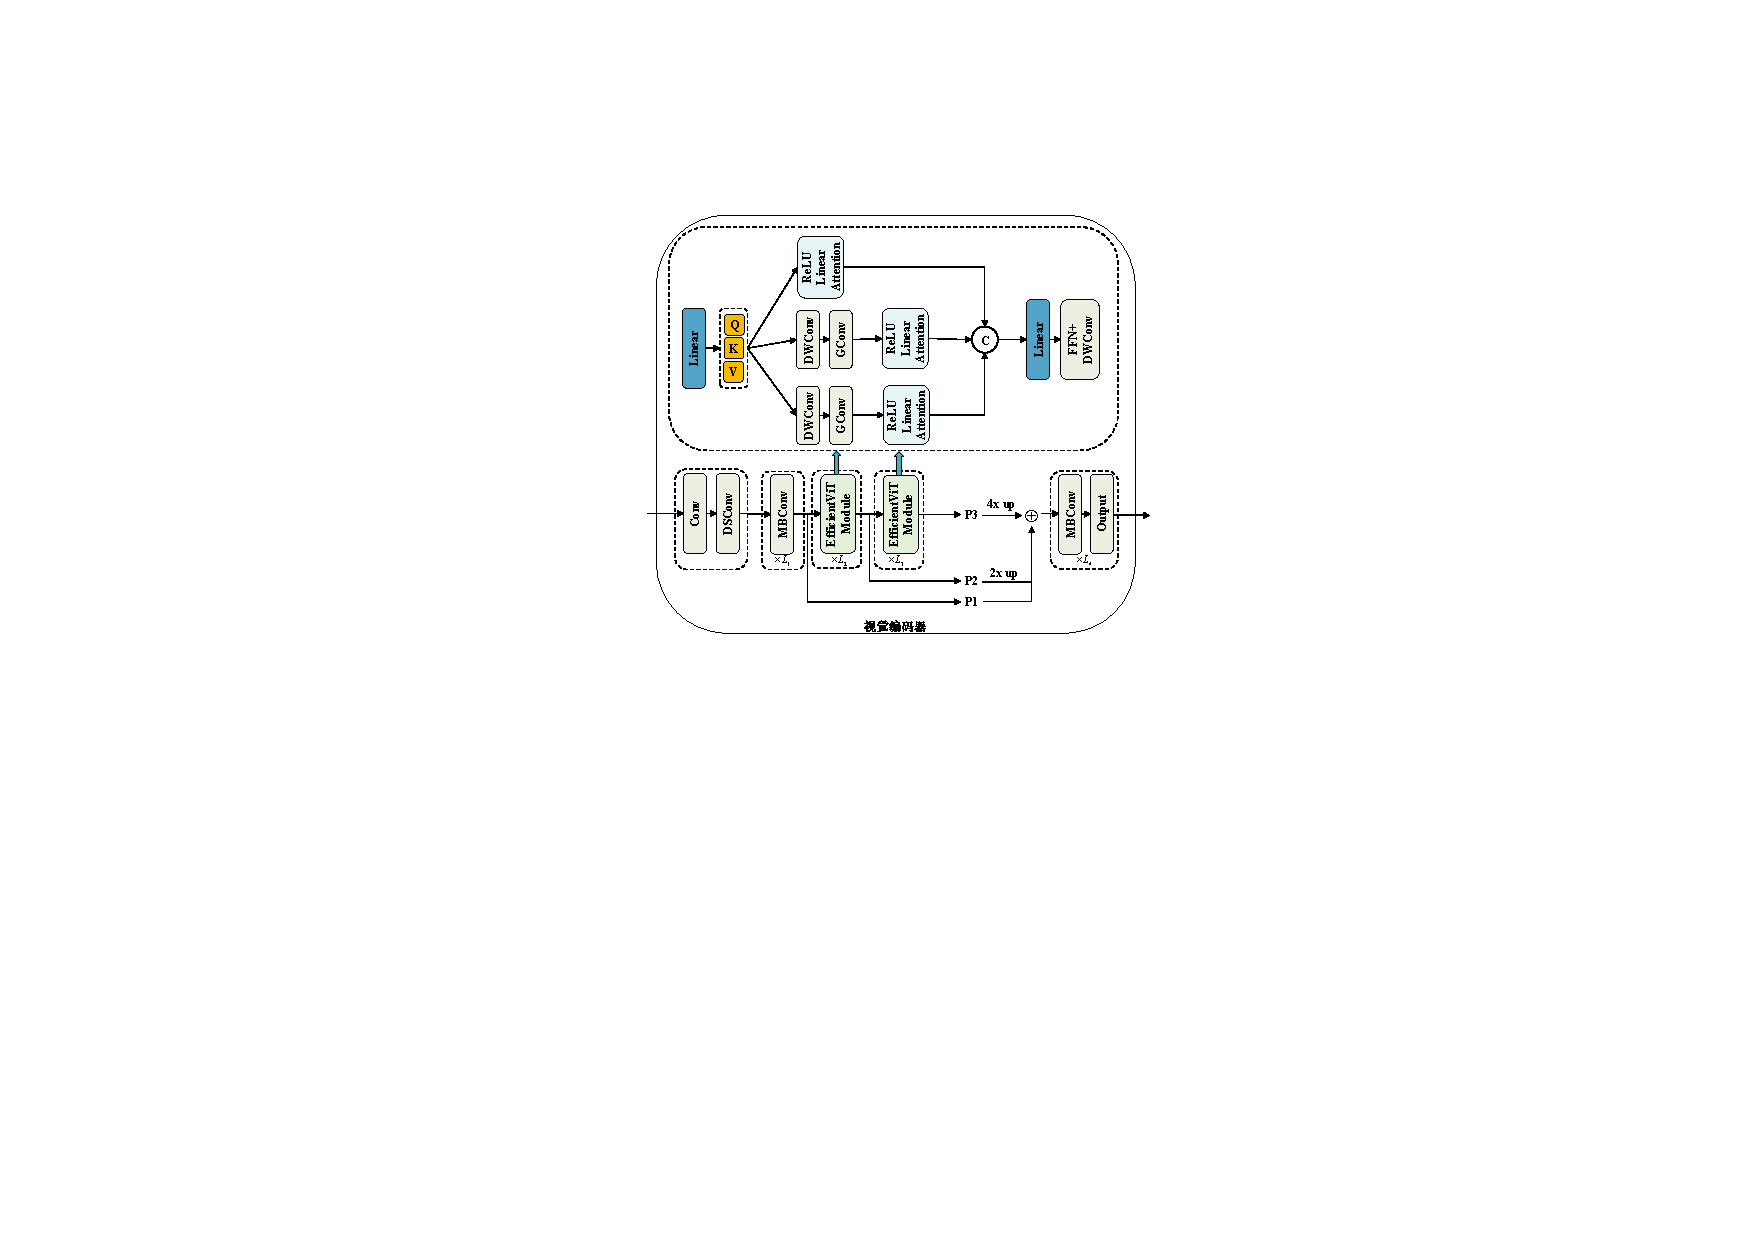
\includegraphics[width=0.8\linewidth]{figures/content/efficent_vit}
  \caption{EfficientViT视觉编码器网络结构}
  \label{fig:efficient_vit}
\end{figure}

如图\ref{fig:efficient_vit}所示，EfficientViT视觉编码器通过多阶段的网络结构对输入图像进行层次化的特征提取。网络设计中广泛采用了轻量化卷积操作，其中DSConv表示深度可分离卷积，MBConv表示移动翻转瓶颈卷积，DWConv表示深度卷积，GConv表示组卷积。在初始阶段，输入图像经过普通卷积和深度可分离卷积进行初步的下采样和特征提取。随后，特征图进入包含EfficientViT模块的核心处理阶段。

EfficientViT模块内部采用轻量级的多尺度注意力机制，特征首先经过线性层映射为Q、K和V向量。为了克服传统线性注意力在局部信息提取上的不足，模块利用不同分组的深度可分离卷积和组卷积对Q、K、V向量进行局部聚合，生成多尺度特征表示。随后，模块采用ReLU激活函数替代传统的Softmax函数进行注意力计算，通过利用矩阵乘法的结合律，ReLU线性注意力将计算顺序从先计算注意力权重矩阵转变为先计算键和值的乘积，从而将计算复杂度从与分辨率的平方级关系降低为线性关系。此外，使用ReLU替代Softmax避免了在硬件上执行效率低下的行归一化操作，大幅提升了内存访问效率。

多尺度注意力图在通道维度上进行拼接后，再通过线性层进行特征融合。同时，网络在不同阶段之间引入了上采样操作，以便在不同分辨率层级之间进行特征融合，从而捕获丰富的空间细节和全局语义信息。这种机制上的协同配合，使得EfficientViT在提取高质量视觉特征的同时，大幅降低了多步观察序列带来的显存压力和计算延迟。最终，视觉编码器输出一组具有高表征能力的视觉特征向量，用于后续的特征融合与动作生成。

对于机器人状态编码，由于各关节的当前角度、末端执行器位姿和夹爪的开合状态这样的状态数据通常是低维向量，可直接采用多层感知机（MLP）作为状态编码器，如图\ref{fig:state_encoder}。该编码器由两个全连接层和GeLU激活函数组成，负责将低维的原始状态向量映射到与视觉特征相同维度的高维潜在空间中，并通过Position Embedding得到状态向量，以便在特征融合模块中与视觉特征进行有效的交互和对齐。
\begin{figure}[htbp]
  \centering
  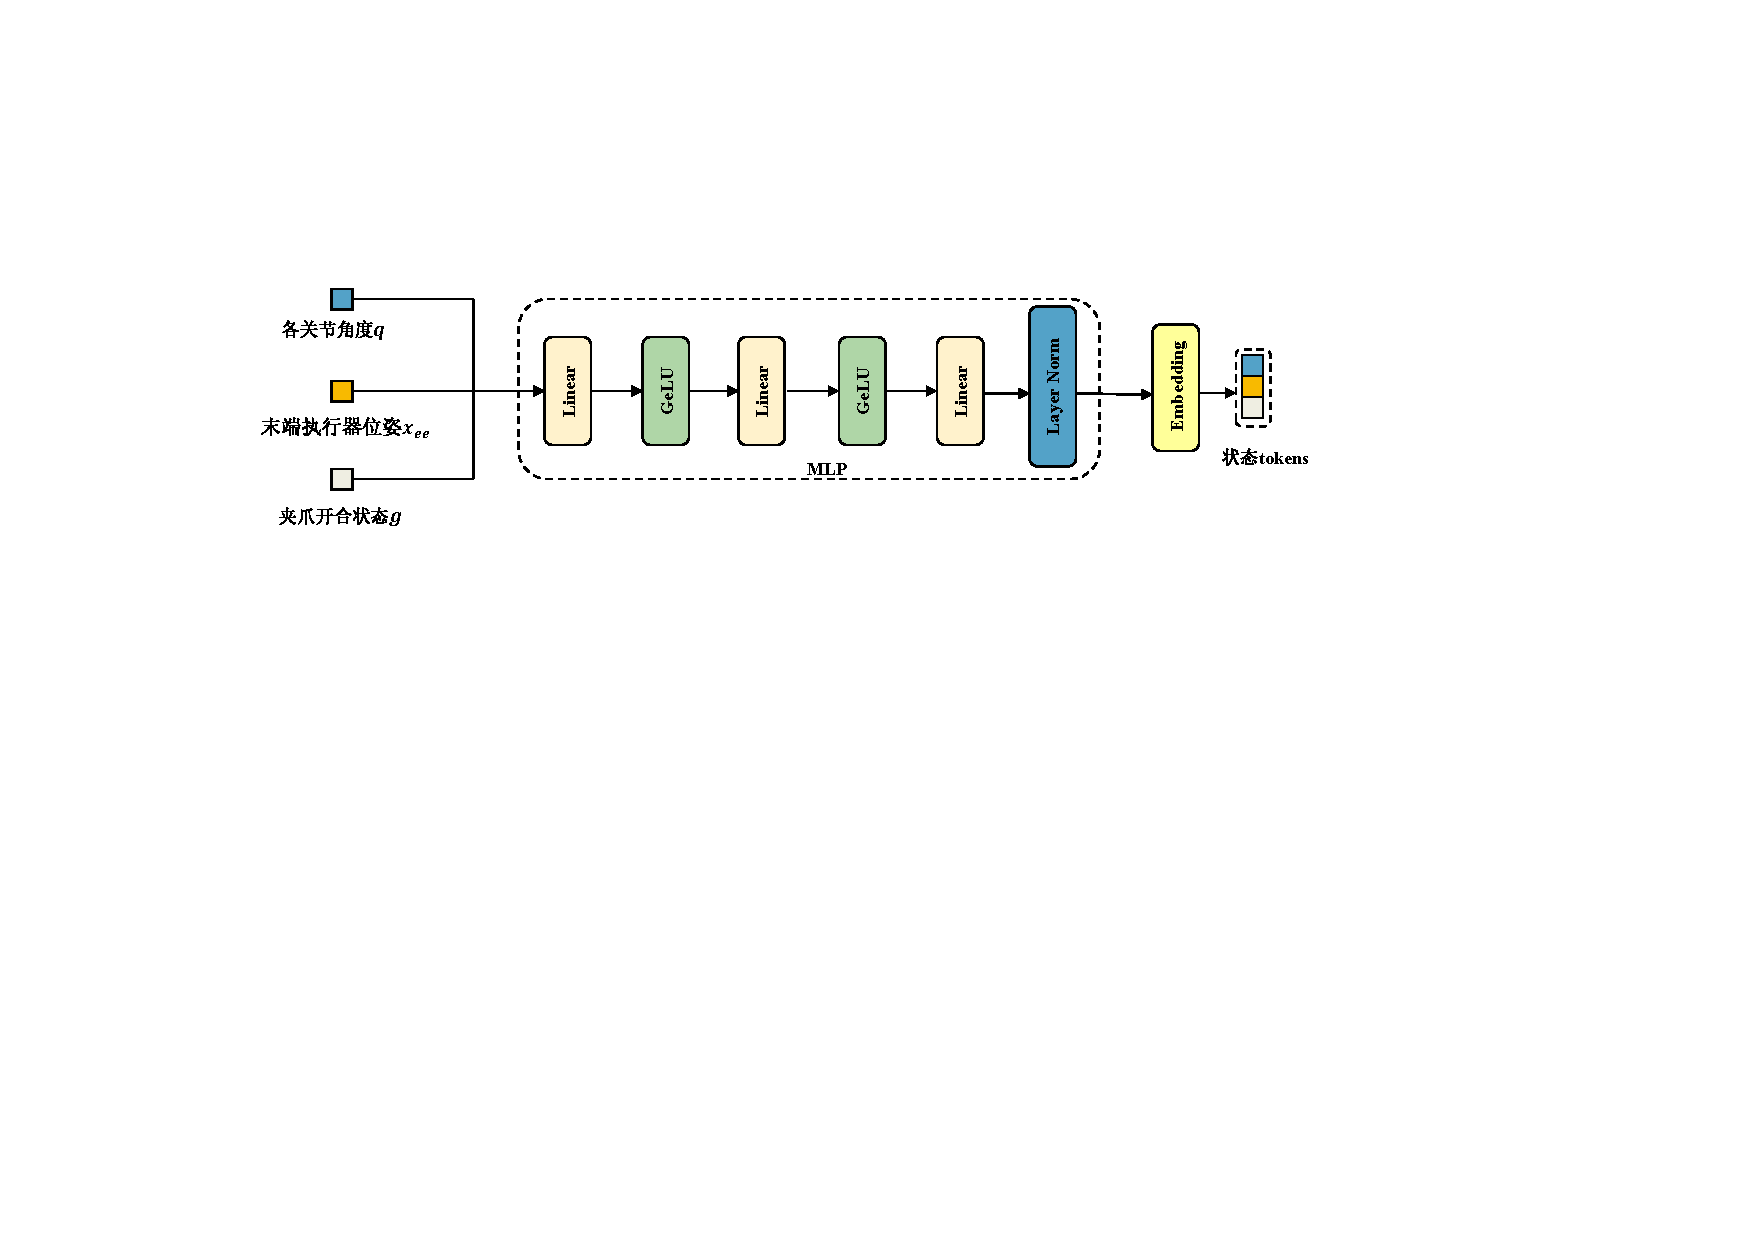
\includegraphics[width=0.66\linewidth]{figures/content/state_encoder}
  \caption{状态编码器结构示意图}
  \label{fig:state_encoder}
\end{figure}



\chapter{基于特征时序缓存的视觉语言动作模型}
\label{chp:temporal_cache_vla}

\section{引言}
\label{sec:chap4_intro}

在第三章中，本文提出了一种基于扩散模型的视觉语言动作生成框架，通过跨模态注意力机制实现了视觉特征与本体状态的有效融合，并在单步动作生成任务中展现了优异的性能。然而，在真实的非结构化环境中，机器人操作任务往往具有长视距和时序依赖的特性。例如，在执行“按下按钮”等操作时，动作前后的视觉观测几乎没有差异，如果仅依赖当前单帧图像进行决策，模型极易产生“动作是否已经完成”的混淆，从而导致重复操作或任务失败。这种现象凸显了机器人操作任务本质上具有的非马尔可夫特性，即当前的决策不仅依赖于当前的观测，还需要结合历史的上下文信息。

为了解决上述长时序任务中的决策依赖问题，本章在第三章所提出的扩散动作生成模型的基础上，进一步引入了时序缓存机制，提出了一种基于特征时序缓存的视觉语言动作模型（TemporalCacheVLA）。该模型受到人类认知科学中双重记忆系统的启发，通过构建感知-语义双通道历史存储池，有效地保存和提取长视野中的低维感知细节与高维认知语义。本章将详细阐述TemporalCacheVLA框架的整体设计、视觉语言特征感知模块、时序缓存机制，以及如何将提取的时序特征接入前文所述的扩散动作生成模型中。最后，通过在LIBERO长时序任务基准上的对比实验与消融实验，系统地验证所提方法的有效性。

\section{TemporalCacheVLA框架整体设计}
\label{sec:chap4_framework}

人类在执行复杂操作任务时，通常依赖于工作记忆（Working Memory）和情景记忆（Episodic Memory）的协同作用。工作记忆负责短暂保留当前信息以供即时决策，而情景记忆则负责长期存储过去的经验细节与抽象语义。受此启发，TemporalCacheVLA框架被设计为一个“感知-存储-动作”的闭环系统，其整体架构如图~\ref{fig:temporal_cache_vla_arch}~所示。

\begin{figure}[htbp]
  \centering
  % TODO: 替换为真实的TemporalCacheVLA整体架构图路径
  \includegraphics[width=0.95\linewidth]{figures/content/temporal_cache_vla_arch}
  \caption{TemporalCacheVLA框架整体架构图}
  \label{fig:temporal_cache_vla_arch}
\end{figure}

TemporalCacheVLA框架主要由三个核心模块构成：
\begin{enumerate}
  \item \textbf{视觉语言特征感知模块}：负责接收当前的RGB图像观测与自然语言指令，利用预训练的视觉编码器和大语言模型提取细粒度的感知特征（Perceptual Tokens）和高层次的认知语义特征（Cognitive Tokens），形成当前时刻的工作记忆。
  \item \textbf{感知-语义双通道历史存储池}：作为情景记忆的载体，该模块包含感知和认知两个独立的存储通道。在每个时间步，工作记忆会通过交叉注意力机制从存储池中检索相关的历史上下文，并通过门控机制与当前特征进行自适应融合。同时，存储池会根据相似度对冗余信息进行合并压缩，以维持长时序下的紧凑表示。
  \item \textbf{基于时序缓存的扩散动作生成模块}：将融合了历史时序上下文的感知与认知特征作为条件输入，接入第三章所提出的扩散动作生成模型中。通过迭代去噪过程，生成具有时序连贯性的未来多步动作序列。
\end{enumerate}

通过上述设计，TemporalCacheVLA不仅继承了扩散模型在拟合复杂多模态动作分布方面的优势，还赋予了模型在长视距任务中理解时序依赖关系的能力。

\section{视觉语言特征感知与时序缓存机制}
\label{sec:chap4_perception_memory}

\subsection{视觉语言特征感知}
\label{subsec:chap4_perception}

在每个时间步 $t$，机器人接收当前的RGB图像观测 $I_t \in \mathbb{R}^{H \times W \times 3}$ 和自然语言指令 $L$。为了充分提取图像中的空间细节与语义信息，本文采用了双分支的视觉编码架构。具体而言，使用预训练的DINOv2\cite{oquab2023dinov2}和SigLIP\cite{zhai2023sigmoid}作为视觉主干网络，分别提取图像的局部纹理特征和全局语义特征。

提取到的原始视觉特征经过一个基于Squeeze-and-Excitation（SE）瓶颈层的感知压缩模块，被压缩为紧凑的感知特征序列 $p_t \in \mathbb{R}^{N_p \times d_p}$，其中 $N_p$ 为特征序列长度，$d_p$ 为特征维度。与此同时，原始视觉特征通过线性投影层映射到语言模型的嵌入空间中，并与分词后的语言指令拼接，输入到拥有70亿参数的大语言模型（如LLaMA\cite{touvron2023llama}）中。取大语言模型在句子结束符（EOS）位置的输出作为认知特征 $c_t \in \mathbb{R}^{1 \times d_c}$，该特征高度浓缩了当前场景的高层认知语义。

感知特征 $p_t$ 和认知特征 $c_t$ 共同构成了当前时刻的工作记忆 $M_{wk}$：
\begin{equation}
  M_{wk} = \{ p_t \in \mathbb{R}^{N_p \times d_p}, c_t \in \mathbb{R}^{1 \times d_c} \}
\end{equation}

\subsection{感知-语义双通道历史存储池}
\label{subsec:chap4_memory_pool}

为了克服单帧工作记忆缺乏时序依赖的缺陷，本文设计了感知-语义双通道历史存储池（Perceptual-Cognitive Memory Bank, PCMB）。该存储池 $M_{pcmb}$ 包含感知和认知两个通道，分别存储历史的感知细节与认知语义：
\begin{equation}
  M_{pcmb} = \{ m^x \mid x \in \{\text{per}, \text{cog}\} \}
\end{equation}
\begin{equation}
  m^x = \{ m_i^x \in \mathbb{R}^{N_x \times d_x} \}_{i=1}^L, \quad x \in \{\text{per}, \text{cog}\}
\end{equation}
其中，$L$ 为存储池的最大容量。

\textbf{记忆检索}：在每个时间步，当前的工作记忆 $M_{wk}$ 作为查询向量（Query），从存储池中检索相关的历史信息。为了保留历史特征的时序顺序，本文为存储池中的每个条目引入了正弦位置编码 $\text{TE}(\cdot)$。以感知通道为例，检索过程的键（Key）和值（Value）构建如下：
\begin{equation}
  K^x = [m_1^x + \text{TE}(t_1); \dots; m_L^x + \text{TE}(t_L)], \quad V^x = [m_1^x; \dots; m_L^x]
\end{equation}
随后，通过缩放点积注意力机制计算检索结果 $H^x$：
\begin{equation}
  H^x = \text{softmax}\left( \frac{q^x (K^x)^\top}{\sqrt{d_x}} \right) V^x, \quad q^x \in \{p_t, c_t\}, \quad x \in \{\text{per}, \text{cog}\}
\end{equation}

\textbf{门控融合}：检索到的历史特征 $H^x$ 需要与当前特征 $x$ 进行融合。为了自适应地决定历史信息的保留程度，本文设计了一个基于多层感知机（MLP）的门控机制。门控向量 $g^x$ 的计算公式为：
\begin{equation}
  g^x = \sigma(\text{MLP}(\text{concat}[x, H^x]))
\end{equation}
其中 $\sigma$ 为Sigmoid激活函数。最终的融合特征 $\tilde{x}$ 为：
\begin{equation}
  \tilde{x} = g^x \odot H^x + (1 - g^x) \odot x
\end{equation}
其中 $\odot$ 表示逐元素相乘。

\textbf{记忆压缩与更新}：融合后的特征 $\tilde{x}$ 将被更新至存储池中。当存储池的条目数量超过容量 $L$ 时，系统会计算相邻条目之间的余弦相似度，并选取相似度最高的一对相邻条目进行平均池化合并，从而在保持紧凑表示的同时剔除冗余信息：
\begin{equation}
  i^* = \arg\max_{i=1,\dots,L-1} \cos(\tilde{x}_i, \tilde{x}_{i+1})
\end{equation}
\begin{equation}
  m_{i^*}^x \leftarrow \frac{1}{2}(\tilde{x}_{i^*} + \tilde{x}_{i^*+1})
\end{equation}

\section{基于时序缓存的扩散动作生成}
\label{sec:chap4_diffusion_action}

在获取了融合时序上下文的感知特征 $\tilde{p}$ 和认知特征 $\tilde{c}$ 后，本文将其作为条件信号，接入第三章所提出的扩散动作生成模型中。第三章详细论述了扩散模型在处理多模态动作分布时的优势，以及如何通过去噪过程生成平滑的动作轨迹。本节将重点阐述时序缓存特征与扩散模型的结合方式。

假设机器人需要预测未来 $T$ 步的动作序列 $A = (a_t, a_{t+1}, \dots, a_{t+T-1})$，其中每步动作 $a_i \in \mathbb{R}^7$ 包含三维平移、三维旋转（欧拉角）以及一维的夹爪开闭状态。在扩散模型的训练阶段，真实的动作序列 $A^0$ 被逐步添加高斯噪声，生成一系列带有噪声的动作序列 $A^k$（$k \in [1, K]$ 为扩散步数）。

在去噪推理阶段，模型需要根据条件信号从纯噪声 $A^K$ 中逐步恢复出清晰的动作序列 $A^0$。本文将认知特征 $\tilde{c}$ 作为高层语义引导，将感知特征 $\tilde{p}$ 作为细粒度视觉补充。具体而言，在扩散模型的每一次去噪迭代中，噪声动作序列 $A^k$ 首先与当前去噪步数 $k$ 的正弦位置编码相加，然后与认知特征 $\tilde{c}$ 在序列维度上拼接。随后，拼接后的特征输入到基于Transformer的去噪网络中。在Transformer的交叉注意力层中，感知特征 $\tilde{p}$ 作为键（Key）和值（Value），为动作去噪提供精确的空间对齐信息。

去噪网络的优化目标是最小化预测动作与真实动作之间的均方误差（MSE）：
\begin{equation}
  \mathcal{L} = \mathbb{E}_{k, A^0, \epsilon \sim \mathcal{N}(0,I)} \left[ \| \epsilon - \epsilon_\theta(A^k, \tilde{p}, \tilde{c}, k) \|^2 \right]
\end{equation}
其中 $\epsilon_\theta$ 为去噪网络预测的噪声。通过这种方式，第三章的扩散动作生成模型被无缝集成到TemporalCacheVLA框架中，使其不仅具备了强大的多模态动作拟合能力，还获得了处理长时序依赖的全局视野。

\section{实验与分析}
\label{sec:chap4_experiments}

\subsection{实验设置}
\label{subsec:chap4_exp_setup}

为了全面评估TemporalCacheVLA在长时序和复杂操作任务中的性能，本文选取了具有高度挑战性的LIBERO\cite{liu2023libero}机器人操作基准数据集进行仿真实验。LIBERO是一个专门用于评估机器人终身学习与知识迁移能力的大规模基准，其包含了丰富的任务变体和复杂的环境交互。

LIBERO数据集共包含五个子集，分别侧重于评估机器人操作能力的不同维度：
\begin{enumerate}
  \item \textbf{LIBERO-Spatial（空间子集）}：包含10个任务，主要测试机器人在不同空间布局下的推理与操作能力，例如在不同位置抓取特定物体。
  \item \textbf{LIBERO-Object（物体子集）}：包含10个任务，侧重于评估模型对不同视觉外观、形状和纹理的物体的泛化能力。
  \item \textbf{LIBERO-Goal（目标子集）}：包含10个任务，要求机器人在相同的初始场景下，根据不同的语言指令完成不同的目标状态。
  \item \textbf{LIBERO-Long（长时序子集）}：包含10个任务，是数据集中最具挑战性的部分。该子集要求机器人执行包含多个子目标的复杂长序列操作，例如“打开抽屉，将碗放入抽屉，然后关闭抽屉”。这类任务极度依赖历史上下文信息，是验证本文时序缓存机制有效性的理想测试床。
  \item \textbf{LIBERO-90（综合子集）}：包含90个多样化的任务，全面考察模型在海量任务中的综合表现与容量极限。
\end{enumerate}

在实验中，每个任务包含50条人类专家示教轨迹。本文的模型仅使用第三人称视角的单帧RGB图像和自然语言指令作为输入，不依赖任何腕部相机视图或本体感受状态（如关节角度、末端位姿等）。模型在8张NVIDIA A100 GPU上进行训练，批大小设置为256，学习率为 $2 \times 10^{-5}$。在推理阶段，采用DDIM\cite{ho2020denoising}加速采样算法，去噪步数设置为10步。

\subsection{对比实验结果与分析}
\label{subsec:chap4_comparison}

为了验证TemporalCacheVLA的先进性，本文将其与当前领域内的主流视觉语言动作模型进行了全面的对比，包括Diffusion Policy\cite{chi2023diffusion}、Octo\cite{team2024octo}、OpenVLA\cite{kim2024openvla}、TraceVLA\cite{zheng2024tracevla}、CogACT\cite{liang2024cogact}以及$\pi_0$\cite{black2024pi}等。各方法在LIBERO五个子集上的成功率对比结果如表~\ref{tab:libero_results}~所示。

\begin{table}[htbp]
  \centering
  \caption{不同方法在LIBERO基准数据集上的成功率对比（\%）}
  \label{tab:libero_results}
  \resizebox{\textwidth}{!}{
  \begin{tabular}{lcccccc}
    \toprule
    方法 & Spatial & Object & Goal & Long & LIBERO-90 & 平均成功率 \\
    \midrule
    Diffusion Policy\cite{chi2023diffusion} & 78.3 & 92.5 & 68.3 & 50.5 & - & 72.4 \\
    Octo\cite{team2024octo} & 78.9 & 85.7 & 84.6 & 51.1 & - & 75.1 \\
    MDT\cite{reuss2024mdt} & 78.5 & 87.5 & 73.5 & 64.8 & - & 76.1 \\
    UniACT\cite{zheng2025uniact} & 77.0 & 87.0 & 77.0 & 70.0 & 73.0 & 76.8 \\
    MaIL\cite{jia2024mail} & 74.3 & 90.1 & 81.8 & 78.6 & - & 83.5 \\
    SpatialVLA\cite{qu2025spatialvla} & 88.2 & 89.9 & 78.6 & 55.5 & 46.2 & 71.7 \\
    TraceVLA\cite{zheng2024tracevla} & 84.6 & 85.2 & 75.1 & 54.1 & - & 74.8 \\
    OpenVLA\cite{kim2024openvla} & 84.7 & 88.4 & 79.2 & 53.7 & 73.5 & 75.9 \\
    CoT-VLA\cite{zhao2025cotvla} & 87.5 & 91.6 & 87.6 & 69.0 & - & 81.1 \\
    $\pi_0$-FAST\cite{pertsch2025pi0fast} & 96.4 & 96.8 & 88.6 & 60.2 & 83.1 & 85.0 \\
    TriVLA\cite{liu2025trivla} & 91.2 & 93.8 & 89.8 & 73.2 & - & 87.0 \\
    4D-VLA\cite{zhang2025_4dvla} & 88.9 & 95.2 & 90.9 & 79.1 & - & 88.6 \\
    CogACT\cite{liang2024cogact} & 97.2 & 98.0 & 90.2 & 88.8 & 92.1 & 93.2 \\
    $\pi_0$\cite{black2024pi} & 96.8 & 95.8 & 95.8 & 85.2 & - & 94.2 \\
    \midrule
    \textbf{TemporalCacheVLA (本文)} & \textbf{98.0} & \textbf{98.1} & \textbf{95.9} & \textbf{92.2} & \textbf{94.9} & \textbf{95.8} \\
    \bottomrule
  \end{tabular}
  }
\end{table}

从表~\ref{tab:libero_results}~的数据可以看出，本文提出的TemporalCacheVLA在所有子集上均取得了优异的表现，平均成功率达到了$95.8\%$，显著超越了OpenVLA（$75.9\%$）和Octo（$75.1\%$）等主流基线模型。特别值得注意的是，在最具挑战性的LIBERO-Long长时序子集上，传统缺乏时序建模的方法（如OpenVLA和Diffusion Policy）成功率仅在$50\%$左右徘徊，而TemporalCacheVLA将成功率大幅提升至$92.2\%$。这一结果强有力地证明了感知-语义双通道历史存储池在捕捉长视野时序依赖方面的关键作用。

此外，在包含90个任务的LIBERO-90综合子集上，TemporalCacheVLA同样取得了$94.9\%$的高成功率，优于CogACT的$92.1\%$和$\pi_0$-FAST的$83.1\%$。这表明本文方法不仅在处理长时序任务时具有优势，在面对大规模、多样化的任务分布时，依然能够保持强大的泛化能力和策略稳定性。

\subsection{消融实验}
\label{subsec:chap4_ablation}

为了深入分析TemporalCacheVLA中各个核心组件对整体性能的贡献，本文在长时序任务上进行了详细的消融实验。实验主要考察了时序缓存机制中记忆通道的选择、记忆检索方式以及记忆融合策略的影响。

\begin{enumerate}
  \item \textbf{记忆通道消融}：当仅使用认知语义通道时，模型能够理解任务的宏观进度，但在精细操作时容易产生偏差；当仅使用感知细节通道时，模型能够对齐空间位置，但容易在长序列中迷失当前的目标阶段。只有同时结合双通道记忆，模型才能在长时序任务中取得最佳的成功率。
  \item \textbf{位置编码消融}：在记忆检索阶段，如果去除时间步的正弦位置编码，模型将无法区分历史特征的先后顺序，导致在执行具有严格顺序要求的任务（如先开门再取物）时性能显著下降。
  \item \textbf{融合策略消融}：对比直接相加与门控融合两种策略，实验结果表明，门控机制能够更有效地过滤无关的历史噪声，自适应地提取对当前决策有用的上下文信息，从而带来更高的动作生成质量。
\end{enumerate}

\section{本章小结}
\label{sec:chap4_summary}

本章针对机器人长时序操作任务中的决策依赖问题，提出了一种基于特征时序缓存的视觉语言动作模型（TemporalCacheVLA）。该模型受人类双重记忆系统启发，设计了感知-语义双通道历史存储池，实现了对长视野中低维感知细节与高维认知语义的有效缓存与检索。同时，本章详细阐述了如何将提取的时序上下文特征作为条件信号，无缝接入第三章所提出的扩散动作生成模型中，从而赋予模型在复杂非马尔可夫环境下的全局视野与多模态动作生成能力。在LIBERO大规模基准数据集上的对比实验表明，TemporalCacheVLA在各项任务上均取得了领先的成功率，特别是在长时序任务子集上实现了显著的性能飞跃，充分验证了所提框架的有效性与先进性。

\chapter{基于GELLO遥操作的机器人系统集成与验证}
\label{chp:robot_system_integration}
算法在仿真环境中的有效性并不能直接保证其在真实场景下的可用性，感知噪声、通信延迟与机械误差等因素均会对模型的实际表现产生影响。将模仿学习算法部署至真实机械臂平台，需要解决数据采集、模型推理与底层控制之间的系统集成问题。本章搭建总体框架如图~\ref{fig:real_system_integration}~所示，基于GELLO~\cite{wu2024gello}遥操作装置的真实场景数据采集平台，设计模型推理服务的远端部署方案与基于机器人操作系统（Robot Operating System, ROS）的真机控制接口，并在真实操作任务上对前述算法进行实验验证，考察其在真实场景下的实际应用价值。

\begin{figure}
    \centering
    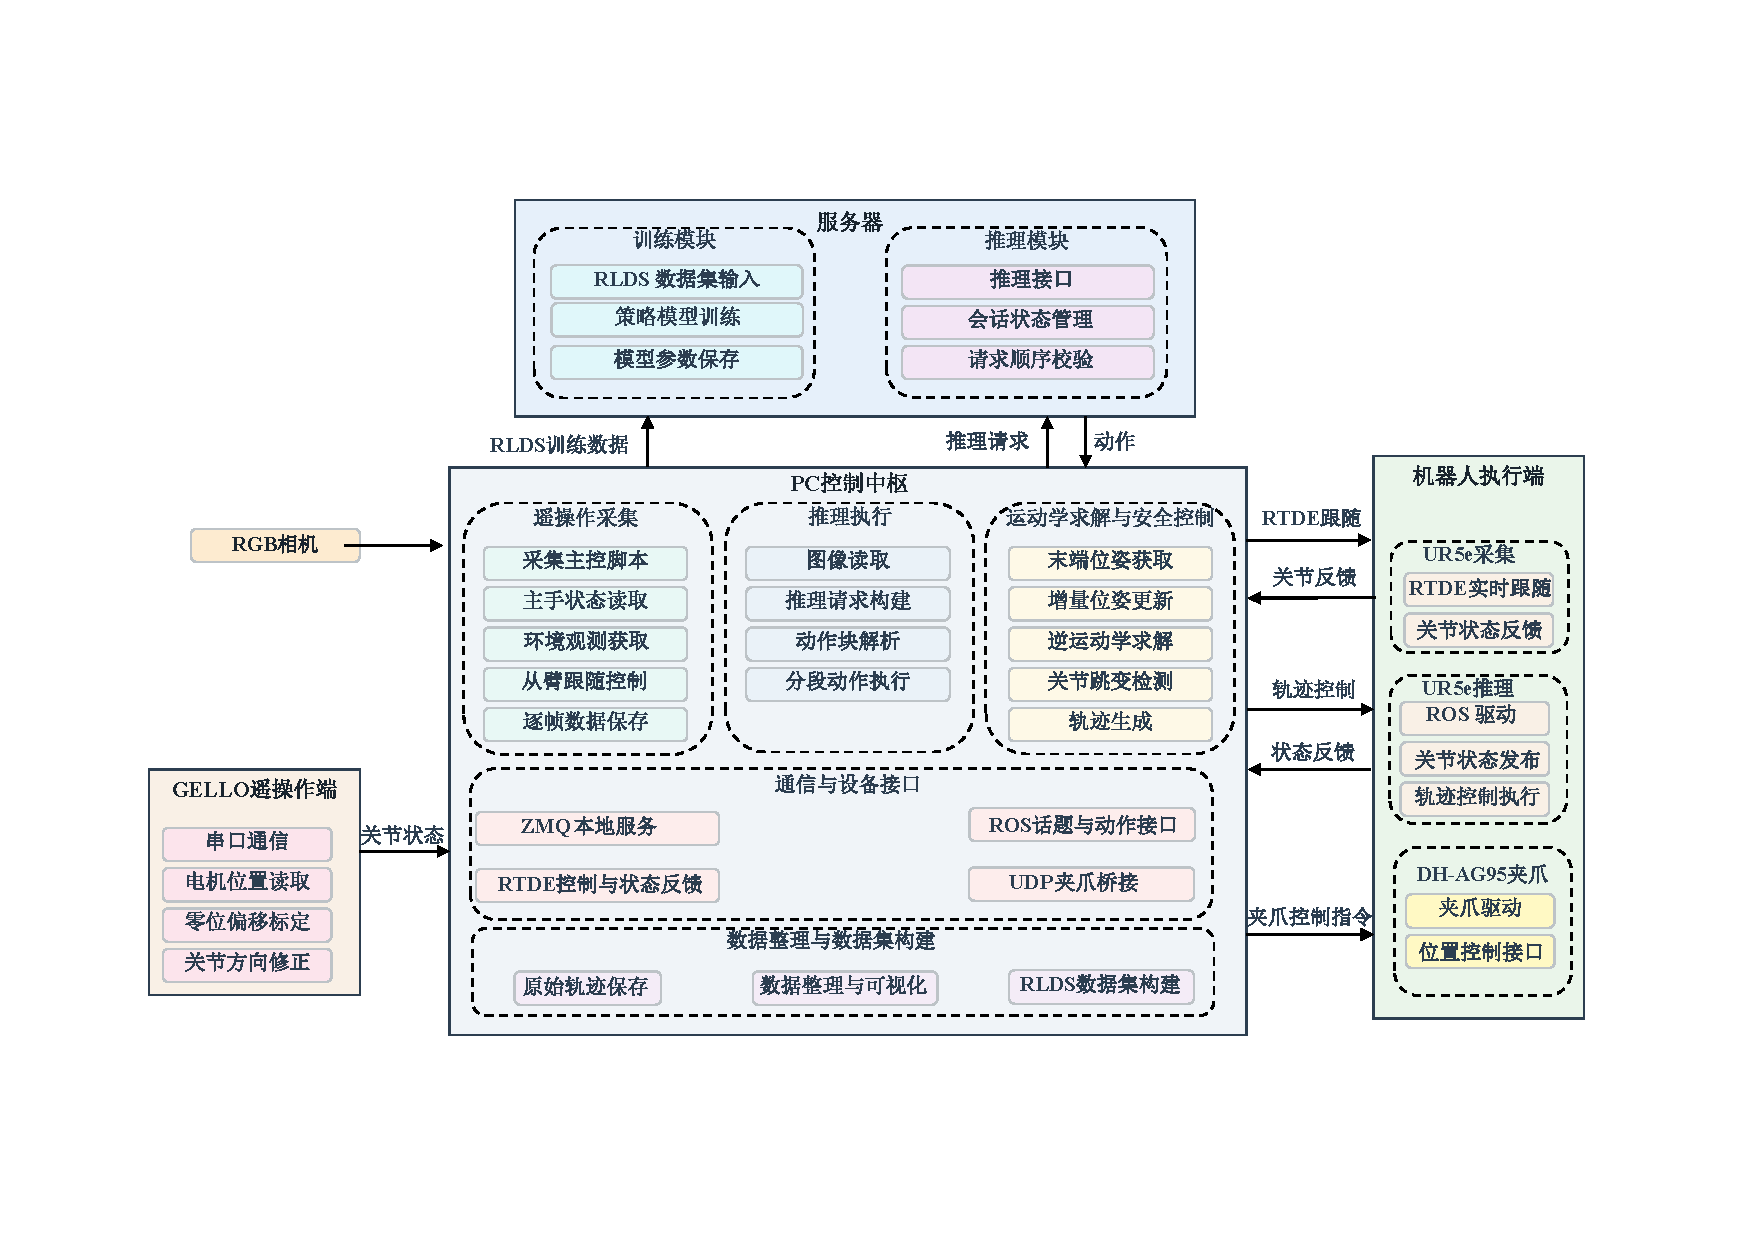
\includegraphics[width=0.95\linewidth]{figures/content/real_robot_system}
    \caption{基于GELLO遥操作装置的机器人系统集成框架示意图}
    \label{fig:real_system_integration}
\end{figure}

\section{GELLO遥操作装置与数据采集平台}
\label{sec:gello_teleop_platform}

在机器人模仿学习中，高质量的数据是训练有效策略的前提。由于前面提出的视觉语言动作模型都是通过扩散模型作为动作生成模型的，而扩散模型需要拟合具有多峰性的动作分布，传统的编程示教和拖动示教难以满足扩散模型对所学习数据的多峰性分布的要求。为了在真实环境中采集覆盖多种操作路径的模仿学习动作轨迹，本节采用遥操作作为数据采集的主要手段。这种方式使操作者能够通过自然的肢体运动直接驱动机械臂，所采集的轨迹天然覆盖多种操作路径，与扩散模型对多峰性数据分布的要求相契合；同时，遥操作装置在关节空间中与目标机械臂直接映射，采集到的关节角度与夹爪状态无需经过逆运动学转换，可直接作为模型的训练标签，避免了坐标变换引入的累积误差。

\subsection{GELLO遥操平台硬件构成}
\label{subsec:gello_hardware}

遥操作硬件设计的核心难点在于如何消除操作者与目标机械臂之间的运动学差异。为了实现关节空间的直接映射控制，遥操臂必须与目标机械臂具有相同的运动学结构。为此，本平台选用了GELLO开源框架，通过3D打印结构件与Dynamixel智能舵机，构建了与UR5e机械臂运动学等价的缩比遥操臂。由于遥操臂与目标机械臂共享相同的运动学结构，操作者在转动遥操臂时，目标机械臂的对应关节产生同步的角位移，操作者自身的运动便受到相同的关节限制约束，所采集的轨迹天然满足机械臂的运动学可行性要求。

参与数据采集的核心机电设备如图~\ref{fig:hardware_components}~所示。目标执行端采用UR5e六自由度协作机械臂，该机械臂具备5 kg的有效载荷与850 mm的最大工作半径，能够满足桌面级复杂操作任务的需求。末端执行器配备了大寰DH-AG95自适应平行夹爪，其最大开口宽度达到95 mm，满足多种物体的抓取需求。在感知端，系统部署了一个固定视角的RGB相机，用于捕获工作空间的图像信息。在控制端，GELLO遥操臂作为UR5e的缩比复制品，通过七个Dynamixel舵机实现对目标机械臂及末端夹爪的全状态控制。

\begin{figure}[htbp]
  \centering
  \subfloat[UR5e机械臂]{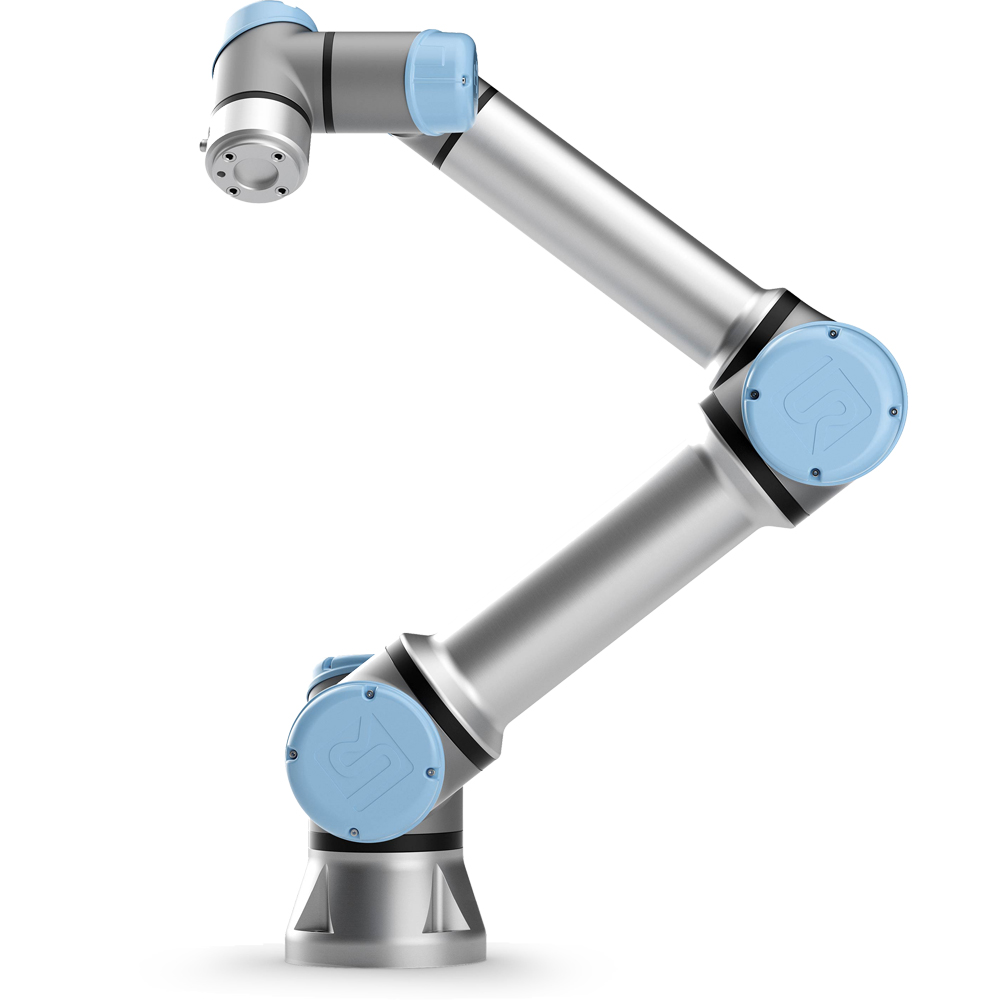
\includegraphics[width=.2\textwidth]{figures/content/UR5e.jpg}}
  \quad
  \subfloat[RGB相机]{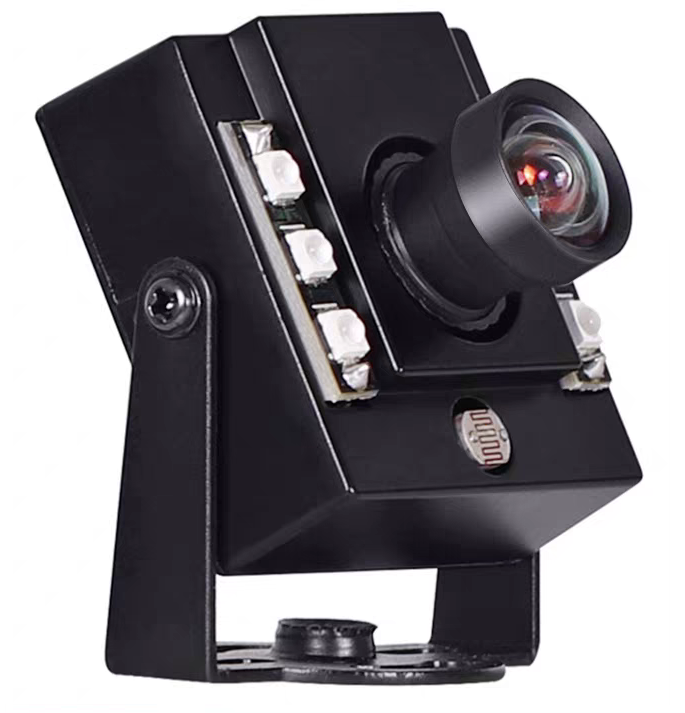
\includegraphics[width=.2\textwidth]{figures/content/camera_pic.png}}
  \\
  \subfloat[DH-AG95夹爪]{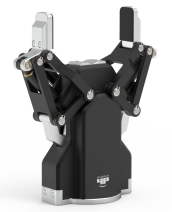
\includegraphics[width=.2\textwidth]{figures/content/dh-ag95.png}}
  \quad
  \subfloat[Dynamixel舵机]{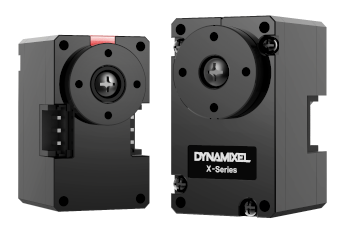
\includegraphics[width=.2\textwidth]{figures/content/dynamixel.png}}
  \caption{参与数据采集的核心机电设备}
  \label{fig:hardware_components}
\end{figure}

\begin{figure}[htbp]
  \centering
  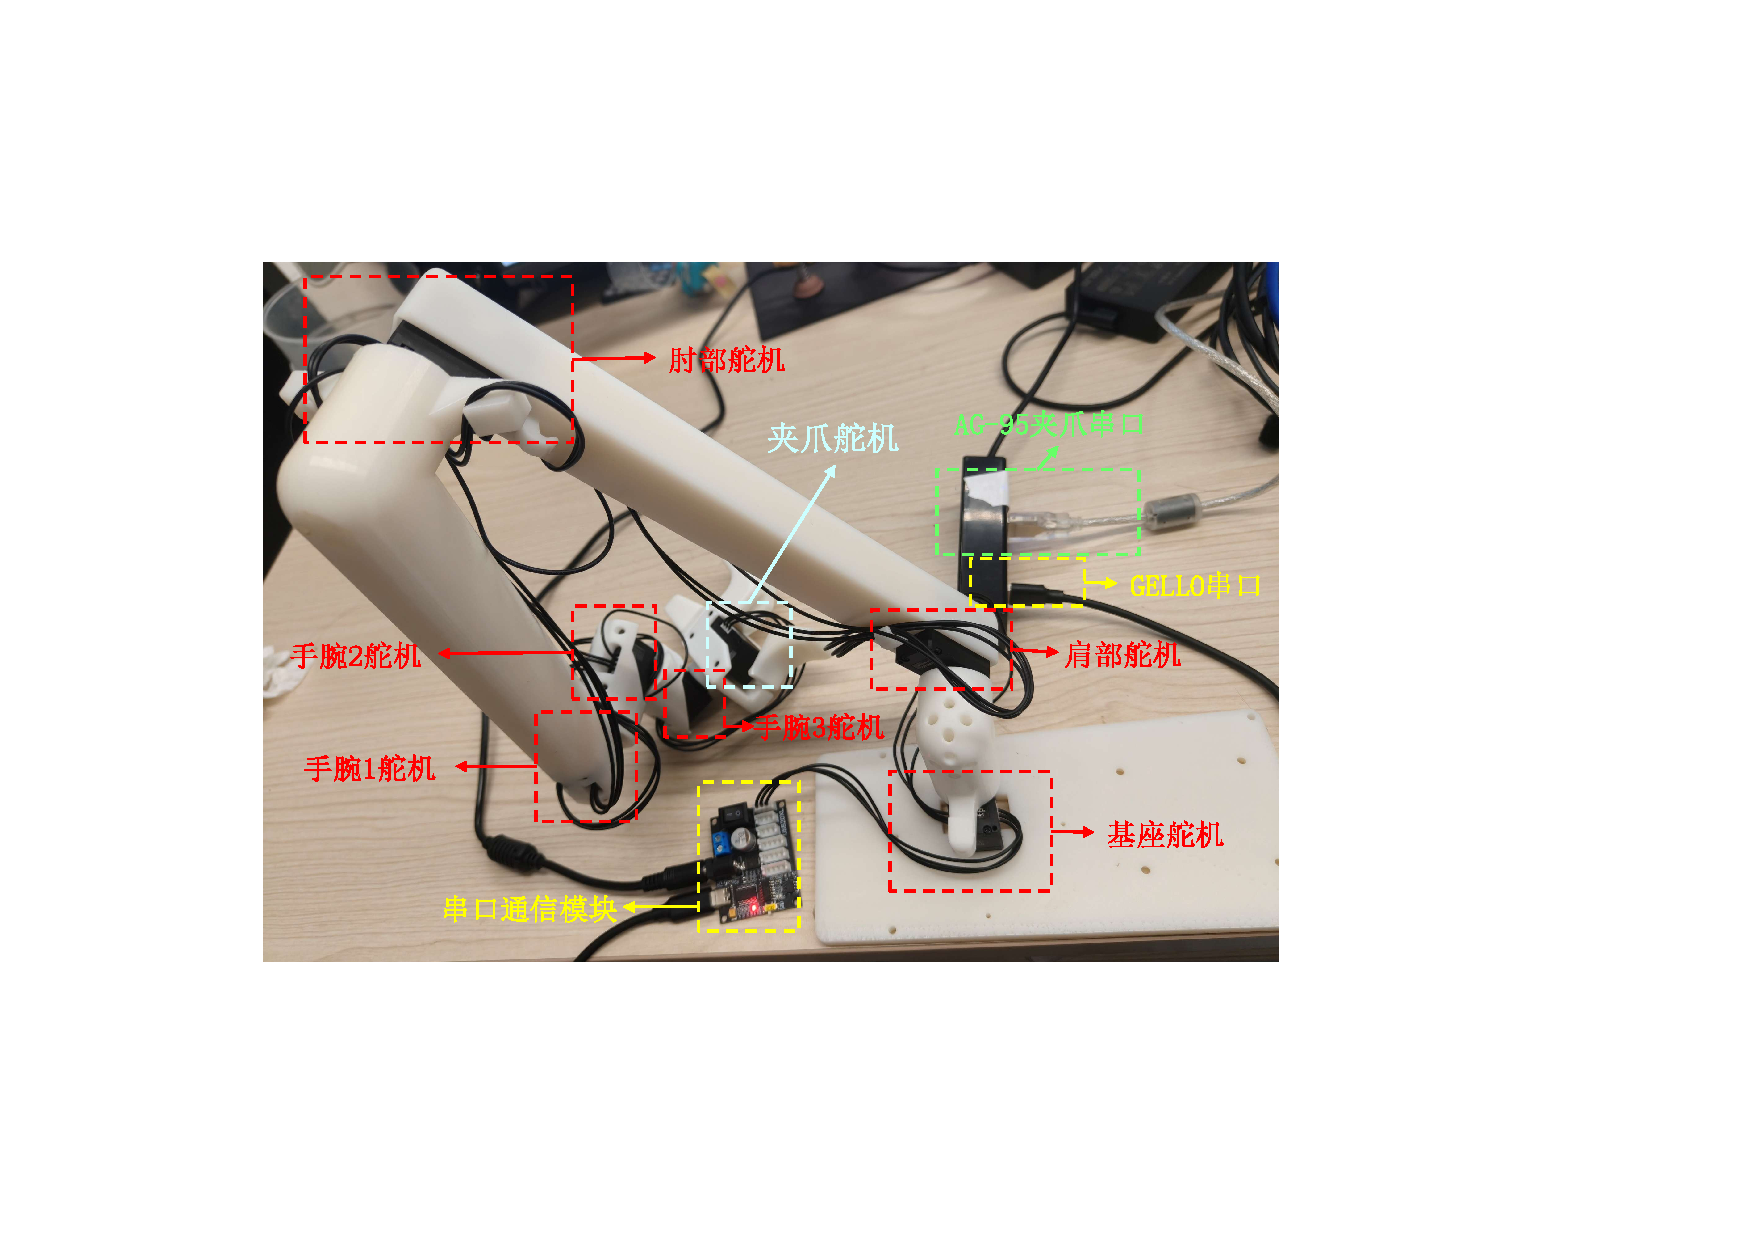
\includegraphics[width=0.8\linewidth]{figures/content/gello_pic.pdf}
  \caption{GELLO遥操臂实物图}
  \label{fig:gello_pic}
\end{figure}

在具体的关节映射关系与通信拓扑上，如图~\ref{fig:gello_pic}~所示，GELLO遥操臂的六个主干舵机与UR5e机械臂的六个旋转关节保持严格的对应关系。此外，遥操臂末端额外配置了第七个舵机，专门用于映射DH-AG95夹爪的开合状态。这七个Dynamixel舵机通过菊花链方式连接至一个串口通信模块，随后该模块的输出与夹爪的串口通信线共同接入一个USB集线器，最终统一连接至上位机PC。

\subsection{软件驱动}
\label{subsec:software_driver}

硬件平台的搭建仅为遥操作提供了物理基础，要实现操作者意图向目标机械臂的可靠传递，还需要在软件层面解决设备间的通信协议差异与物理安装引入的固有误差。

由于Dynamixel舵机的绝对编码器零点与UR5e机械臂的关节零点在物理安装时难以完全对齐，若直接将舵机读数作为控制指令，目标机械臂将产生不可预期的运动。因此，在启动遥操作之前，必须对各关节的初始偏差进行标定。标定时，操作者将遥操臂摆放至预先设定的参考位姿，系统在$-8\pi$至$8\pi$的范围内，以$\pi/2$为步长遍历搜索最优的偏差值。对于第$i$个关节，系统通过计算当前舵机读数与目标关节角之间的误差，选取使误差最小的偏差值$\Delta_i$作为该关节的标定结果。标定过程的优化目标为：
\begin{equation}
  \label{eq:offset_calibration}
  \Delta_i = \arg\min_{\Delta \in S} \left| s_i \cdot (\theta_i - \Delta) - \theta_{i}^{\text{start}} \right|
\end{equation}
其中，$S$为遍历搜索的离散偏差集合，$s_i$为该关节的旋转方向符号，$\theta_i$为当前舵机的原始读数，$\theta_{i}^{\text{start}}$为预设的参考位姿角度。这些标定参数最终被写入配置文件中，在每次启动时自动加载，从而确保遥操臂的运动指令能够准确映射至目标机械臂的关节空间。

为了实现低延迟的真机跟随运动，本平台利用了UR5e机械臂提供的实时数据交换（Real-Time Data Exchange, RTDE）接口。RTDE协议支持500 Hz的控制频率，可满足遥操作对低延迟响应的需求。在具体实现中，系统通过RTDE接口的伺服指令，将标定后的遥操臂关节角度下发至UR5e控制器。为了保证运动的平滑性与安全性，伺服指令的角速度与角加速度均被限制在0.5 rad/s及0.5 rad/s$^2$，同时设置了0.2 s的前瞻时间与100的比例增益。在该控制参数下，目标机械臂的关节跟随延迟控制在2 ms以内。

在夹爪控制方面，由于DH-AG95夹爪的控制接口接受的是0至1000的位置指令，这与其他旋转关节的弧度制指令完全不同，因此需要建立两者之间的映射关系。为了实现精确的开合控制，系统首先需要获取夹爪电机的物理边界。操作者通过手动按动遥操臂末端的夹爪电机，分别记录其在全开与全闭状态下的绝对角度值。在运行期间，系统实时读取该电机的当前角度，并根据记录的边界值将其线性归一化至0至1的区间，其中0代表完全张开，1代表完全闭合。随后，该归一化变量按下式转换为目标夹爪的位置指令：
\begin{equation}
  \label{eq:gripper_mapping}
  p_{\text{gripper}} = (1 - v_{\text{norm}}) \times 1000
\end{equation}
其中，$v_{\text{norm}}$为遥操臂夹爪舵机的归一化关节角，$p_{\text{gripper}}$为目标夹爪的位置指令。为了抑制操作者手部微小抖动对夹爪控制的干扰，系统在桥接节点中引入了滑动窗口滤波机制。该节点维护一个0.1 s的时间窗口，取窗口内指令的中位数作为当前时刻的有效输出，并设定了最小变化阈值。只有当新指令与上一有效指令的差值超过该阈值时，系统才会向夹爪发送更新命令，从而避免因手部微小抖动引发的夹爪频繁动作。

\subsection{数据采集与处理}
\label{subsec:data_collection_processing}

本平台参照LIBERO数据集的场景设置，搭建了如图~\ref{fig:real_robot_pic}~所示的机器人桌面操作场景。该场景主要划分为两个功能区域：左侧为抓取工作区，放置了多种供机器人操作的物体；右侧为抽屉操作区，放置了一个多层透明抽屉柜。在感知配置上，系统遵循LIBERO的单视角设定，在场景前方部署了一个固定视角的RGB相机，用于同时覆盖机器人本体与操作区域。

\begin{figure}[htbp]
  \centering
  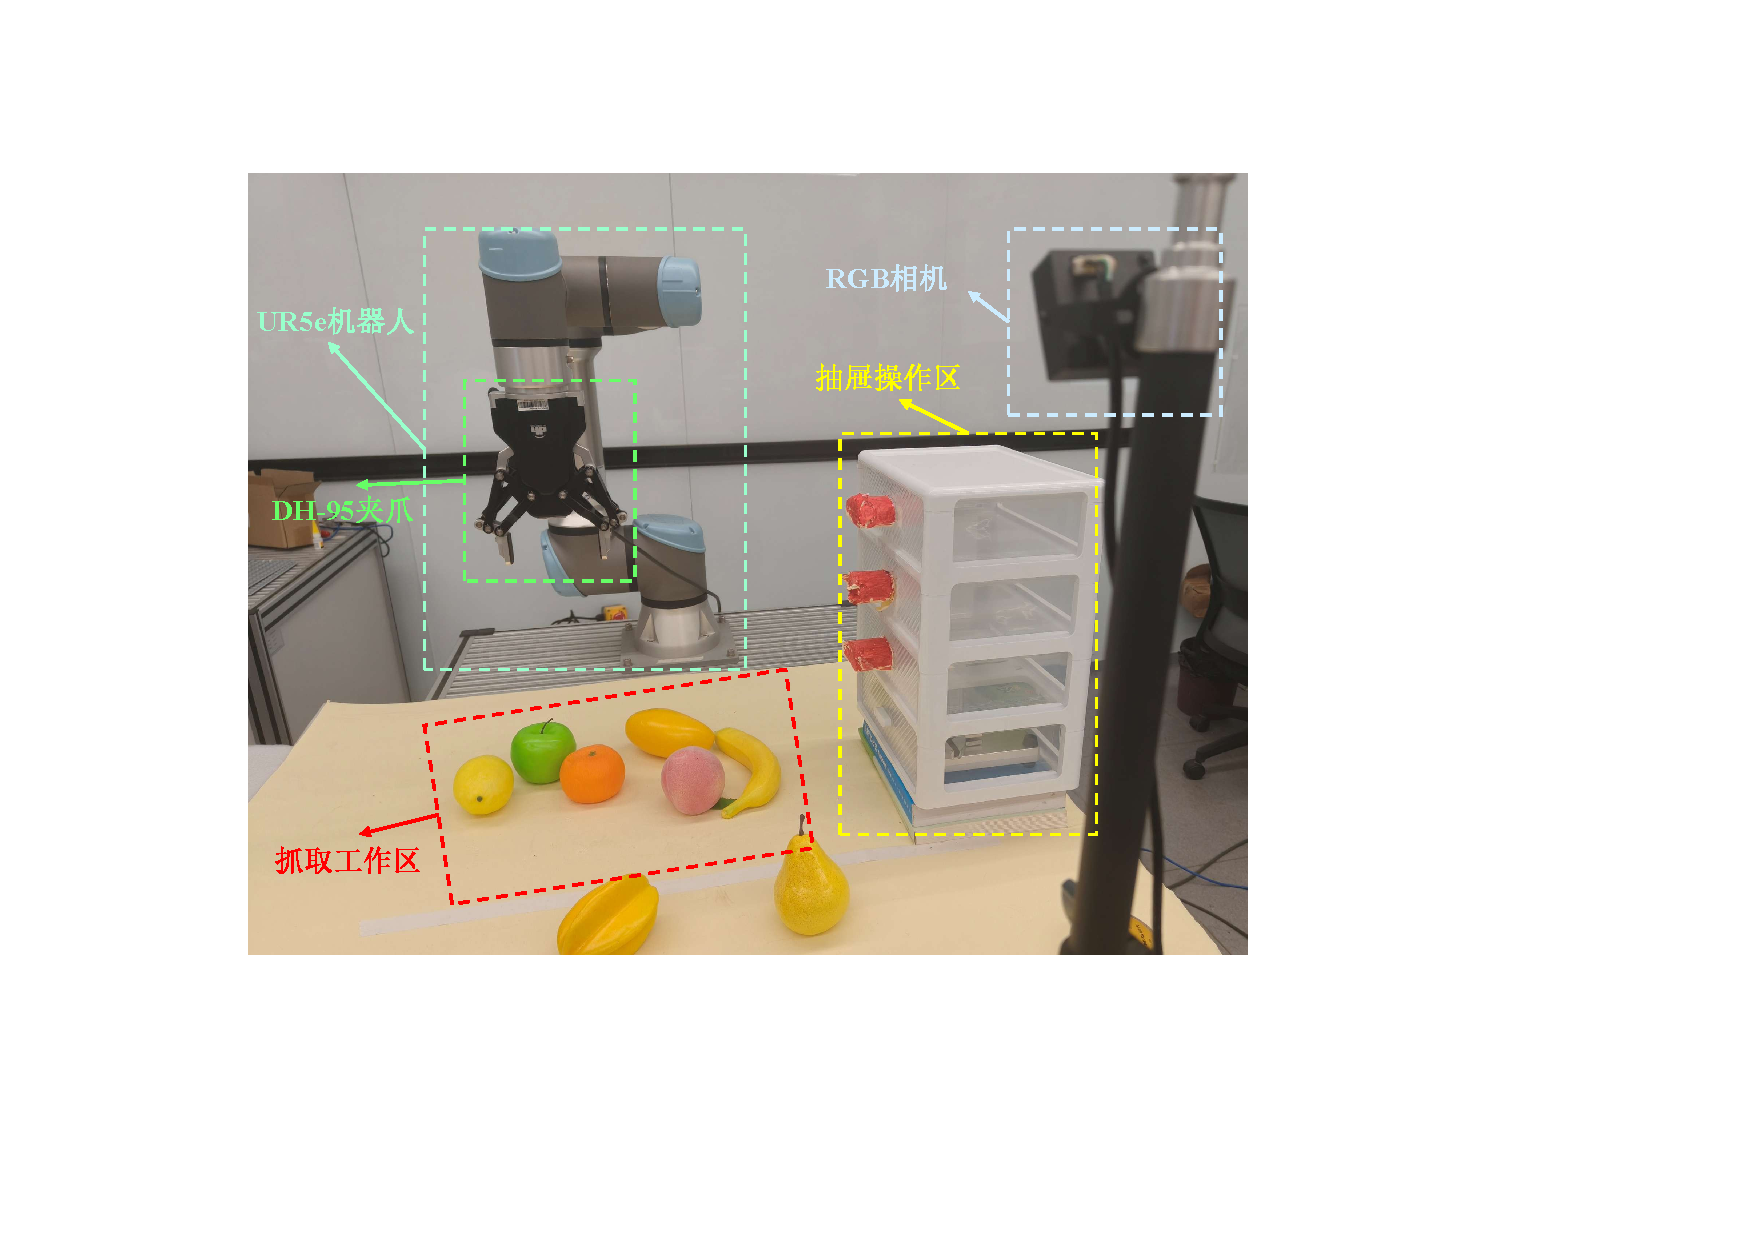
\includegraphics[width=0.8\linewidth]{figures/content/real_robot_pic.pdf}
  \caption{真实机器人桌面操作场景}
  \label{fig:real_robot_pic}
\end{figure}

基于上述场景，本章按操作复杂度设计了如表~\ref{tab:dataset_statistics}~所示的三类任务，即如图~\ref{fig:task_trajectories_placeholder}~所示的简单抓取任务、抽屉操作任务以及长时效任务，系统共引入了10种不同外观的水果模型以及2种不同高度的抽屉作为操作目标。

\begin{figure}[htbp]
  \centering
  % 占位图：采集的不同类型任务的轨迹样例
  \includegraphics[width=0.9\linewidth]{example-image-a}
  \caption{不同类型任务的采集轨迹样例}
  \label{fig:task_trajectories_placeholder}
\end{figure}

由于本章采用扩散模型作为动作生成模型，单纯依赖多样化的专家运动轨迹并不足以满足其对动作分布的学习要求。当模型在推理过程中因累积误差偏离专家轨迹时，往往难以自主调整并恢复到正确的执行路径中。为了解决这一问题，本章在常规专家轨迹之外，专门采集了200条纠错轨迹。在采集纠错轨迹时，操作者故意引导机械臂向各个错误方向运动，随后再将其纠正回正确的操作路径，从而丰富了动作分布。图~\ref{fig:correction_trajectories_placeholder}~展示了纠错轨迹的典型样例。

\begin{figure}[htbp]
  \centering
  % 占位图：纠错轨迹的样例
  \includegraphics[width=0.6\linewidth]{example-image-b}
  \caption{纠错轨迹样例}
  \label{fig:correction_trajectories_placeholder}
\end{figure}

\begin{table}[htbp]
  \centering
  \caption{真实场景数据采集任务与轨迹数量统计}
  \label{tab:dataset_statistics}
  \begin{tabular}{lp{0.5\textwidth}cc}
    \toprule
    \textbf{任务类型} & \textbf{任务描述} & \textbf{最大步数} & \textbf{轨迹数量} \\
    \midrule
    简单抓取 & 拿起[水果] & 150 & 150 \\
    抽屉操作 & 打开第[几]个抽屉 & 300 & 150 \\
    长时效任务 & 打开第[几]个抽屉并把[水果]放在里面 & 500 & 200 \\
    纠错轨迹 & -- & 600 & 200 \\
    \bottomrule
  \end{tabular}
\end{table}

如图~\ref{fig:data_collection}~所示，操作者通过观察RGB相机实时回传的图像画面，转动GELLO遥操臂来控制UR5e机械臂执行相应的操作任务。在遥操作过程中，PC控制中枢运行采集主控脚本，以30 Hz的频率同步记录相机的RGB图像帧以及机械臂当前的关节位置与夹爪状态。

\begin{figure}[htbp]
  \centering
  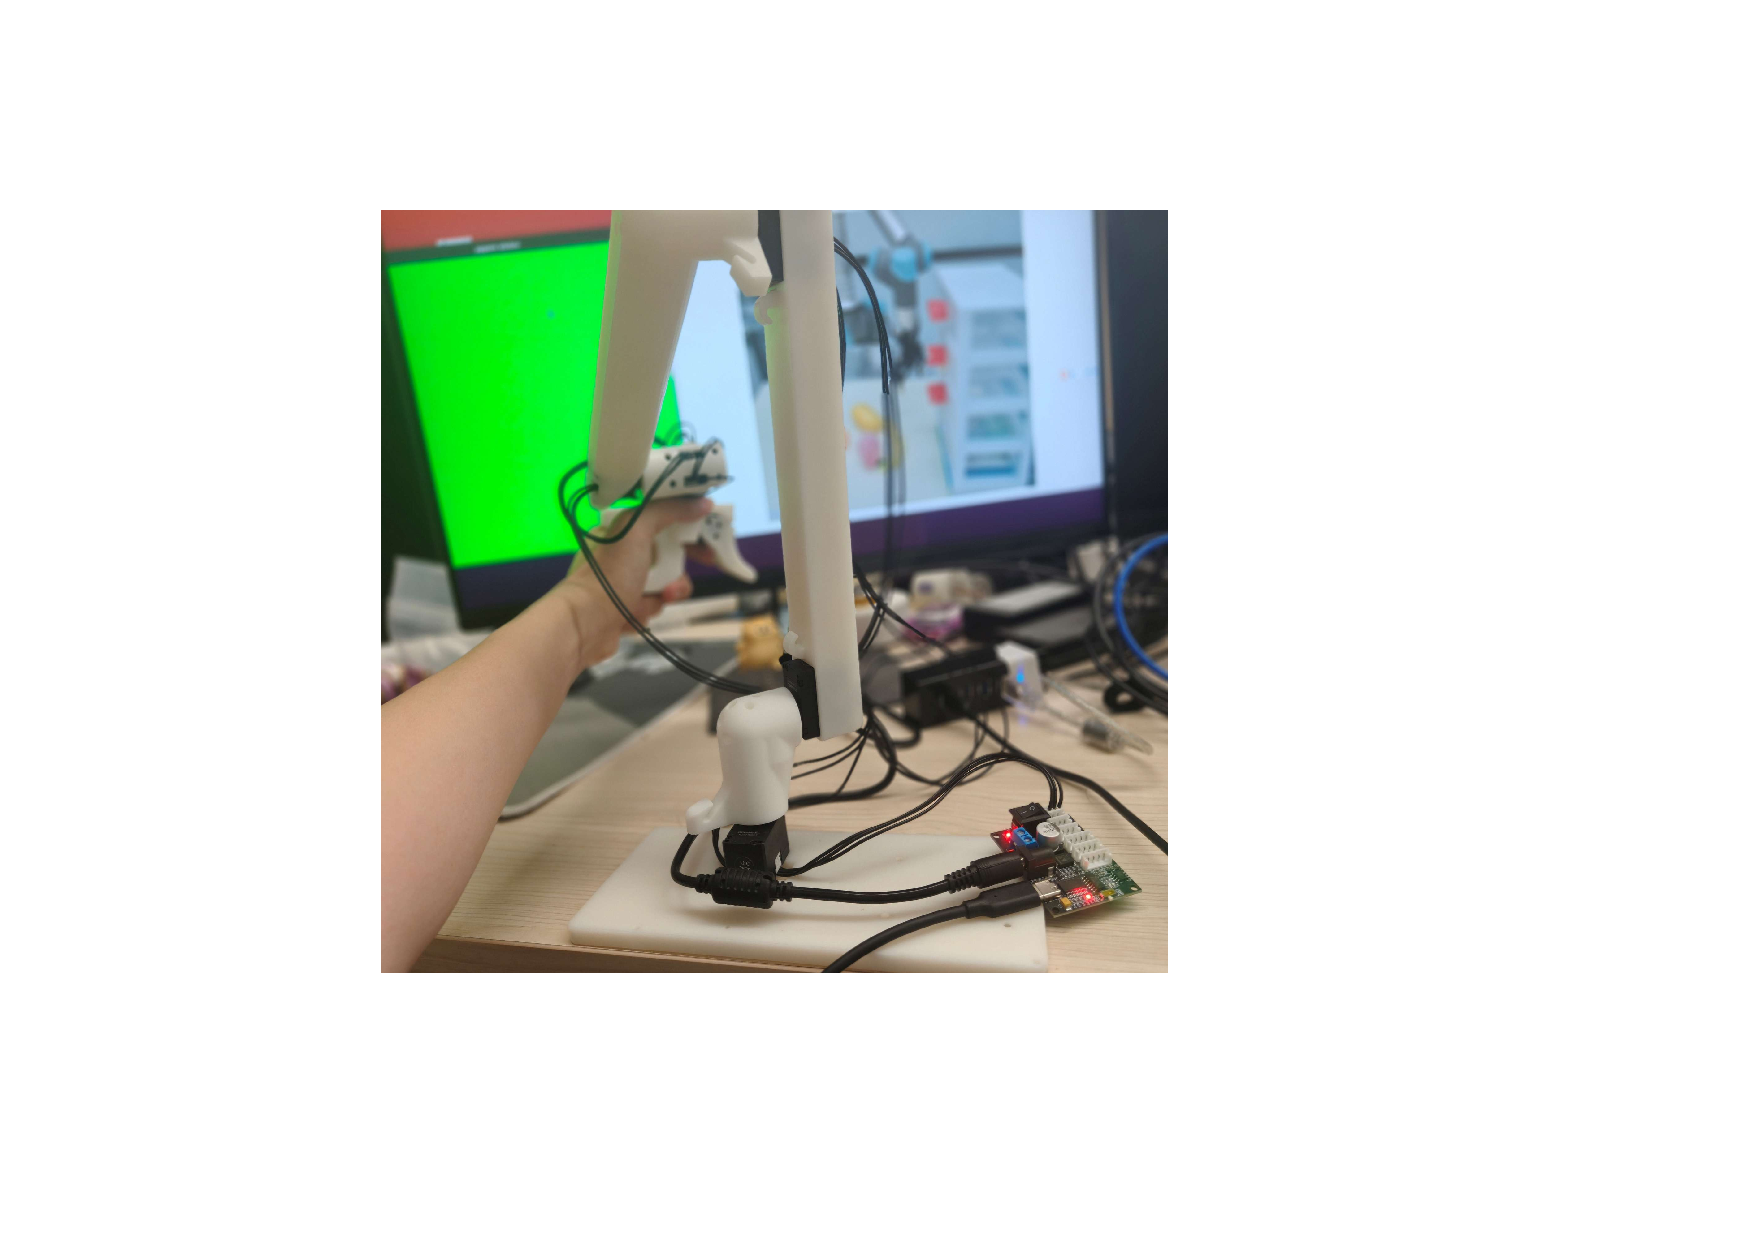
\includegraphics[width=0.6\linewidth]{figures/content/data_collection.pdf}
  \caption{基于GELLO的遥操作数据采集流程}
  \label{fig:data_collection}
\end{figure}

原始采集数据以关节角序列的形式存储，在构建训练数据集前，需要先确定动作表征的形式。在模仿学习中，动作空间的表征方式对模型的学习效果与泛化能力具有重要影响。如果直接以关节角作为学习目标，模型无需经过逆运动学求解，能够直接输出底层控制指令。然而，关节角表征对机器人的初始状态存在强依赖，在不同起始位姿下执行相同语义的任务时，关节角的输出差异往往较大，导致模型难以泛化至未见过的初始状态。相比之下，以末端执行器位姿作为学习目标，能够使模型学到的动作表征更贴近任务层面的语义逻辑，提升跨场景的泛化能力。尽管这种方式在实际控制时需要依赖逆运动学求解，且扩散模型在推理时可能偶尔生成幅度较大的动作指令，但可以通过在逆运动学求解阶段引入安全保护机制来规避风险。因此，本章采用末端位姿差分作为动作表征。

本章遵循机器人学习数据系统（RLDS，Robotics Learning Data System）的数据规范，开发了定制化的数据集构建脚本。脚本读取每帧记录的真实关节角度 $\theta_t \in \mathbb{R}^6$，利用式~\ref{eq:forward_kinematics}~的UR5e正运动学模型与DH参数，计算出末端法兰的齐次变换矩阵 $T_6^0$。由于夹爪安装在法兰末端，系统沿末端坐标系Z轴引入17 cm的工具中心点偏移。经过该偏移计算，最终得到包含夹爪末端位置 $p_t$ 与姿态旋转矩阵 $R_t$ 的完整位姿矩阵 $T_{\text{tcp}}$。

通过计算相邻两帧末端位姿的差值，系统构建出动作标签。平移差值 $\Delta p$ 直接由相邻两帧的位置向量相减得到：

\begin{equation}
  \Delta p = p_{t+1} - p_t
\end{equation}

旋转差值 $\Delta R$ 通过相邻两帧的旋转矩阵计算相对旋转，并利用对数映射 $\text{Log}(\cdot)$ 转换为三维旋转向量 $\Delta r$：

\begin{equation}
  \Delta R = R_{t+1} R_t^{-1}, \quad \Delta r = \text{Log}(\Delta R)
\end{equation}

结合夹爪的开合状态指令 $g_{t+1}$，最终构建出7维的动作标签向量 $a_t$：

\begin{equation}
  a_t = [\Delta p_x, \Delta p_y, \Delta p_z, \Delta r_x, \Delta r_y, \Delta r_z, g_{t+1}]^T
\end{equation}

构建完成的数据集在动作分布上呈现出若干值得关注的特征。不同任务对动作的要求不同，导致其平移和旋转的分布存在差异。图~\ref{fig:action_dist_task_norm}~展示了抓取任务与抽屉操作任务在平移幅值和旋转幅值上的分布对比，其中平移幅值定义为单步末端位姿平移分量的二范数，旋转幅值定义为旋转向量的二范数。抽屉操作任务的平移幅值分布尾部更长，这与其需要持续拉动抽屉的运动特性有关；而抓取任务的旋转幅值更集中在0附近，因为在接近目标物体的过程中末端姿态通常保持相对固定。

\begin{figure}[htbp]
  \centering
  \subfloat[平移幅值分布对比]{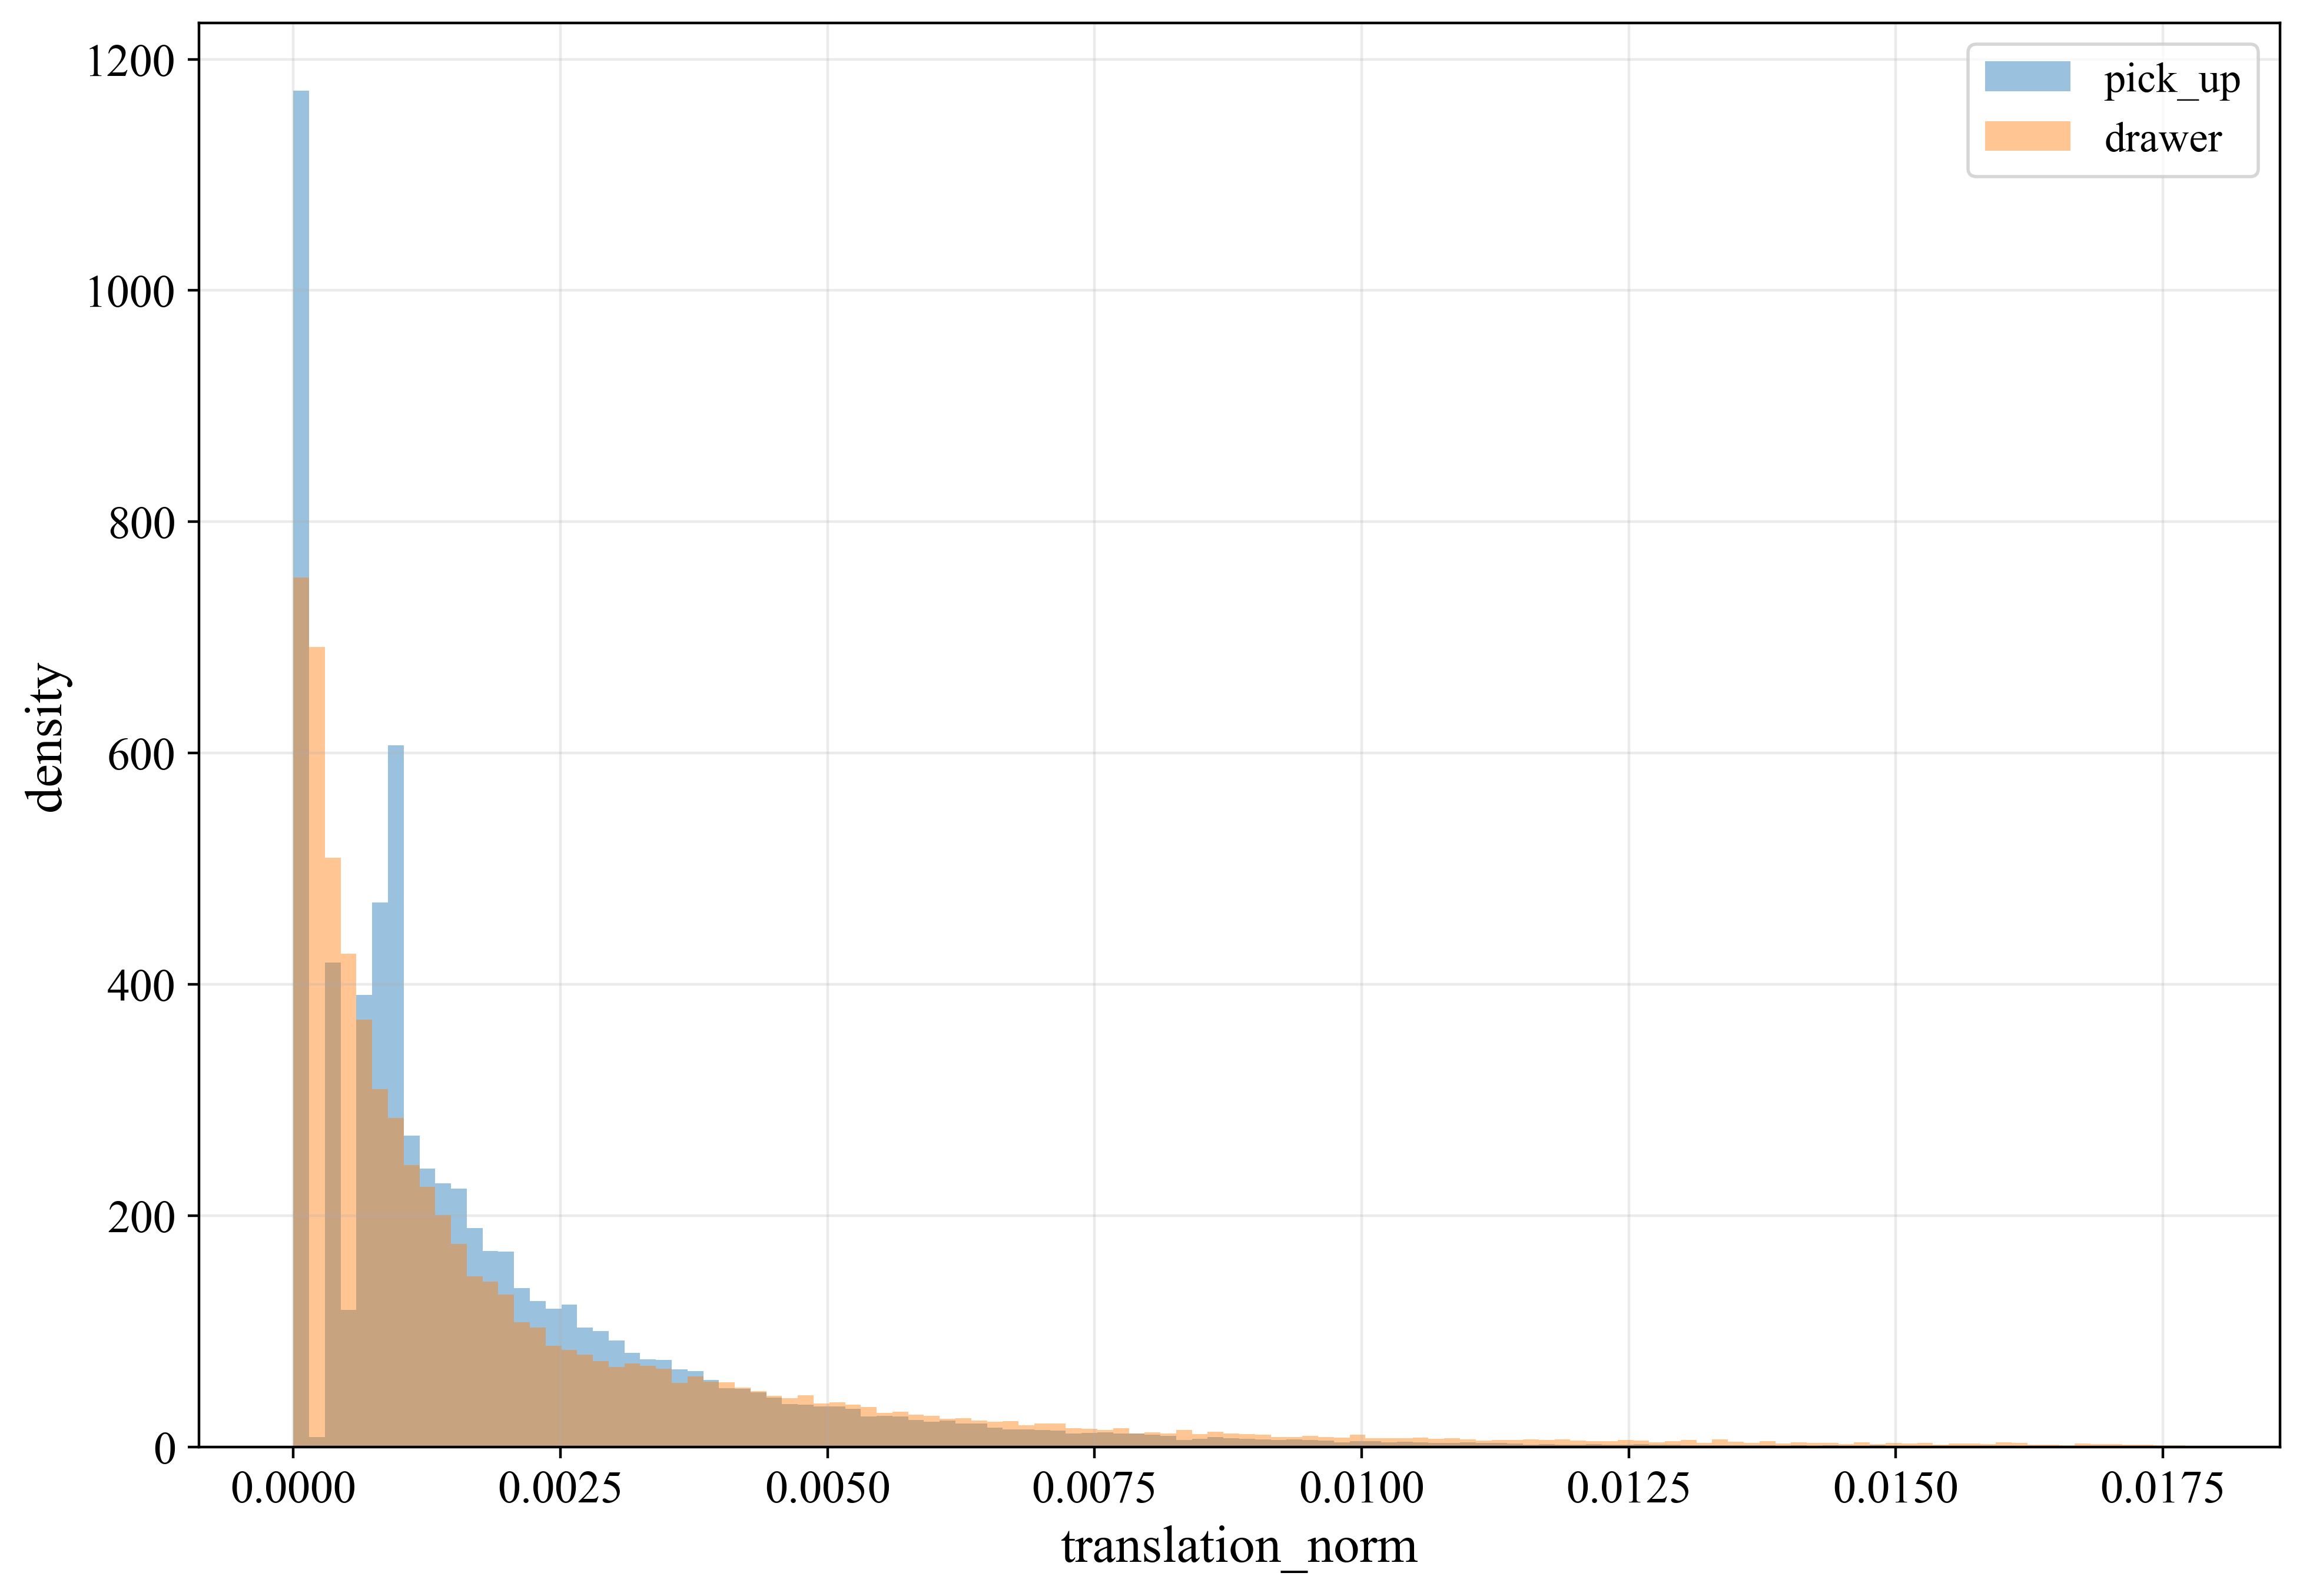
\includegraphics[width=0.48\linewidth]{figures/content/action_dist_task_trans_norm.png}\label{fig:action_dist_task_trans_norm}}
  \hfill
  \subfloat[旋转幅值分布对比]{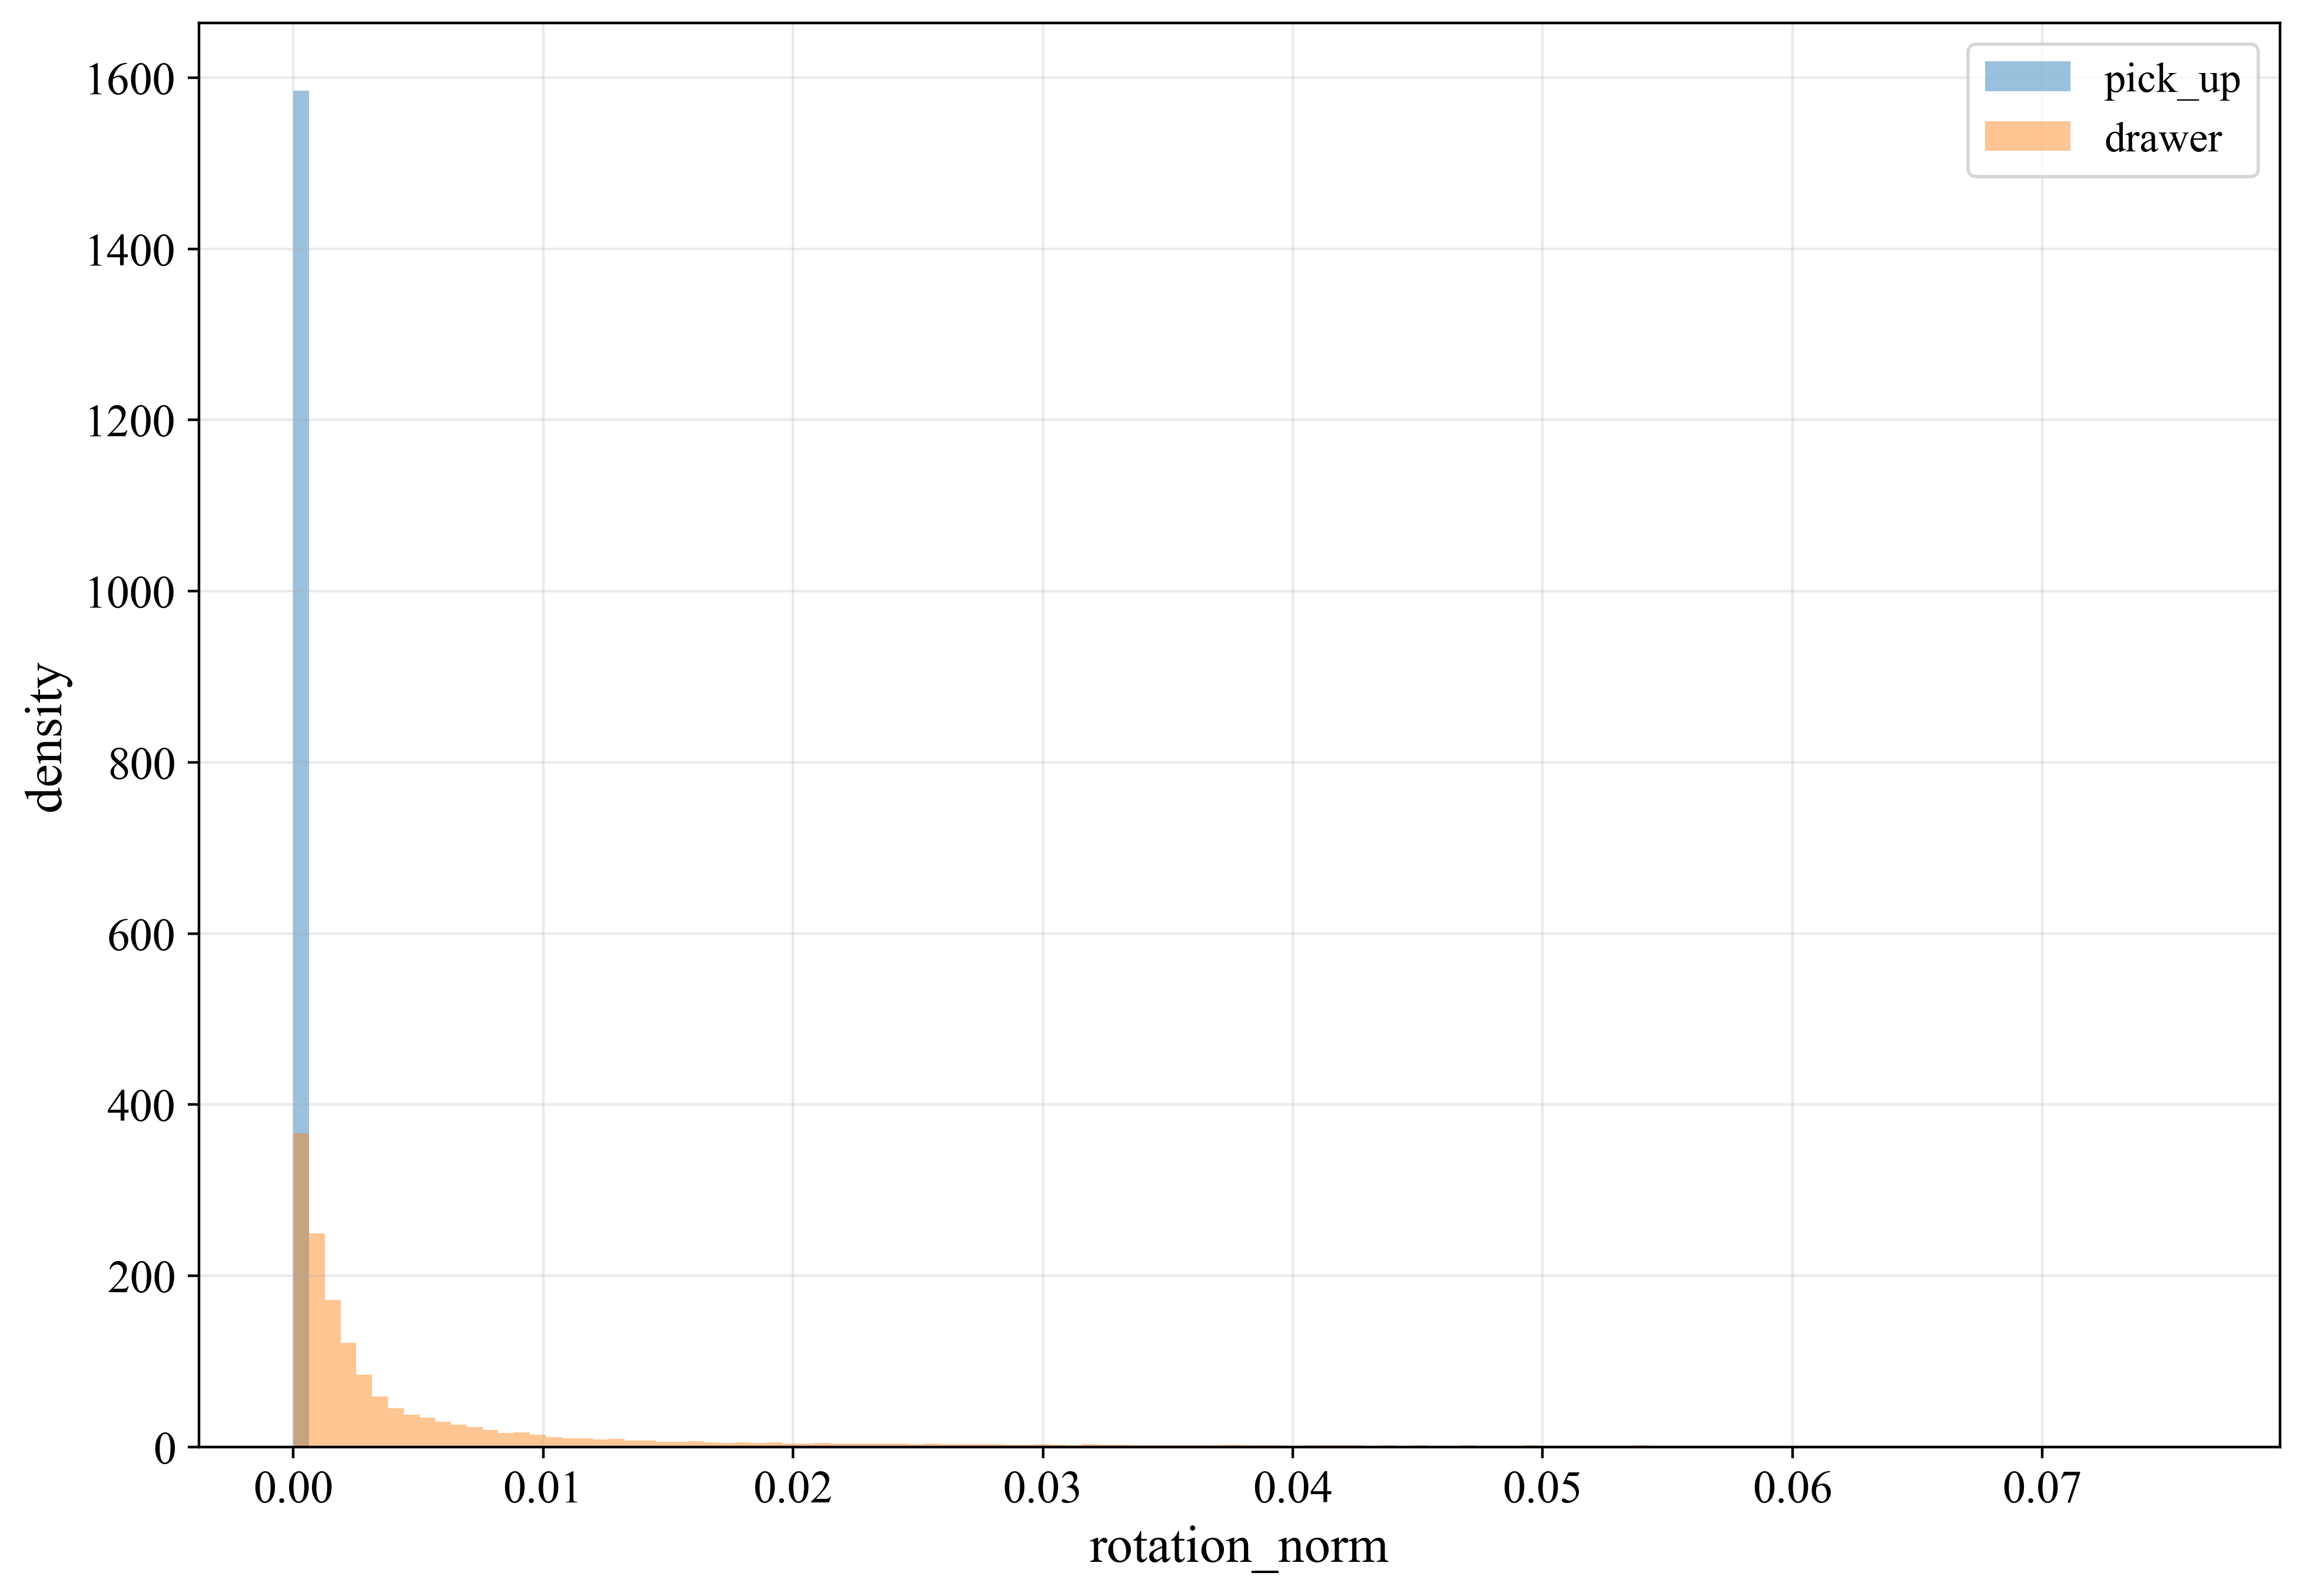
\includegraphics[width=0.48\linewidth]{figures/content/action_dist_task_rot_norm.png}\label{fig:action_dist_task_rot_norm}}
  \caption{抓取任务与抽屉操作任务动作幅值分布对比}
  \label{fig:action_dist_task_norm}
\end{figure}

除动作幅值外，各动作维度的相关性同样存在差异。图~\ref{fig:action_dist_corr}~展示了抓取任务与抽屉操作任务的动作维度相关系数热图。在抓取任务中，三个旋转分量之间呈现高度共线关系，且平移与旋转分量之间的相关系数接近0，说明该任务的平移与旋转相对解耦。而在抽屉操作任务中，沿 $x$ 轴的平移与绕 $y$ 轴的旋转存在中等程度的负相关，反映了操作者在拉动抽屉时手臂前伸与腕部俯仰的协调配合。两类任务在动作维度耦合结构上的差异，决定了各自策略的学习难点不同。

\begin{figure}[htbp]
  \centering
  \subfloat[抓取任务动作维度相关性]{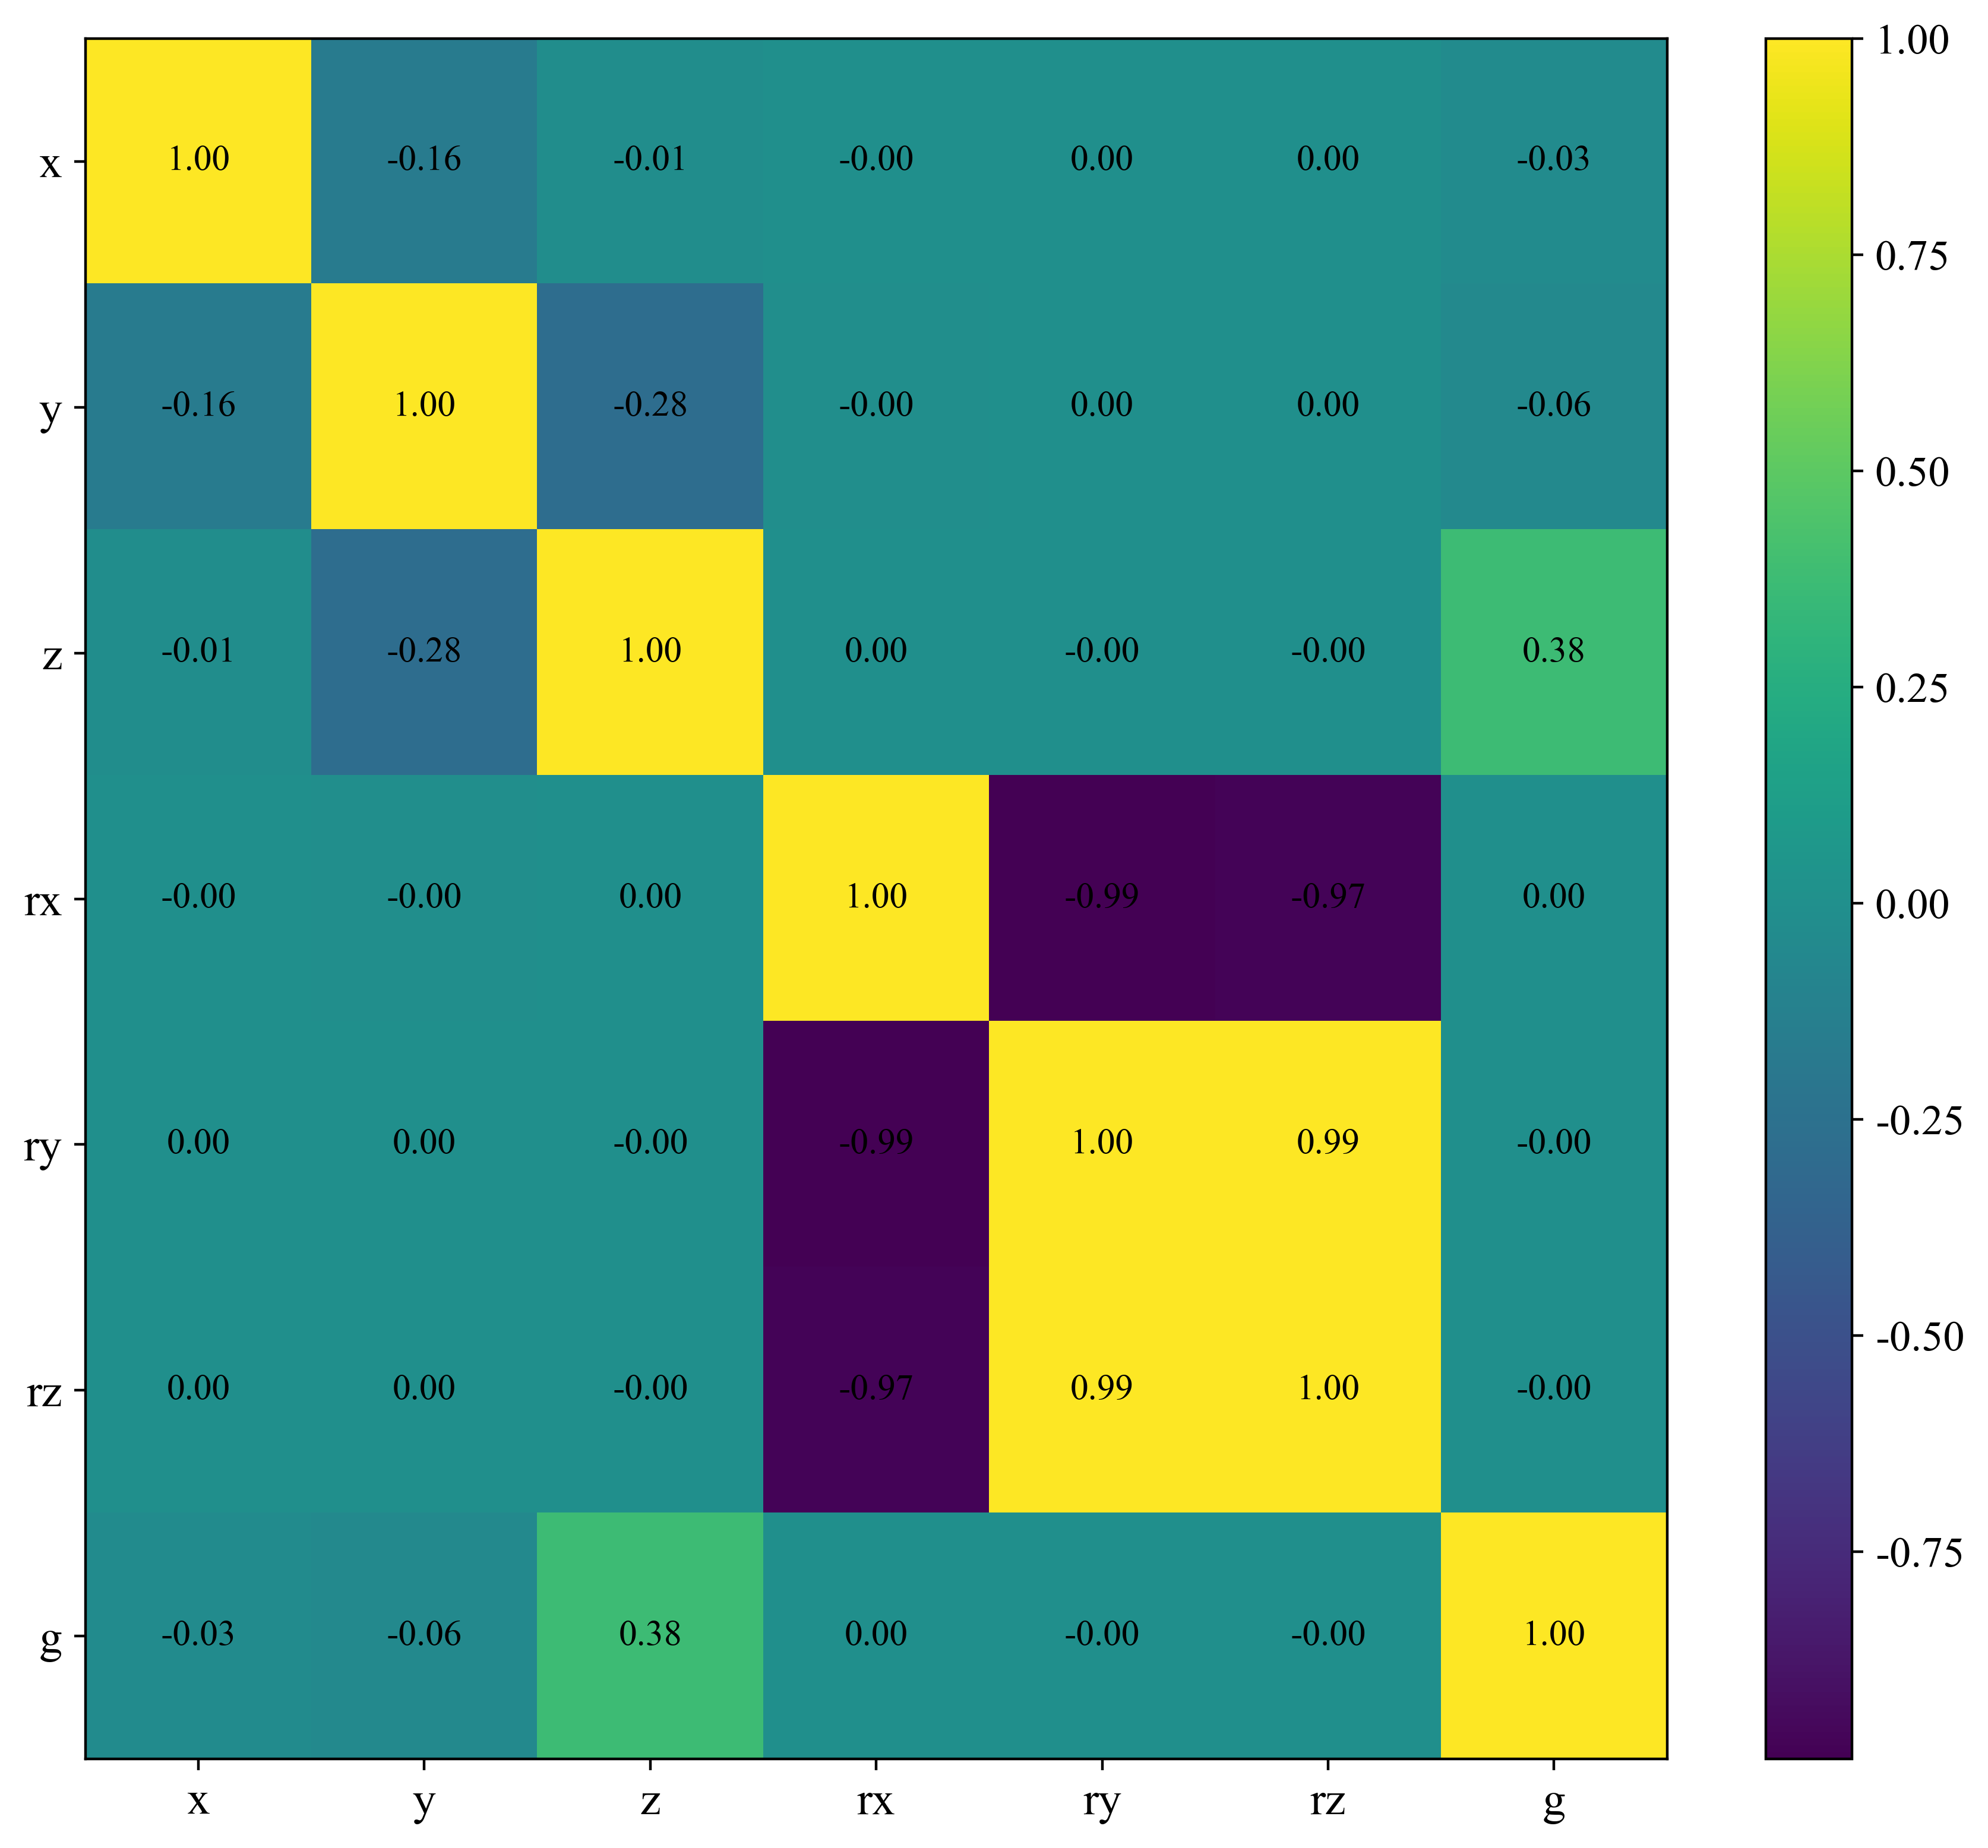
\includegraphics[width=0.48\linewidth]{figures/content/action_dist_corr_pickup.png}}
  \hfill
  \subfloat[抽屉操作任务动作维度相关性]{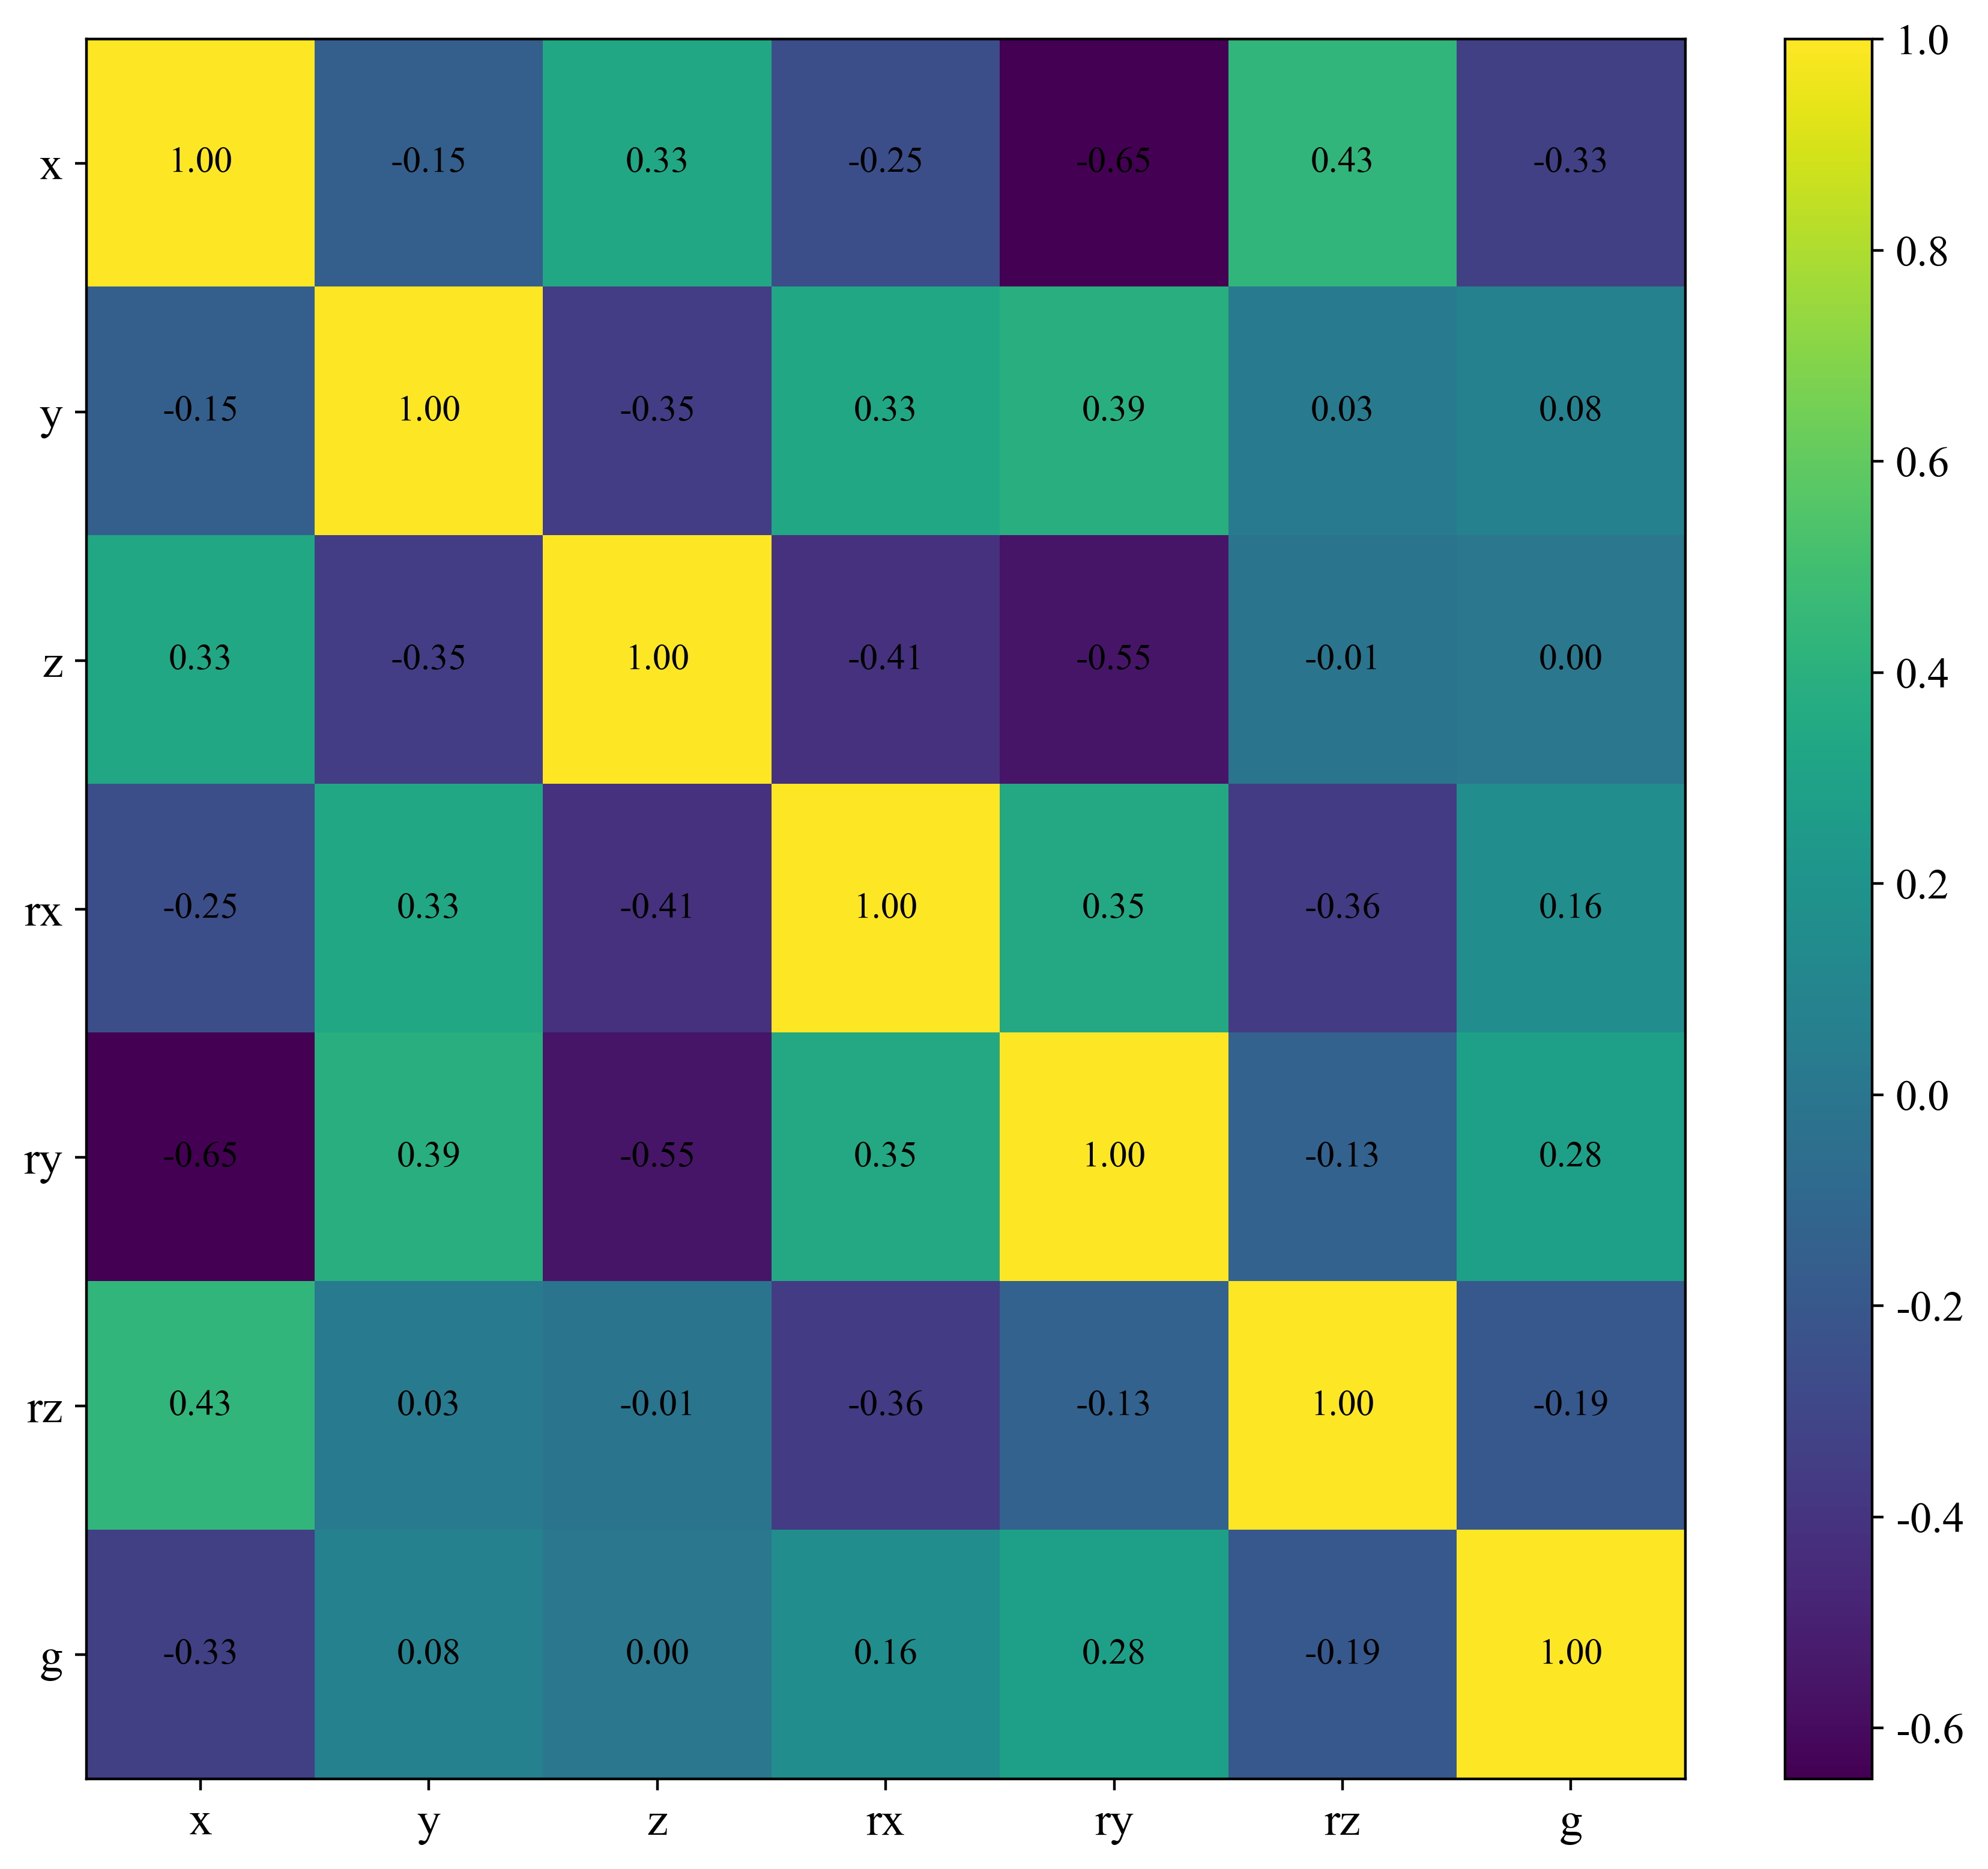
\includegraphics[width=0.48\linewidth]{figures/content/action_dist_corr_drawer.png}}
  \caption{不同任务类型动作维度相关性对比}
  \label{fig:action_dist_corr}
\end{figure}

真实场景采集的数据与仿真环境数据在动作分布上同样存在差异。图~\ref{fig:action_dist_long_vs_libero}~展示了自建长时效任务数据集与LIBERO仿真数据集在平移和旋转幅值上的分布对比。在采集真实数据时，出于对机器人的安全保护，操作者倾向于以较小的步幅控制机械臂运动，因此真实数据的平移与旋转幅値分布在0附近更为密集。LIBERO仿真环境无需这一层安全考量，仿真模型可以按照任务要求执行较大幅度的动作。

\begin{figure}[htbp]
  \centering
  \subfloat[平移幅值分布对比]{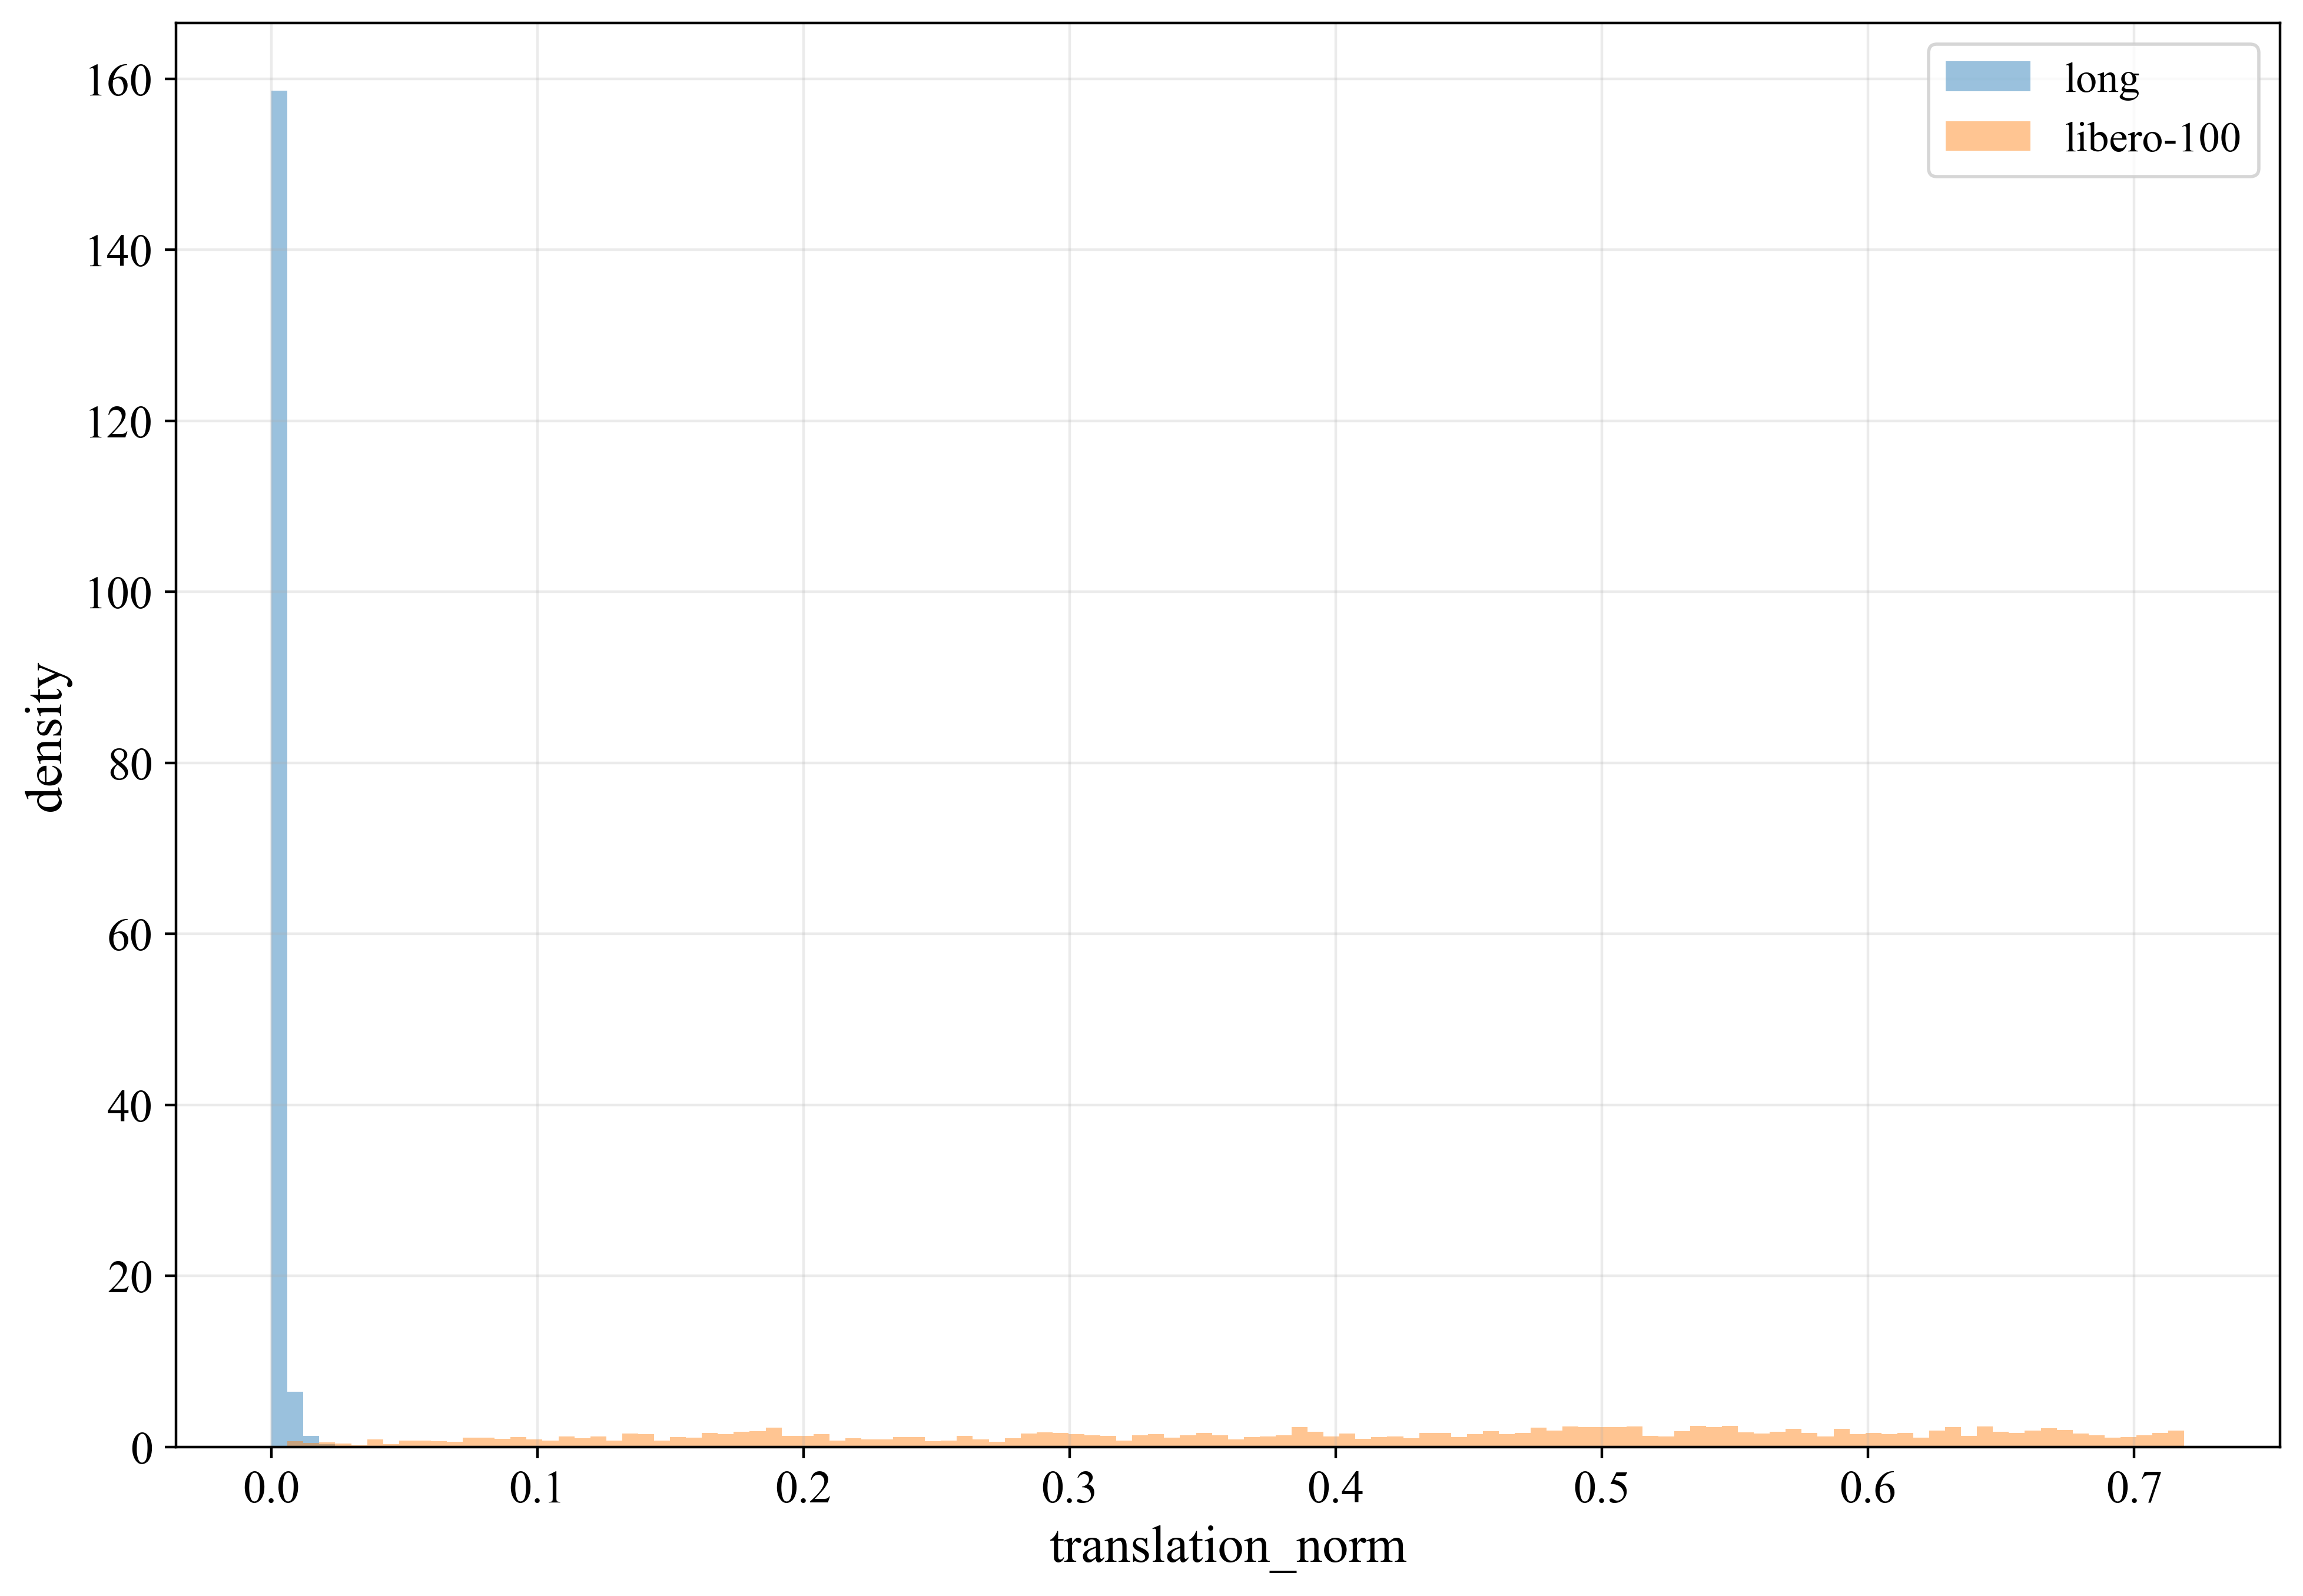
\includegraphics[width=0.48\linewidth]{figures/content/action_dist_long_vs_libero_trans.png}\label{fig:action_dist_long_vs_libero_trans}}
  \hfill
  \subfloat[旋转幅值分布对比]{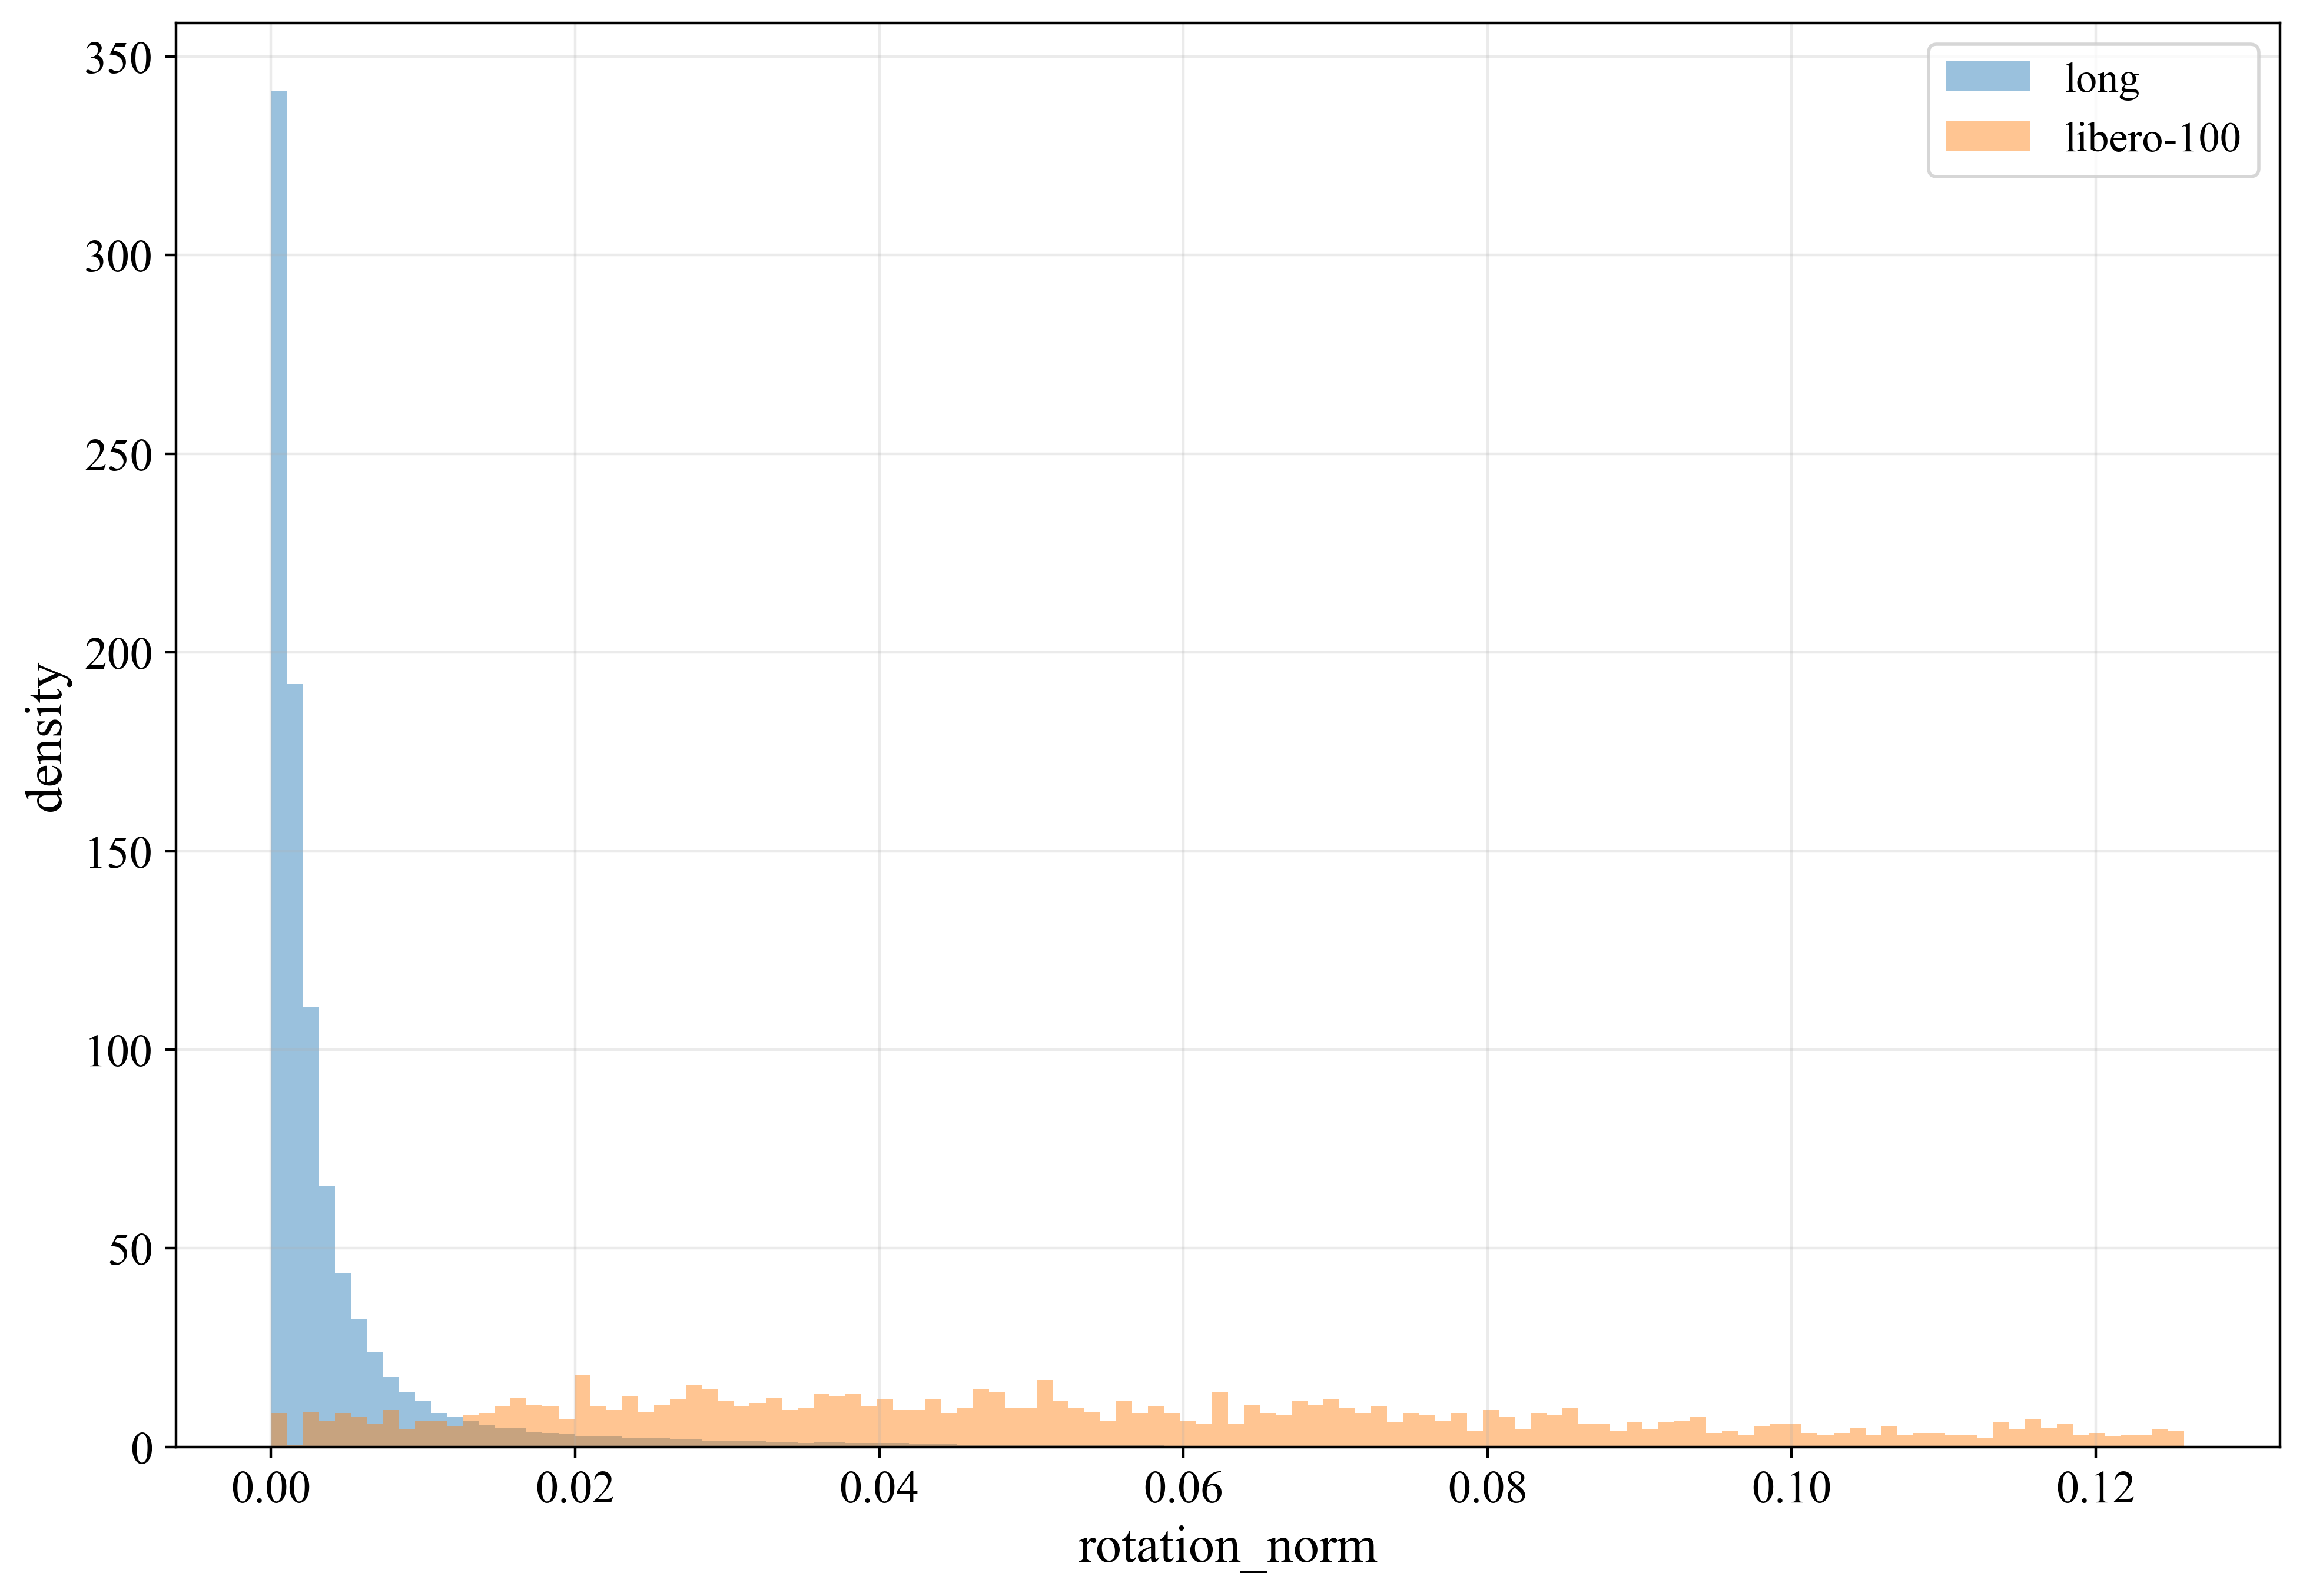
\includegraphics[width=0.48\linewidth]{figures/content/action_dist_long_vs_libero_rot.png}\label{fig:action_dist_long_vs_libero_rot}}
  \caption{长时效任务真实场景与仿真环境动作幅值分布对比}
  \label{fig:action_dist_long_vs_libero}
\end{figure}

\section{基于ROS的机械臂在线推理与控制系统}
\label{sec:ros_inference_control_system}

在完成5.1节所述的真实场景数据采集与处理后，系统获得了可供训练的机器人动作数据集。有了这些数据，便可以对视觉语言动作模型进行微调训练，使其适应真实环境。然而，由于大参数量模型难以直接在边缘计算设备上进行部署，为了满足机器人控制的实时性要求，本节设计了计算与控制分离的架构，搭建了模型推理的远端服务。在此基础上，结合ROS开发了机械臂动作控制系统，将远端推理出的动作序列安全、稳定地转化为底层控制信号，最终实现从感知到执行的完整闭环。

\subsection{视觉语言动作模型的微调与远端服务部署}
\label{subsec:model_finetuning_deployment}

如前文5.1节所述，真实场景采集到的遥操作动作与LIBERO等仿真环境的动作在分布上存在显著差异。真实操作往往伴随着更小的动作幅值、更频繁的微调以及更复杂的物理约束，这导致预训练模型在仿真数据上学到的动作分布难以直接迁移。如果直接采用仿真预训练时的超参数设定进行微调，模型在真实数据上的训练损失会出现剧烈波动，难以收敛到稳定的局部最优解。

为了解决这一问题，本节经过大量实验尝试，最终确定了一组能够保证训练稳定收敛且波动较小的微调超参数。具体而言，模型的基础学习率设定为 $2 \times 10^{-6}$，这一较低的学习率可以防止在真实数据微调初期破坏预训练阶段建立的特征表示；学习率调度策略采用线性预热结合余弦衰减（linear-warmup+cosine-decay），其中预热比例设为0.02，使得模型在训练前期的梯度更新更加平缓；同时，最大梯度裁剪范数设定为0.5，权重衰减系数设为0.001，以进一步抑制梯度爆炸现象并防止过拟合。在上述配置下，模型在真实数据集上训练4000步后即可达到稳定状态，完成从仿真动作分布向真实操作动作分布的适配。

微调完成后，模型需要被部署为可供控制端调用的在线推理服务。考虑到视觉语言动作模型本身参数量大，其初始化过程涉及大量权重加载与显存分配，若每次推理时重新加载模型将导致不可接受的延迟。因此，系统必须在远端服务器上将模型常驻于显存中运行，通过HTTP协议持续监听并响应来自控制端的请求，以此保证推理的实时性。

在动作生成的具体配置上，结合真实采集数据的特性，系统对推理阶段的超参数进行了调整。如前文所述，在遥操作采集数据时，出于安全考虑，操作者给定的动作步幅通常较小，这使得单步动作在空间上的位移十分有限。为了保证机械臂在执行时动作能够更快地连贯进行，本节将模型推理的动作分块（Action Chunking）长度设置为15步。也就是说，单次推理请求将一次性返回未来15个时间步的预测动作。与动作分块相对应，由于真实场景下任务耗时更长、步幅更小，模型需要记忆更长的时间跨度才能维持有效的历史上下文，因此在真机实验中，将时序缓存机制的存储长度扩展设定为256帧。

在常驻服务器运行的推理服务中，为了防止由于网络延迟或分块执行时间过长导致的图像与状态错位，系统引入了会话校验（Session）机制。控制端在每次发起推理请求时，会同步发送当前的会话标识符与时间戳。远端服务接收到请求后，会首先核对会话状态，确保当前传入的RGB图像观测、语言指令与缓存池中保存的历史状态在时序上严格对应。这一校验机制有效避免了长时效任务执行中可能出现的动作与视觉特征不匹配问题，进一步保障了真机操作的可靠性。

\subsection{基于ROS的机械臂动作控制系统}
\label{subsec:ros_arm_control_system}

远端推理服务搭建完成后，需要开发本地的控制中枢来桥接模型输出与硬件执行器。本节基于ROS开发了机械臂动作控制系统，通过多个节点的话题（Topic）发布与订阅机制，实现从图像采集、推理请求到逆运动学求解及底层信号下发的完整回路。

系统的核心控制节点首先通过订阅相机的图像话题获取当前工作空间的视觉状态，并结合预设的语言指令，通过HTTP请求向远端服务器发起推理。由于反归一化处理已经在推理服务内部完成，模型返回的动作序列直接就是物理尺度下的末端位姿差分与夹爪状态。控制节点在接收到这15步动作分块后，需要将其逐一转化为机械臂各关节的目标角度。为此，系统订阅了 \texttt{/joint\_states} 话题以实时获取当前机械臂的真实关节位置，并调用正运动学模型计算出当前的末端齐次变换矩阵。将模型返回的位姿差分叠加到当前位姿上后，便得到了下一时间步的目标末端位姿。随后，系统调用 trac\_ik 逆运动学求解器，计算出能够到达该目标位姿的关节角度序列。

在将计算出的关节角度下发给底层控制器之前，系统必须进行严格的安全限制。由于模型在长时效推理中可能偶尔生成幅度过大或方向突变的错误动作，如果直接执行，极易导致机械臂与桌面发生剧烈碰撞。因此，控制节点在求解前后设置了多层约束：在更新目标末端位姿时，限制单步的平移差值不超过0.03 m，旋转角度不超过0.15 rad；在逆运动学求解得到目标关节角后，系统会检查其与当前真实关节角的差值，若任一关节的跳变超过0.5 rad，或者逆运动学无解，则直接丢弃该步动作并保持机械臂原地不动。

通过上述安全校验后，系统将合法的关节角度序列打包为轨迹点，并通过 \texttt{/scaled\_pos\_joint\_traj\_controller/follow\_joint\_trajectory} 这一 Action 接口发送给UR5e的底层控制器执行。同时，夹爪的开合指令则通过单独的 \texttt{/gripper/ctrl} 话题同步发布。底层控制器在接收到轨迹后驱动伺服电机运动，并将执行后的真实关节状态再次发布到 \texttt{/joint\_states} 话题，形成闭环。这一过程在15步动作分块执行完毕后循环触发，从而实现了稳定可靠的连续动作控制。

\subsection{对比实验}
\label{subsec:real_world_experiments}

为了验证本文提出的TemporalCacheVLA模型在真实场景下的有效性，本节在UR5e真机平台上开展了对比实验。实验采用前文5.1节建立的自建数据集进行微调训练，并在与数据采集时完全相同的物理场景下进行测试验证。作为对比基线，本节选取了目前在真实机器人操作中广泛使用的OpenVLA模型。实验场景划分为简单抓取、抽屉操作以及长时效任务三类，每类任务各测试20次，记录其成功率。

在对比成功率之前，图~\ref{fig:real_trajectory_success}~首先展示了TemporalCacheVLA模型在三类任务中的成功执行轨迹。可以看出，在简单抓取任务中，机械臂能够平稳地将夹爪移动至目标水果上方并完成闭合；在抽屉操作任务中，模型学会了如何抓住抽屉把手并向后拉出足够的空间；而在长时效任务中，机械臂在关闭顶层抽屉后，能够顺利切换到抓取黑色碗的动作并将其放入底层抽屉，整个过程没有出现明显的停顿或轨迹偏移。

\begin{figure}[htbp]
\centering
\includegraphics[width=0.9\linewidth]{figures/content/real_trajectory_success_placeholder.png}
\caption{TemporalCacheVLA在三类真实任务中的成功执行轨迹}
\label{fig:real_trajectory_success}
\end{figure}

两者的成功率对比结果如表~\ref{tab:real_world_results}~所示。

\begin{table}[htb]
\centering
\caption{真实机器人平台对比实验成功率}
\label{tab:real_world_results}
\begin{tabular}{c|ccc|c}
\toprule
方法 & 简单抓取 (\%) & 抽屉操作 (\%) & 长时效任务 (\%) & 平均成功率 (\%) \\
\midrule
OpenVLA & 75 & 45 & 15 & 45.0 \\
TemporalCacheVLA & 85 & 75 & 60 & 73.3 \\
\bottomrule
\end{tabular}
\end{table}

由表~\ref{tab:real_world_results}~的数据可以看出，两者的真机实验成功率相比于第四章在LIBERO仿真环境中的表现（通常在80\%以上）均有明显下降。这是因为真实环境中的光照变化、相机视角的微小偏移以及机械臂的运动学误差，都会对基于视觉的端到端策略造成干扰。尽管如此，TemporalCacheVLA在各类任务中依然表现出了优于OpenVLA的性能。在简单抓取任务中，两者的成功率差距相对较小（85对75）；但在包含多个阶段的长时效任务中，TemporalCacheVLA的成功率达到了60，而OpenVLA仅为15。

为了深入分析长时效任务中成功率差异的原因，图~\ref{fig:real_trajectory_failure}~展示了OpenVLA在执行该任务时的典型失败案例。

\begin{figure}[htbp]
\centering
\includegraphics[width=0.8\linewidth]{figures/content/real_trajectory_failure_placeholder.png}
\caption{OpenVLA在长时效任务中的典型失败案例}
\label{fig:real_trajectory_failure}
\end{figure}

从图~\ref{fig:real_trajectory_failure}~中可以观察到，OpenVLA在完成第一个子任务（关闭抽屉）后，由于缺乏对历史上下文的记忆，模型在后续动作生成时发生了状态混淆。在抓取黑色碗的阶段，夹爪并未准确移动至碗的上方，而是在抽屉附近徘徊，最终导致任务超时失败。相比之下，本文提出的模型通过时序缓存机制，能够在执行长时效任务时保持对全局目标的关注，从而在真实物理环境中也取得了更为稳定的操作表现。

\chapter{总结与展望}
\label{chp:conclusion}

\section{研究总结}
\label{sec:conclusion}

随着人工智能与机器人技术的不断发展，具身智能作为连接数字世界与物理世界的桥梁，正成为科技发展的重点领域。然而，真实世界中的非结构化环境往往伴随着光照变化、物体层叠遮挡等复杂因素，同时长时序任务中还存在明显的历史上下文依赖，这些问题共同影响了机械臂在复杂操作任务中的成功率与可靠性。针对长时序、非结构化任务中的多模态动作生成与决策依赖难题，本文提出了一种基于特征时序缓存的视觉语言动作模型 TemporalCacheVLA。通过在仿真数据集与真实机械臂平台上的实验评估，结果表明，本文所提出的方法在多阶段、长时序操作任务中具有较好的性能表现，并在一定程度上验证了其真实部署潜力。本文的主要研究工作与结论如下：

（1）研究了基于运动学理论与典型模仿学习算法的机器人操作基础理论。针对机械臂在笛卡尔空间与关节空间之间的运动映射问题，本文基于 Denavit-Hartenberg 参数法对 Franka Panda 与 UR5e 两款机械臂进行了运动学建模。该模型推导了正向与逆向运动学方程，明确了各关节角度与末端空间位姿之间的映射关系，为后续真实场景数据集构建中的动作标签计算提供了正运动学支撑，同时也为真实部署阶段末端增量动作到关节空间控制目标的转换提供了理论基础。

（2）研究了基于扩散模型的模仿学习动作生成算法。针对传统行为克隆方法难以有效拟合多模态动作分布的问题，提出了一种结合多模态特征编码与扩散去噪的动作生成算法。该方法采用迭代 DiT 为核心架构，利用 EfficientViT 提取轻量化多尺度视觉特征。为了实现多模态特征的有效融合，设计了非对称跨模态注意力机制，在保留状态残差的同时引导多步去噪过程，并采用 DDIM 策略加速采样。实验结果表明，在 RoboMimic 数据集上，该算法在多项任务中取得了较好的性能表现。相比于基线模型，本文方法在 Transport ph 任务上取得了 $0.862$ 的成功率，在 Tool Hang ph 任务上达到 $0.791$；此外，在 Transport mh 数据集上的对比实验中，本文方法的成功率由 Diffusion Policy 的 $0.643$ 提高至 $0.801$。这些结果说明，所建立的扩散动作生成模型能够较有效地建模复杂多模态动作分布，并在生成质量与推理效率之间取得较好的平衡。

（3）研究了基于特征时序缓存的视觉语言动作模型 TemporalCacheVLA。针对机器人在长时序任务中因单帧决策导致的状态混淆与上下文遗忘问题，本文提出了一种双通道特征时序缓存机制，并在此基础上构建了 TemporalCacheVLA 模型。该模型通过感知语义双通道历史存储池分别维护历史感知信息与历史语义信息，并结合缓存检索、可学习门控融合以及基于余弦相似度的压缩更新策略，实现了对长时序上下文的高效维护与动态利用。在具体实现上，模型采用双分支视觉编码器与大语言模型进行多模态特征提取，并将增强后的上下文特征输入扩散动作生成模块。实验结果表明，在 LIBERO 基准数据集上，本文方法在强调指令跟随的 Goal 子集与包含长时序任务的 LIBERO-100 子集上分别取得了 $0.959$ 和 $0.949$ 的平均成功率。同时，在 LIBERO-100 子集上的消融实验中，移除缓存检索、门控融合与缓存压缩机制后，成功率分别下降至 $0.862$、$0.835$ 和 $0.823$。这些结果说明，双通道特征时序缓存机制能够较有效地维护和利用历史上下文信息，从而缓解长时序任务中的决策波动问题。

（4）研究了基于真实物理平台的系统部署与实验验证。针对视觉语言动作模型向真实物理世界迁移部署时面临的数据采集与系统集成难题，本文搭建了基于 GELLO 遥操臂的遥操作数据采集平台。该平台利用与 UR5e 运动学等价的缩比遥操臂采集包含纠错轨迹的示教数据，对模型进行参数冻结微调，并基于 ROS 框架开发了包含会话校验与动作限幅的本地控制节点。在真实机械臂平台上的对比实验表明，TemporalCacheVLA 在简单抓取、抽屉操作及长时序组合任务中分别取得了 $0.85$、$0.65$ 和 $0.40$ 的成功率。同时，相比于 OpenVLA 基线模型，本文方法在长时序组合任务中的成功率提升了 $0.30$。这些结果初步表明，本文所提出的框架在真实物理环境中具有一定的应用可行性，并展现出较好的长时序任务建模潜力。

\section{研究展望}
\label{sec:future_work}

本文围绕基于扩散模型与时序缓存的视觉语言动作机械臂自主操作技术开展了较为系统的研究，并完成了仿真与真实平台上的初步实验评估。然而，受限于现有硬件条件与数据获取方式，本研究仍存在一些不足。首先，模型参数量较大，推理开销较高，难以在算力受限的边缘设备上实现单机部署；其次，依赖遥操臂采集的示教数据往往包含一定人为噪声，且采集成本较高，数据质量与多样性受限，进而影响了真机推理时动作的平滑性与泛化能力；此外，当前模型在面对新任务时仍需重新采集数据并进行微调，尚不具备开箱即用的通用泛化能力。针对上述不足，未来还可从以下几个方向进行拓展与深入：

（1）探索面向边缘部署的模型轻量化技术。目前的大型视觉语言动作模型在实际部署时，仍对计算资源有较高要求，难以在算力受限的边缘设备上实现低延迟推理。未来可以引入模型剪枝、知识蒸馏与低比特量化等轻量化技术，在保证模型语义理解与动作生成精度的前提下，大幅压缩模型体积与计算复杂度，从而推动机械臂自主操作系统的在线部署与实用化发展。

（2）扩展多源异构的动作学习来源。当前的模仿学习主要依赖于遥操臂采集的专家示教数据，数据获取成本较高，且覆盖的操作模式有限，容易导致模型在面对全新物体或场景时泛化受限。未来可以引入基于手势分析模型的人类视频演示学习技术，结合多源感知手段，直接从海量互联网人类操作视频中提取动作先验，以丰富可学习的动作库，从而进一步增强模型在开放场景中的适应性。

（3）结合在线视觉语言大模型提升跨任务通用性与泛化能力。现有的视觉语言动作模型通常需要针对特定任务重新采集数据并进行微调，这限制了系统在面对未见任务、未见物体和新场景时的泛化能力。未来可以探索将先进的在线视觉语言大模型与机器人控制系统进一步结合，利用其更强的零样本语义理解能力、跨任务知识迁移能力和开放场景推理能力，降低对任务特定示教数据与重复微调的依赖，从而提升模型在复杂开放环境中的通用性与适应性。



%% ----------------------------------------------------------------------------
%%            Acknowledgement, Appendix, Bibliography and Resume
%% ----------------------------------------------------------------------------
\acknowledgement
三年的硕士生涯转瞬即逝，回首这段充满挑战与收获的求学岁月，有太多需要感谢的人。幸得良师益友相伴，方使这段旅程温暖而充实。

首先，衷心感谢我的导师秦文虎教授。秦老师为我提供了优越的科研平台与充足的研究资源，在研究方向上给予了我高屋建瓴的指引，让我少走了许多弯路。每当科研陷入困境、方向迷失之时，秦老师总能以开阔的视野和敏锐的判断为我拨云见日，是我整个研究生阶段最重要的引路人。三年来，秦老师的悉心指导与谆谆教诲，令我受益匪浅，铭感于心。

同时，诚挚感谢孙立博副教授在科研工作与日常生活中的无私帮助。孙老师治学严谨、认真负责，在论文撰写与项目推进的每一个关键节点都给予了我精准而耐心的指导，使我得以顺利完成攻读硕士期间的研究工作。

此外，感谢两江院C-104实验室的各位同门，在科研道路上给予我无私的帮助与支持。我们一起讨论问题、分享资源、互相鼓励，使得本文工作得以顺利完成。

感谢我的父母与家人。三年求学路上，你们始终是我最坚实的后盾，从未以生计之艰诉于耳畔，却以无条件的理解与支持给了我最大的自由去追逐内心的方向。每当我倦怠疲惫之时，想到家人的期望与牵挂，便又重拾前行的力量。寸草之心难报春晖，惟愿今后岁月，能换我成为你们的倚靠。

最后，感谢一路同行的朋友们。你们或在我迷茫时给予鼓励，或在我低落时陪我并肩，那些一起度过的日日夜夜，是这段岁月里最温暖的底色。谢谢你们。


\thesisbib{seumasterthesis}
%\input{chapters/appendix}
\resume{攻读硕士学位期间的科研成果}

\begin{flushleft} 
  \bfseries\large 攻读硕士学位期间发表的论文\\
  \relax
\end{flushleft}

\begin{enumerate}
  \renewcommand{\labelenumi}{[\theenumi]}
  \item  Video-based driver drowsiness detection using stacked landmark heatmaps and spatial–temporal attention. 第二作者（导师为第一作者）. Computers \& Graphics.（SCI：IF：2.8）已发表
\end{enumerate}

\vspace{2em}

\begin{flushleft}
  \bfseries\large 攻读硕士学位期间参与的科研项目\\
  \relax
\end{flushleft}

\begin{enumerate}
  \renewcommand{\labelenumi}{[\theenumi]}
  \item 江苏省重点研发项目 BE2023010-3
\end{enumerate}


% \seucommittee

\end{document}
